\documentclass[12pt,twoside,letterpaper,titlepage]{report}

\usepackage{amssymb,amsmath}
\usepackage{mathspec}
\defaultfontfeatures{Ligatures=TeX,Scale=MatchLowercase}
\usepackage[margin=0.75in, top=1in]{geometry}
% fixltx2e has been merged into LaTeX2e proper
% see: https://latex-project.org/ltnews/ltnews22.pdf
% \usepackage{fixltx2e}
\usepackage{graphicx,grffile}
\makeatletter
\def\maxwidth{\ifdim\Gin@nat@width>\linewidth\linewidth\else\Gin@nat@width\fi}
\def\maxheight{\ifdim\Gin@nat@height>\textheight\textheight\else\Gin@nat@height\fi}
\makeatother
% Scale images if necessary, so that they will not overflow the page
% margins by default, and it is still possible to overwrite the defaults
% using explicit options in \includegraphics[width, height, ...]{}
\setkeys{Gin}{width=\maxwidth,height=\maxheight,keepaspectratio}
\usepackage[table,svgnames]{xcolor}
\usepackage{framed}
\usepackage{longtable,booktabs}
\usepackage{listings}
\usepackage{enumitem}
\PassOptionsToPackage{hyphens}{url}\usepackage[breaklinks=true]{hyperref}

% Background Color for Note/Admonition Boxes
\definecolor{shadecolor}{rgb}{0.9,0.9,0.9}

% Band the Color of Rows in Tables
% unfortunately, doesn't seem to work across the board. Turning off for now
%\rowcolors{1}{white}{lightgray!25!white}

\newenvironment{callout}{\begin{shaded*}\small}{\end{shaded*}}
\newcommand{\warning}[1]{\small{\textbf{\textcolor[rgb]{0.8,0.2,0.2}{#1}}}}

% Font Settings
%\setmainfont[]{Calibri}
%\setmonofont[Mapping=tex-ansi]{Inconsolata}
%\usepackage{newtxtext,newtxmath}

% The depth of numbering for sections
\setcounter{secnumdepth}{4}

% Listing Settings
\lstset{
  backgroundcolor=\color{BlanchedAlmond!20!white},
  basicstyle=\ttfamily\scriptsize,
  breakatwhitespace=false,
  breaklines=true,
  frame=bottomline,
  keepspaces=true,
}

% Provide better table spacing
% From https://www.inf.ethz.ch/personal/markusp/teaching/guides/guide-tables.pdf
\renewcommand{\arraystretch}{1.2} 

\graphicspath{{media/}}

\pagestyle{headings}

% Define custom commands from Pandoc
\setlength{\emergencystretch}{3em}  % prevent overfull lines
\providecommand{\tightlist}{%
  \setlength{\itemsep}{0pt}\setlength{\parskip}{0pt}}

% Redefine (sub)paragraphs to behave more like sections
\ifx\paragraph\undefined\else
\let\oldparagraph\paragraph
\renewcommand{\paragraph}[1]{\oldparagraph{#1}\mbox{}}
\fi
\ifx\subparagraph\undefined\else
\let\oldsubparagraph\subparagraph
\renewcommand{\subparagraph}[1]{\oldsubparagraph{#1}\mbox{}}
\fi

% this is a great package for printing units in a standard way, we should move this way
\usepackage[per-mode=symbol]{siunitx}

% add some helper unit macros
\DeclareSIUnit\volumeFlowRate{\meter\cubic\per\second}

% some additional macros
\newcommand{\PB}[1]{\left(#1\right)}
\newcommand{\RB}[1]{\left[#1\right]}
\newcommand{\CB}[1]{\left\{#1\right\}}

\author{U.S. Department of Energy}
\date{September 30, 2016}


\title{Application Guide for EMS}

\hypersetup{unicode=true,
            pdftitle={Application Guide for EMS},
            pdfauthor={U.S. Department of Energy},
            colorlinks=true,
            linkcolor=Maroon,
            citecolor=Blue,
            urlcolor=Blue,
            breaklinks=true}
\urlstyle{same}  % don't use monospace font for urls

\begin{document}


\input{../title}



\chapter{Introduction}\label{introduction}

This document provides an in-depth look at the Energy Management System (EMS) feature in EnergyPlus and provides a way to develop custom control and modeling routines for EnergyPlus models. EMS is an advanced feature of EnergyPlus and is not for beginners. You will need to write your own custom computer programs and have a thorough understanding of how you want your models to behave. If you are intimidated by the idea of writing computer programs to adjust the fine details of how an EnergyPlus model runs, be aware that EMS is not for all (or even most) users. However, if you relish the idea of being able to write small computer programs that override some annoying behavior, you may find that writing Erl programs can solve many problems faced by energy modelers. EMS is a complicated feature~ and this application guide augments the Input/Output Reference by providing an overall discussion of how to use EMS.

EMS provides high-level, supervisory control to override selected aspects of EnergyPlus modeling. A small programming language called EnergyPlus Runtime Language (Erl) is used to describe the control algorithms. EnergyPlus interprets and executes your Erl program as the model is being run. This guide serves as a programming manual for Erl and attempts to show you how to customize your EnergyPlus simulations.


\section{Background}\label{background}

All building simulation programs employ some means of representing local climatic conditions relative to the building models. For example, Radiance (Ward 1996) needs a description of sky conditions and illuminance values to calculate solar distribution through a window and within a space. Three of the widely used energy simulation programs in the UK and US, ESP-r (ESRU 1999), BLAST (UI 1998), and DOE-2 (Winkelmann et al. 1993) also use weather conditions to simulate the response of a building. But even after 30 years of significant development advances in simulation capabilities, these programs use the same climate representations as in the past-a simple set of hourly temperature, humidity, wind speed and direction, and atmospheric pressure and solar radiation or cloud cover data. These data are often `typical' data derived from hourly observations at a specific location by the national weather service or meteorological office. Examples of these typical data include TMY2 (NREL 1995) and WYEC2 (ASHRAE 1997) in the United States and Canada and TRY (CEC 1985) in Europe. The TMY2 and WYEC2 typical weather years contain more solar radiation and illumination data than older formats such as TMY (NCDC 1983), WYEC (ASHRAE 1985), and TRY (NCDC 1981) in the U.S. Crawley (1998) demonstrated that the methods used to select data for the US TMY2 and European TRY data sets better fits the long-term climate patterns.

Radiation and illumination data are becoming increasingly necessary in simulation programs. Anyone who has ever attempted to measure daylight factors will be familiar with the fluctuations in lighting levels under partly cloudy conditions. The expansion and contraction of lightweight building components also shares sensitivity to rapid fluctuations in solar radiation. Single-sided ventilation is dependant on wind pressure fluctuations and pedestrians in many cities are acquainted with the disarming tendency of the wind to guest and change direction. It is increasingly the case that design questions touch on such issues.

In a research context, the advent of tools such as LabVIEW (National Instruments Corporation 1999) have made it possible for increasing numbers of researchers to acquire and process test-cell data. The increasing use of building energy management systems (BEMS) has also provided high frequency information from which simulation could be used as a predictive tool for future control strategies. Other issues of control, particularly of advanced daylighting control require sub-hourly illumination data to ensure that possible control regimes are tested under realistic conditions. Janak (1997) observed that the differences between 5 minute and hourly illumination data could result in prediction variations approaching 40\%.

Thus far, projects that mix empirical and simulation-based work have had to store and access such data via temporal database facilities (ESRU 1999). As the number of high quality datasets increases so does the need to encapsulate such information in a form that can be broadly distributed. The simulation community must also consider the uncertainty in high frequency performance predictions that are based on boundary conditions that have been sampled at one or two magnitudes less temporal resolution.

The simulation community must also consider practitioner demands and issues of quality assurance. Someone who is not a native of Copenhagen may not know that there are three or four recognizable patterns of winter weather that should be included in detailed assessments. A data set that lacks documentation or is dependent on separately held lists of assumptions can be effectively useless.

In the absence of data within the weather data format, the simulation programs must calculate these data often with older calculation methods. As the simulation programs have become more capable, data at hourly resolution is no longer enough-interpolating between hourly observations does not accurately represent weather conditions that change much more frequently such as illumination.

We have developed a generalized weather data format for use by energy simulation programs has been developed and adopted by both ESP-r (in the UK) and EnergyPlus (in the US). Anticipating the need for data at time steps less than one hour, the format includes a minute field to facilitate the use of sub hourly data. The data include basic location identifiers such as location name, data source, latitude, longitude, time zone, elevation, peak design conditions, holidays, daylight saving period, typical and extreme periods, ground temperatures, period(s) covered by the data and space for descriptive comments. The time step data include dry bulb and dew point temperature, relative humidity, station pressure, solar radiation (global, extraterrestrial, horizontal infrared, direct, and diffuse), illuminance, wind direction and speed, sky cover, and current weather.


\section{Organization}\label{organization}

The organization of this document roughly uses the categories of the new features documents that have been included with EnergyPlus since April 2001 (the initial offering).

Under the subject categories, there may be a mix of short articles and Q\&A format.


\chapter{EnergyPlus Runtime Language}\label{energyplus-runtime-language}

Erl is the simplified programming language used to define the EMS control and modeling programs. This section describes the rules and syntax for using Erl to write programs.


\section{Statement Keywords}\label{statement-keywords}

Every programming language has instructions or commands that tell the processor what to do. Erl supports a few types of program statements. Each line of an Erl program begins with a statement keyword. The syntax for each line depends on the keyword that starts that line. Only those listed in Table 1 are allowed.

\begin{longtable}{@{}ll>{\raggedright}p{3in}@{}}

\caption{Programming Statements in ERL \label{table:programming-statements-in-erl}} \tabularnewline
\toprule
Keyword & Syntax & Statement Description \tabularnewline
\midrule
\endfirsthead

\caption[]{Programming Statements in ERL} \tabularnewline
\toprule
Keyword & Syntax & Statement Description \tabularnewline
\midrule
\endhead

RUN & RUN <program name> & Calls another Erl program or subroutine. Returns to the calling point when completed. Recursive calling is allowed. \tabularnewline
RETURN & RETURN, & Prematurely exits a subroutine or program and returns control to the caller. \tabularnewline
SET & SET <variable> = <expression>, & Assigns the right-hand side to the left-hand side. If <variable> has not been used before, it is dynamically declared (with local scope). \textbf{Note: <variables> should NOT start with numerics.} \tabularnewline
IF & IF <expression>, & Begins an ``IF block.'' Conditional decision. If <expression> evaluates to anything other than zero, the block of statements after the IF is executed. \tabularnewline
ELSEIF & ELSEIF <expression> & Conditional decision that follows a regular IF block of instructions. If <expression> evaluates to anything other than zero, the block of instructions after the ELSEIF is executed. \tabularnewline
ELSE & ELSE, & Conditional decision. Associated with an IF statement, the block of statements after the ELSE is executed if <expression> evaluates to zero for preceding IF and ELSEIF statements. \tabularnewline
ENDIF & ENDIF, & Terminates IF block (required). \tabularnewline
WHILE & WHILE <expression> & Begins a ``WHILE block.'' Conditional decision. If <expression> evaluates to anything other than zero, the block of statements after the WHILE is repeatedly executed. \tabularnewline
ENDWHILE & ENDWHILE, & Terminates WHILE block (required). \tabularnewline
\bottomrule
\end{longtable}

\subsection{Rules for IF blocks:}\label{rules-for-if-blocks}

\begin{itemize}
\item
  IF blocks can be nested, but only up to five deep.
\item
  ELSE is optional. If omitted, the IF block is terminated by ENDIF.
\end{itemize}

IF-ELSEIF-ELSE-ENDIF blocks are allowed. If there are many ELSEIF statements, the first in the list that evaluates to true (1.0) is applied and the execution jumps to the ENDIF for that IF block. If no IF or ELSEIF is true, the ELSE condition (if any) is applied. A single IF block currently has a limit of 199 ELSEIF statements plus one ELSE statement.

\subsection{Rules for WHILE blocks:}\label{rules-for-while-blocks}

\begin{itemize}
\item
  WHILE blocks cannot be nested.
\item
  A WHILE block must be terminated by an ENDWHILE
\item
  The block is repeated until the expression following the WHILE statement evaluates to 0.0 (false).
\item
  Once the WHILE loop is entered, there is a maximum limit on the number of times the loop can be repeated. The limit is set at one million repetitions to protect against the possibility of an Erl program entering an infinite loop if the WHILE loop's expression is malformed so as to never evaluate to 0.0 (false).
\end{itemize}

Erl programs are entered into the input data file (IDF) using the input objects called EnergyManagementSystem:Program and EnergyManagementSystem:Subroutine. These objects use individual fields to store the statements for an Erl program. As with most EnergyPlus objects, each field is separated by a comma and typically given a separate line of text for readability. In this case, each field can be considered a separate line of Erl program code. Every input field (line of code) must conform to the following rules:

\begin{itemize}
\item
  Every input field contains only one statement.
\item
  Every field begins with a statement keyword that identifies what that particular line of code is doing.
\item
  The syntax for each statement depends on the keyword.
\item
  All field content (keywords, variable names, etc.) is case insensitive.
\item
  A comma (or semicolon if it is the last field) marks the end of every statement.
\item
  The maximum length for a field is 100 characters. If you enter a longer field, it will be truncated to the first 100 characters. This can have subtle effects if the remaining portion forms a viable expression.
\item
  The ``!'' character is for comments.
\end{itemize}

REMEMBER, every line needs to end in a comma or, if it is the last in the program, a semicolon.


\section{Variables}\label{variables}

Variables are important to any programming language. All Erl variables, except trend variables, are treated the same way in Erl and can be used interchangeably with any instruction.

The rules for selecting names of EMS variables are:

\begin{itemize}
\item
  No spaces are allowed in user-defined variable names.
\item
  Underscore (``\_'') is the only special character allowed in variable names.  This means variable names cannot contain ''+'', ''-'', ''/'', etc.
\item
  Variable names are \textbf{not} case sensitive.
\item
  Names of variables with global scope must be unique.
\item
  Variables cannot be declared with the same name as a built-in variable.
\item
  Variables can be alpha numeric strings but should NOT start with a numeric.
\end{itemize}

The rules for using EMS variables are:

\begin{itemize}
\item
  All numeric variables are treated as floating point numbers. You use the underlying C++ language features to handle these as double precision real numbers.
\item
  Variables need to be initialized before being used in an expression.  Beginning with version 8.6, EnergyPlus detects when un-initialized variables are used and when they are it issues a fatal warning.  Warnings are sent to both the ERR file and the EDD file.  Before a variable can be used it must first be given a value using SET statement, unless it is a Sensor, Built-in, or Internal variable (see below).
\item
  You can use the SET statement to reassign sensor variables and built-in variables.
\item
  Actuator variables use SET to perform control actions.
\end{itemize}

EMS variables can have either local or global scope. Global scope means that the variables can be used across Erl programs and always refer to the same instance of a particular variable. Global variables must have unique names. Local scope means that variables can be used only within a given Erl program.

Erl programs have eight types of variables:

\begin{itemize}
\item
  Sensor. Each EnergyManagementSystem:Sensor input object declares a user-defined variable and maps it to a variable elsewhere in EnergyPlus (via output variables). Variables so declared have global scope and are used to \emph{get} time-varying input data from elsewhere in the EnergyPlus model.
\item
  Actuator. Each EnergyManagementSystem:Actuator input object declares a user-defined Erl variable and maps it to a variable elsewhere in EnergyPlus. Variables so declared have global scope and are used to \emph{set} control results elsewhere in the EnergyPlus model.
\item
  Local. Local variables do not need to be explicitly declared. These undeclared variables will be automatically registered as EMS variables with local scope. This allows you to create new variables ``on the fly.''~ Local variables can be used for temporary storage of intermediate results.
\item
  Global. EnergyManagementSystem:GlobalVariable input objects are used to declare variables with a user-defined name and global scope. Global variables can be used to store intermediate results that span across Erl programs. Because the Erl compiler does not support functions or argument passing, global variables have an important role in using subroutines. These variables are global only within Erl and not with respect to code elsewhere in EnergyPlus.
\item
  Built-in. The EMS system automatically declares a set of built-in variables with predefined names. These variables have global scope. The built-in variables are always created and cannot be eliminated.
\item
  Internal. Each EnergyManagementSystem:InternalVariable input object declares a user-defined Erl variable and maps it to a variable elsewhere in EnergyPlus. Variables so declared have global scope and are used to \emph{get} static input data from elsewhere in EnergyPlus.
\item
  Trend. Each EnergyManagementSystem:TrendVariable input object declares a user-defined Erl trend variable and maps it to a global Erl variable for logging. Trend variables are used to store the history of Erl variables. Trend variables differ from other Erl variables in that they can be put to use only through the built-in trend functions (see Table~\ref{table:built-in-functions-for-trend-variables-in-erl}).
\item
  Index. Each EnergyManagementSystem:CurveOrTableIndexVariable and/or EnergyManagementSystem:ConstructionIndexVariable declares a user defined Erl variable and maps it to a specific item in the IDF of indicated type.
\end{itemize}

Built-in variables, internal variables, and sensor variables are primarily used to \emph{get} information about the state of the simulation. However, because all variables are treated alike, built-in variables and sensor variables can also be overwritten by the SET instruction. (This applies within the EMS only; the variables in the rest of EnergyPlus program will not be overwritten.)~ This allows you to reassign constants such as ``on'' and ``off'' as well as the values of the other built-in variables and sensor variables. There is really no problem with this, as long as you know what you are doing. One possible application is to reset a sensor variable that references the outdoor drybulb temperature so it contains the temperature in degrees Fahrenheit instead of Celsius. Regardless of reassignment, sensor variables and the dynamic built-in variables (e.g., date and time) will be cleared and updated with the latest values from EnergyPlus at the next timestep. Resetting a sensor variable does not have a retroactive effect on the report variable to which it is mapped.

The actuator variable is the counterpart of the sensor variable. Sensor variables are used to \emph{get} the state of building systems; actuator variables are used to \emph{set} the state of building systems. When used with actuator variables, the SET instruction performs control actions on the object to which it maps.

\subsection{Built-In Variables}\label{built-in-variables}

A set of built-in variables provides date, time, and weather information that is not available via standard report variables, as well as several handy constant variables such as ``true,'' ``false,'' ``on,'' and ``off.'' Several variables provide access to the time and date information during the course of a simulation.~ The CurrentTime, Hour and Minute variables represent the point in time at end of the timestep currently being simulated. EnergyPlus primarily operates in standard time and these clock values are not adjusted for daylight savings time.~ The built-in variable DaylightSavings time is available for use with the daylight savings time adjustment feature (see RunPeriodControl:DaylightSavingTime). The duration of simulation timesteps are available in the variables ZoneTimeStep and SystemTimeStep. The status of whether or not the simulation is currently during the initial warmup days is available in the variable WarmupFlag.

Table~\ref{table:built-in-unique-variables-for-erl} lists the built-in variables that are always available for use in Erl programs.

% table 2
\begin{longtable}[c]{p{1.5in}p{4.5in}}
\caption{Built-In Unique Variables for Erl \label{table:built-in-unique-variables-for-erl}} \tabularnewline
\toprule 
Variable Name & Value \tabularnewline
\midrule
\endfirsthead

\caption[]{Built-In Unique Variables for Erl} \tabularnewline
\toprule 
Variable Name & Value \tabularnewline
\midrule
\endhead

Year & 1900--2100 \tabularnewline
Month & 1--12 \tabularnewline
DayOfMonth & 1--31 \tabularnewline
DayOfWeek & 1--7 (1 = Sun, 2 = Mon, \ldots) \tabularnewline
DayOfYear & 1--365 \tabularnewline
Holiday & 0 if not. 1.0, 2.0, etc., for each type of holiday in model \tabularnewline
DaylightSavings & 0 or 1, 0 if not daylight savings time, 1 if daylight savings time \tabularnewline
CurrentTime & 0.0--24.0, (fractional hours) \tabularnewline
Hour & 0--23 (whole hours only) \tabularnewline
Minute & 1.0--60.0 (fractional minutes) \tabularnewline
True & 1.0 \tabularnewline
False & 0.0 \tabularnewline
On & 1.0 \tabularnewline
Off & 0.0 \tabularnewline
PI & 3.14159265358979 \tabularnewline
SunIsUp & 0 (= no) or 1 (= yes) \tabularnewline
IsRaining & 0 (= no) or 1 (= yes) \tabularnewline
ZoneTimeStep & Durating of the zone timestep in hours \tabularnewline
SystemTimeStep & Current duration of the system timestep in hours \tabularnewline
CurrentEnvironment & Integer index for the current environment period (sizing periods and run periods accumulate throughout the run) \tabularnewline
Null & Special structure that stops an actuator from overriding control \tabularnewline
ActualDateAndTime & A simple sum of the values of the date/time function. Could be used in random seeding. \tabularnewline
ActualTime & A simple sum of the values of the time part of the date/time function. Could be used in random seeding. \tabularnewline
WarmupFlag & 0 (= not during warmup) or 1 (= during warmup) \tabularnewline
\bottomrule
\end{longtable}

\subsection{Trend Variables}\label{trend-variables}

Trend variables are used to log data over time. They hold the history of Erl variables from previous zone timesteps. You create trend variables with an EnergyManagementSystem:TrendVariable input object,~ each of which declares a user-defined Erl trend variable and maps it to a global Erl variable for logging.

Trend variables are also used to store the history of Erl variables. The trend input includes the number of timesteps that are to be logged. The logging of data is first-in-first-out, meaning that the oldest data are pushed out the back of the log to make room for the most recent data. The zone timestep is used as the (constant) increment of time between different elements in the log and this value, in fractional hours, is available in the ZoneTimeStep built-in variable.

Trend variables differ from other Erl variables in that they can be used only through the built-in trend functions (see Table~\ref{table:built-in-functions-for-trend-variables-in-erl}). Trend functions provide a number of ways to analyze trend data and extract data from the log. There are functions to obtain the maximum, minimum, average, and sum of logged data. There is a function to obtain the rate of change in the data. All the trend functions include an argument for a log index. This index tells the function how far back in time to go when evaluating.


\section{Expressions}\label{expressions}

An expression is a sequence of variables and/or constants linked together by operators. An expression is always evaluated to a single value.

The rules for expressions are:

\begin{itemize}
\item
  An expression is a sequence of variables and/or constants linked by operators.
\item
  Expressions always evaluate to a single value.
\item
  Comparison operators evaluate to 1.0 for ``true'' or 0.0 for ``false.''
\item
  Compound expressions are allowed and can be organized with parentheses.
\item
  Variables must be initialized prior to being used in an expression.
\end{itemize}

The operators shown in Table~\ref{table:operators-for-erl} are available for use in Erl programs.

% table 3
\begin{longtable}[c]{p{1.5in}p{1.5in}p{1.5in}p{1.5in}}
\caption{Operators for Erl \label{table:operators-for-erl}} \tabularnewline
\toprule 
Operator Symbol & Description & Evaluation Order & Example \tabularnewline
\midrule
\endfirsthead

\caption[]{Operators for Erl} \tabularnewline
\toprule 
Operator Symbol & Description & Evaluation Order & Example \tabularnewline
\midrule
\endhead

( ) & Parentheses & left-to-right & SET z = 23/(3 + 2) \tabularnewline
+ & Addition & right-to-left & SET a = 4 + 5 \tabularnewline
- & Subtraction & right-to-left & SET b = a - 3 \tabularnewline
* & Multiplication & right-to-left & SET c = a * b \tabularnewline
/ & Division & left-to-right & SET d = b/a \tabularnewline
\^{} & Raise to a power & left-to-right & SET e = c \^{} 0.5 \tabularnewline
== & Equality comparison & left-to-right & IF a == b \tabularnewline
< > ~ & Inequality comparison & left-to-right & IF c  < >  d \tabularnewline
> ~ & Greater than comparison & left-to-right & IF a  >  e \tabularnewline
> = & Greater than or equal to comparison & left-to-right & IF a  > = 6 \tabularnewline
< ~ & Less than comparison & left-to-right & IF b  <  2 \tabularnewline
< = & Less than or equal to comparison & left-to-right & IF b  < = f \tabularnewline
\& \& & Logical AND & right-to-left & IF c  \& \&  d \tabularnewline
${\vert}{\vert}$ & Logical OR & right-to-left & IF c ${\vert}{\vert}$ d \tabularnewline
\bottomrule
\end{longtable}

Because expressions can be evaluated to a single value, they can be used in SET and IF statements. That means both of the following instructions are allowed:

\begin{lstlisting}
SET a = c < d
IF a - 1
\end{lstlisting}

In the case of the SET example, the value of ``a'' is set to 1 if ``c'' is less than ``d''; otherwise, it is set to 0. For the IF example, the IF block of instructions are executed if a -- 1 is greater than zero.

Compound expressions allow multiple operators to be sequenced or nested. For example:

\begin{lstlisting}
a + b * 7 / 4.5
(a * 3 + 4) ^ 2
(a > b) && (c < d)
\end{lstlisting}

For complicated expressions, it helps to make heavy use of parentheses in your equations.~ By using parentheses with proper algebraic evaluation in mind to group terms, you can help the Erl parser.~ The language processor is simplistic compared to a full-blown programming language and sometimes has problems applying the rules of algebra.~ It is safer to err on the side of extra parentheses and to inspect the results of complex expressions in the EDD output.


\section{Built-In Functions}\label{built-in-functions}

Several useful, built-in functions are available for use in Erl programs. You cannot configure these; they are internal to the language processor inside EnergyPlus. They provide access to a subset of general service routines that are useful inside the main EnergyPlus program or are intrinsic functions available in the underlying Fortran language. The ``@'' character is used to signal to the language processor that the following character string defines a built-in function that is used to assign a result to an Erl variable. The characters appended to the ``@'' operator must be one of the predefined names listed in Table~\ref{table:built-in-math-functions-for-erl}, Table~\ref{table:built-in-energyplus-simulation-management}, Table~\ref{table:built-in-functions-for-trend-variables-in-erl}, or Table~\ref{table:built-in-psychrometric-functions-for-erl}. The syntax of the function call will vary depending on the arguments required by the function, but the general structure is:

SET \textless{}variable\textgreater{} = @\textless{}function name\textgreater{}~ \textless{}argument1\textgreater{}~ \textless{}argument2\textgreater{}~~ \ldots{}~~ \textless{}argumentN\textgreater{}

Where ``argument'' can be either an Erl variable or a numeric constant.

For example, the following two statements can be used to set the value of an Erl variable called mySupplyRH to have percent relative humidity.

SET mySupplyRH = @RhFnTdbWPb mySupplyDryblub mySupplyHumRat mySupplyPress

SET mySupplyRH = mySupplyRH * 100

\subsection{Built-in Math Functions}\label{built-in-math-functions}

Table~\ref{table:built-in-math-functions-for-erl} lists the built-in functions for common mathematical functions. The numerical model for these functions is provided by the underlying Fortran language and the compiler.

% table 4
\begin{longtable}[c]{p{1.5in}p{3.0in}p{1.5in}}
\caption{Built-in Math Functions for Erl \label{table:built-in-math-functions-for-erl}} \tabularnewline
\toprule
Function Name & Description & Number of Arguments \tabularnewline
\midrule
\endfirsthead

\caption[]{Built-in Math Functions for Erl} \tabularnewline
\toprule
Function Name & Description & Number of Arguments \tabularnewline
\midrule
\endhead

@Round & Decreases precision of real number argument to nearest whole number, remains a real number. & 1 \tabularnewline
@Mod & Returns remainder after dividing the first argument by the second. & 2 \tabularnewline
@Sin & Sine, returns sine of angle given in radians. & 1 \tabularnewline
@Cos & Cosine, returns cosine of angle given in radians. & 1 \tabularnewline
@ArcSin & Arcsine, returns angle in radians from sine of angle. & 1 \tabularnewline
@ArcCos & ArcCosine, returns angle in radians from cosine of angle. & 1 \tabularnewline
@DegToRad & Degrees to radians, returns radians from degrees. & 1 \tabularnewline
@RadToDeg & Radians to degrees, returns degrees from radians. & 1 \tabularnewline
@Exp & Exponential, e  , returns result. & 1 \tabularnewline
@Ln & Natural log, log  (x), returns result. & 1 \tabularnewline
@Max & Maximum, returns largest value of two arguments. & 2 \tabularnewline
@Min & Minimum, returns smallest value of two arguments. & 2 \tabularnewline
@Abs & Absolute value, returns positive magnitude of argument. & 1 \tabularnewline
@RandomUniform & Pseudo-Random Number Generator, returns random number with uniform probability distribution across the range of values passed as the arguments, inclusive. Argument 1 is the lower limit. Argument 2 is the upper limit. & 2 \tabularnewline
@RandomNormal & Pseudo-Random Number Generator, returns random number with normal (Gaussian) probability distribution as a function of the mean, standard deviation, and limits. Argument 1 is the mean. Argument 2 is the standard deviation. Argument 3 is the lower limit. Argument 4 is the upper limit. & 4 \tabularnewline
@SeedRandom & Random Seed, controls the seed used in the random number generator for calls to @RandomUniform and @RandomNormal.~ Use is optional and provided for repeatable series of random numbers. The argument is rounded to the nearest whole number and then used to set the size and values of the seed for the number generator.~ & 1 \tabularnewline
\bottomrule
\end{longtable}

\subsection{Built-In Simulation Management Functions}\label{built-in-simulation-management-functions}

% table 5
\begin{longtable}[c]{p{1.5in}p{3.0in}p{1.5in}}
\caption{Built-in EnergyPlus Simulation Management Functions for Erl \label{table:built-in-energyplus-simulation-management}} \tabularnewline
\toprule
Function Name & Description & Number of Arguments \tabularnewline
\midrule
\endfirsthead

\caption[]{Built-in EnergyPlus Simulation Management Functions for Erl} \tabularnewline
\toprule
Function Name & Description & Number of Arguments \tabularnewline
\midrule
\endhead

@FatalHaltEp & Throws fatal error with time of occurrence and stops execution of current model. Argument passes a number that can be used as an error code. & 1 \tabularnewline
@SevereWarnEp & Throws severe error with time of occurrence and continues execution. Argument passes a number that can be used as an error code. & 1 \tabularnewline
@WarnEp & Throws warning error and continues execution. Argument passes a number that can be used as an error code. & 1 \tabularnewline
\bottomrule
\end{longtable}

\subsection{Built-in Trend Variable Functions}\label{built-in-trend-variable-functions}

For control algorithms, you often need to be able put a sensor reading into some historical context. The trend variables are provided in Erl as a way to log the time history of data to use in control decisions. To use the trend variables in Erl programs, their values must be extracted and placed into normal Erl variables. Setting up an Erl variable as a trend variable requires an EnergyManagementSystem:TrendVariable input object. The access functions listed in Table~\ref{table:built-in-functions-for-trend-variables-in-erl} are used to obtain data from a trend variable during the execution of an Erl program. These functions act on trend variables and return values into the user's Erl variables for subsequent use in calculations. Each trend function takes the name of the trend variable and an index that identifies how far back in time the function should be applied. Trend variable names are also Erl variables but with special pointers to another data structure with the time series data storage. The trend logs have a first-in, first-out storage array where only the most recent data are retained. Each element in the history corresponds to the result for that value over a zone timestep. The time difference between trend log items is the zone timestep in hours, so that the slope returned by @TrendDirection is in per-hour units.

% table 6
\begin{longtable}[c]{p{1.5in}p{3.0in}p{1.5in}}
\caption{Built-in Functions for Trend Variables in Erl \label{table:built-in-functions-for-trend-variables-in-erl}} \tabularnewline
\toprule
Function Name & Description & Number of Arguments \tabularnewline
\midrule
\endfirsthead

\caption[]{Built-in Functions for Trend Variables in Erl} \tabularnewline
\toprule
Function Name & Description & Number of Arguments \tabularnewline
\midrule
\endhead

@TrendValue & Returns history value for a particular number of timesteps into the past. Dereferences data stored in trend into another Erl variable. Takes trend variable name and the specific timestep into the past to return. & 2 \tabularnewline
@TrendAverage & Returns historical average (mean) for values in trend variable. Takes trend variable name and number of steps into the past to analyze & 2 \tabularnewline
@TrendMax & Returns historical maximum for values in trend variable. Takes trend variable name and number of steps into the past to analyze. & 2 \tabularnewline
@TrendMin & Returns historical minimum for values in trend variable within the index. Takes trend variable name and number of steps into the past to analyze. & 2 \tabularnewline
@TrendDirection & Returns slope of a linear least squares fit of trend data within the index. Positive if trend is increasing, negative if decreasing. Takes trend variable name and number of steps into the past to analyze. & 2 \tabularnewline
@TrendSum & Returns sum of elements stored in trend. Takes trend variable name and number of steps into the past to analyze. & 2 \tabularnewline
\bottomrule
\end{longtable}

The trend functions all take as their second argument an array index. This number should be considered an integer for locating an array position. (It will be rounded down to the nearest integer using Fortran's FLOOR intrinsic.)~ This index argument tells the trend functions how far back in time they should reach into the history log when they evaluate the function call. This enables you to compare long- and short-range trends.

\subsection{Built-in Psychrometric Functions}\label{built-in-psychrometric-functions}

Building modeling often involves calculations related to moist air. A comprehensive set of built-in functions is available for psychrometric calculations. Table~\ref{table:built-in-psychrometric-functions-for-erl} lists the functions available for use in Erl programs that are related to moist air properties and some physical properties related to water. More discussion of the psychrometric functions is provided in the section ``Pyschrometric services'' in the Module Developer Guide.

% table 7
\begin{longtable}[c]{p{1.5in}p{1.5in}p{1.5in}p{1.5in}}
\caption{Built-in Psychrometric Functions for Erl \label{table:built-in-psychrometric-functions-for-erl}} \tabularnewline
\toprule
Function Name & Arguments & Description & Units \tabularnewline
\midrule
\endfirsthead

\caption[]{Built-in Psychrometric Functions for Erl} \tabularnewline
\toprule
Function Name & Arguments & Description & Units \tabularnewline
\midrule
\endhead

@RhoAirFnPbTdbW & Result & Density of moist air & \si{\kg\per\m\cubed} \tabularnewline
Input 1 & Barometric pressure & Pa \tabularnewline
Input 2 & Drybulb temperature & °C \tabularnewline
Input 3 & Humidity ratio & kgWater/kgDryAir \tabularnewline
@CpAirFnW & Result & Heat capacity of moist air & J/kg-°C \tabularnewline
Input 1 & Humidity ratio & kgWater/kgDryAir \tabularnewline
@HfgAirFnWTdb` & Result & Heat of vaporization for vapor & J/kg \tabularnewline
Input 1 & Humidity ratio & kgWater/kgDryAir \tabularnewline
Input 2 & Drybulb temperature & °C \tabularnewline
@HgAirFnWTdb & Result & Enthalpy of the gas &  \tabularnewline
Input 1 & Humidity ratio & kgWater/kgDryAir \tabularnewline
Input 2 & Drybulb temperature & °C \tabularnewline
@TdpFnTdbTwbPb & Result & Dew-point temperature & °C \tabularnewline
Input 1 & Drybulb temperature & °C \tabularnewline
Input 2 & Wetbulb temperature & °C \tabularnewline
Input 3 & Barometric pressure & Pa \tabularnewline
@TdpFnWPb & Result & Dew-point temperature & °C \tabularnewline
Input 1 & Humidity ratio & kgWater/kgDryAir \tabularnewline
Input 2 & Barometric pressure & Pa \tabularnewline
@HFnTdbW & Result & Enthalpy of moist air & J/kg \tabularnewline
Input 1 & Drybulb temperature & °C \tabularnewline
Input 2 & Humidity ratio & kgWater/kgDryAir \tabularnewline
@HFnTdbRhPb & Result & Enthalpy of moist air & J/kg \tabularnewline
Input 1 & Drybulb temperature & °C \tabularnewline
Input 2 & Relative humidity & Fraction (0.0 .. 1) \tabularnewline
Input 3 & Barometric pressure & Pa \tabularnewline
@TdbFnHW & Result & Drybulb temperature & °C \tabularnewline
Input 1 & Enthalpy of moist air & J/kg \tabularnewline
Input 2 & Humidity ratio & kgWater/kgDryAir \tabularnewline
@RhovFnTdbRh & Result & Vapor density in air & \si{\kg\per\m\cubed} \tabularnewline
Input 1 & Drybulb temperature & °C \tabularnewline
Input 2 & Relative humidity & Fraction (0.0 .. 1) \tabularnewline
@RhovFnTdbWPb & Result & Vapor density in air & \si{\kg\per\m\cubed} \tabularnewline
Input 1 & Drybulb temperature & °C \tabularnewline
Input 2 & Humidity ratio & kgWater/kgDryAir \tabularnewline
Input 3 & Barometric pressure & Pa \tabularnewline
@RhFnTdbRhov & Result & Relative humidity & Fraction (0.0 .. 1) \tabularnewline
Input 1 & Drybulb temperature & °C \tabularnewline
Input 2 & Vapor density in air & \si{\kg\per\m\cubed} \tabularnewline
@RhFnTdbWPb & Result & Relative humidity & Fraction (0.0 .. 1) \tabularnewline
Input 1 & Drybulb temperature & °C \tabularnewline
Input 2 & Humidity ratio & kgWater/kgDryAir \tabularnewline
Input 3 & Barometric pressure & Pa \tabularnewline
@TwbFnTdbWPb & Result & Wetbulb temperature & °C \tabularnewline
Input 1 & Drybulb temperature & °C \tabularnewline
Input 2 & Humidity ratio & kgWater/kgDryAir \tabularnewline
Input 3 & Barometric pressure & Pa \tabularnewline
@VFnTdbWPb & Result & Specific volume & \si{\m\cubed}/kg \tabularnewline
Input 1 & Drybulb temperature & °C \tabularnewline
Input 2 & Humidity ratio & kgWater/kgDryAir \tabularnewline
Input 3 & Barometric pressure & Pa \tabularnewline
@WFnTdpPb & Result & Humidity ratio & kgWater/kgDryAir \tabularnewline
Input 1 & Dew-point temperature & °C \tabularnewline
Input 2 & Barometric pressure & Pa \tabularnewline
@WFnTdbH & Result & Humidity ratio & kgWater/kgDryAir \tabularnewline
Input 1 & Drybulb temperature & °C \tabularnewline
Input 2 & Enthalpy of moist air & J/kg \tabularnewline
@WFnTdbTwbPb & Result & Humidity ratio & kgWater/kgDryAir \tabularnewline
Input 1 & Drybulb temperature & °C \tabularnewline
Input 2 & Wetbulb temperature & °C \tabularnewline
Input 3 & Barometric pressure & Pa \tabularnewline
@WFnTdbRhPb & Result & Humidity ratio & kgWater/kgDryAir \tabularnewline
Input 1 & Drybulb temperature & °C \tabularnewline
Input 2 & Relative humidity & Fraction (0.0 .. 1) \tabularnewline
Input 3 & Barometric pressure & Pa \tabularnewline
@PsatFnTemp & Result & Saturation pressure & Pa \tabularnewline
Input 1 & Drybulb temperature & °C \tabularnewline
@TsatFnHPb & Result & Saturation temperature & °C \tabularnewline
Input 1 & Enthalpy of moist air & J/kg \tabularnewline
Input 2 & Barometric pressure & Pa \tabularnewline
@CpCW & Result & Heat capacity of water & J/kg \tabularnewline
Input 1 & Temperature & °C \tabularnewline
@CpHW & Result & Heat capacity of water & J/kg \tabularnewline
Input 1 & Temperature & °C \tabularnewline
@RhoH2O & Result & Density of water & \si{\kg\per\m\cubed} \tabularnewline
Input 1 & Temperature & °C \tabularnewline
\bottomrule
\end{longtable}

\subsection{Built-in Curve and Table Functions}\label{built-in-curve-and-table-functions}

EnergyPlus has a number of different generic curve and table input objects that are used to describe the performance characteristics for various component models.~ Table~\ref{table:built-in-function-for-accessing-curves} describes a built-in function called @CurveValue that is available for reusing those curve and table input objects in your Erl programs.~ Although the Erl language could be used to replicate the functionality, reusing those input objects can have advantages because the input may have already been developed for use in traditional component models or the limiting and interpolation methods are helpful.~ The @CurveValue function expects six arguments, although usually only a subset of them will be used depending on the number of independent variables involved with the curve or table.~ Because Erl does not support passing optional arguments, dummy variables do need to be included in the function call for all unused independent variables.~   For example, the Curve:Biquadratric object has only x and y independent variables, so input arguments 4, 5, and 6 will not be used when @CurveValue is evaluated:

~~~~~ Set MyCurveResult = @CurveValue myCurveIndex X1 Y1 dummy dummy dummy;

Note that although version 8.6 of EnergyPlus introduced changes to not allow uninitialized variables in expressions, @CurveValue has an exception to this for backward compatibility.  @CurveValue only issues errors to the EDD file and does not fatal when called with uninitialized dummy variables.

The first input argument is always an Erl variable that has been declared using an EnergyManagementSystem:CurveOrTableIndexVariable input object.~ This variable identifies the location of a specific curve or table in the program's internal data structures.~ It is important that you do not inadvertently reassign the value held in this variable because it is only filled once at the beginning of the simulation.

% table 8
\begin{longtable}[c]{p{1.5in}p{1.5in}p{1.5in}p{1.5in}}
\caption{Built-in Function for Accessing Curves and Tables \label{table:built-in-function-for-accessing-curves}} \tabularnewline
\toprule
Function Name & Arguments & Description & Notes \tabularnewline
\midrule
\endfirsthead

\caption[]{Built-in Function for Accessing Curves and Tables} \tabularnewline
\toprule
Function Name & Arguments & Description & Notes \tabularnewline
\midrule
\endhead

@CurveValue & Result & Result from evaluating the curve or table as a function of the input arguments &  \tabularnewline
Input 1 & Index variable that "points" to a specific curve or table object defined elsewhere in the IDF. & This variable needs to be declared and filled using an EnergyManagementSystem:CurveOrTableIndexVariable object. \tabularnewline
Input 2 & First independent variable & Typically the "X" input value, always used \tabularnewline
Input 3 & Second independent variable & Typically the "Y" value, only used if curve/table has two or more independent variables \tabularnewline
Input 4 & Third independent variable & Typically the "Z" value, only used if curve/table has three or more independent variables. \tabularnewline
Input 5 & Fourth independent variable & Only used if table has four or more independent variables \tabularnewline
Input 6 & Fifth independent variable & Only used if table has five independent variables \tabularnewline
\bottomrule
\end{longtable}

\subsection{Built-in Weather Data Functions}\label{built-in-weather-data-functions}

EnergyPlus sets up 24 hours of weather data for Today and Tomorrow during DesignDay setup or based on incoming data from the weather file (epw). This data is used as the basis for setting the environment variables for a given zone timestep in WeatherManager::SetCurrentWeather. This data can be useful for predictive control or for setting Weather Data actuator overrides based on the incoming weather data using the BeginZoneTimestepBeforeSetCurrentWeather calling point.

Table~\ref{table:built-in-function-for-weather-data} describes a set of built-in functions to access this weather data. For all of these functions, the first argument is the hour (from 0 to 23) and the second argument is the zone timestep number (from 1 to number of timesteps per hour). To access the current timestep use internal variables ``Hour''' and ``TimeStepNum'':
\begin{lstlisting}
@TodayBeamSolarRad Hour TimeStepNum,
\end{lstlisting}

% table 9
\begin{longtable}[c]{p{2.25in}p{2.75in}p{1.0in}}
\caption{Built-in Functions for Accessing Today and Tomorrow Weather Data \label{table:built-in-function-for-weather-data}} \tabularnewline
\toprule
Function Name & Description & Units \tabularnewline
\midrule
\endfirsthead

\caption[]{Built-in Psychrometric Functions for Erl} \tabularnewline
\toprule
Function Name & Description & Units \tabularnewline
\midrule
\endhead

@TodayIsRain & Rain indicator, 1.0 = raining &  \tabularnewline
@TodayIsSnow & Snow indicator, 1.0 = snow on ground &  \tabularnewline
@TodayOutDryBulbTemp & Outdoor dry-bulb temperature & \SI{}{\degreeCelsius} \tabularnewline
@TodayOutDewPointTemp & Outdoor dewpoint temperature & \SI{}{\degreeCelsius} \tabularnewline
@TodayOutBaroPress & Outdoor barometric pressure & \si{pascal} \tabularnewline
@TodayOutRelHum & Outdoor relative humidity & \si{percent} \tabularnewline
@TodayWindSpeed & Wind speed & \si{\meter\per\second} \tabularnewline
@TodayWindDir & Wind direction (N = 0, E = 90, S = 180, W = 270) & degrees \tabularnewline
@TodaySkyTemp & Sky temperature & \SI{}{\degreeCelsius} \tabularnewline
@TodayHorizIRSky & Horizontal infrared radiation rate per area & \si{W\per\meter\squared} \tabularnewline
@TodayBeamSolarRad & Direct normal solar irradiance & \si{W\per\meter\squared} \tabularnewline
@TodayDifSolarRad & Diffuse horizontal solar irradiance & \si{W\per\meter\squared} \tabularnewline
@TodayAlbedo & Ratio of ground reflected solar to global horizontal irradiance (unused) & dimensionless \tabularnewline
@TodayLiquidPrecip & Liquid precipitation depth & \si{\mm} \tabularnewline
@TomorrowIsRain & Rain indicator, 1.0 = raining &  \tabularnewline
@TomorrowIsSnow & Snow indicator, 1.0 = snow on ground &  \tabularnewline
@TomorrowOutDryBulbTemp & Outdoor dry-bulb temperature & \SI{}{\degreeCelsius} \tabularnewline
@TomorrowOutDewPointTemp & Outdoor dewpoint temperature & \SI{}{\degreeCelsius} \tabularnewline
@TomorrowOutBaroPress & Outdoor barometric pressure & \si{pascal} \tabularnewline
@TomorrowOutRelHum & Outdoor relative humidity & \si{percent} \tabularnewline
@TomorrowWindSpeed & Wind speed & \si{\meter\per\second} \tabularnewline
@TomorrowWindDir & Wind direction (N = 0, E = 90, S = 180, W = 270) & degrees \tabularnewline
@TomorrowSkyTemp & Sky temperature & \SI{}{\degreeCelsius} \tabularnewline
@TomorrowHorizIRSky & Horizontal infrared radiation rate per area & \si{W\per\meter\squared} \tabularnewline
@TomorrowBeamSolarRad & Direct normal solar irradiance & \si{W\per\meter\squared} \tabularnewline
@TomorrowDifSolarRad & Diffuse horizontal solar irradiance & \si{W\per\meter\squared} \tabularnewline
@TomorrowAlbedo & Ratio of ground reflected solar to global horizontal irradiance (unused) & dimensionless \tabularnewline
@TomorrowLiquidPrecip & Liquid precipitation depth & \si{\mm} \tabularnewline
\bottomrule
\end{longtable}


\chapter{Internal Variables}\label{internal-variables}

Internal variables form a category of built-in data accessible for EMS. They are internal in that they access information about the input file from inside EnergyPlus. You should already have access to the information contained in these because they depend on other content in the IDF. However, it would be inconvenient to always have to coordinate changes between Erl programs and the rest of the IDF. Internal variables simplify the process of keeping an Erl program in sync with other changes to the model. These differ from the built-in variables in that they may or may not be created in every simulation and have user-defined names that distinguish among different instances of the same type of data. The internal variables differ from sensors in that they are usually static values that do not change over time. The constants might vary from run to run but never within a single run period. Internal variables are read only.

Internal variables are automatically made available whenever an input file includes basic EMS input objects and the model they are associated with is included in the input file. To use an internal variable in an Erl program, you must declare it with an EnergyManagementSystem:InternalVariable input object. This object assigns a specified Erl variable name to contain the value in an internal EnergyPlus data structure. The EDD file lists the specific internal variable types, their unique identifying names, and the units. The rest of this section provides information about specific internal variables.


\section{Zone Geometry}\label{zone-geometry}

The internal variables called ``Zone Air Volume'' and ``Zone Floor Area'' provide basic geometric information about each zone. EnergyPlus calculates these from the geometry in the IDF, or you may input the zone air volume in the zone input object. These internal variables in Erl programming should be useful during a parametric study where the shape of the building is being varied, as for a massing study. For example, you could use the zone floor area to normalize Erl calculations with a per-unit area. Or you could use the zone air volume to convert between air flows in m\(^{3}\)/s to air changes per hour (ACH).

The internal variables called ``Zone Multiplier'' and ``Zone List Multiplier'' indicate the multipliers assigned to zones.~ These can be useful for customizing sizing calculations.


\section{Internal Gains}\label{internal-gains}

A number of internal variables describe design levels for the various types of internal gains.

\subsection{People Count Design Level}\label{people-count-design-level}

The internal variable ``People Count Design Level'' provides information about the maximum number of people associated with each people input object. The units are number of people. This is the value entered in, or resulting from intermediate calculations using, the inputs in the People object. This variable is useful for scaling the values assigned to the ``Number of People'' control in the ``People'' EMS actuator.

\subsection{Lighting Power Design Level}\label{lighting-power-design-level}

The internal variable ``Lighting Power Design Level'' provides information about the maximum lighting electrical power level associated with each Lights input object. The units are Watts. This is the value entered in, or resulting from intermediate calculations using, the inputs in the lights object. This variable is useful for scaling the values assigned to the ``Electricity Rate'' control in the ``Lights'' EMS actuator.

\subsection{Plug and Process Power Design Level}\label{plug-and-process-power-design-level}

The internal variable ``Plug and Process Power Design Level'' provides information about the maximum electrical equipment power level associated with each ElectricEquipment input object. The units are Watts. This is the value entered in, or resulting from intermediate calculations using, the inputs in the ElectricEquipment object. This variable is useful for scaling the values assigned to the ``Electricity Rate'' control in the ``ElectricEquipment'' EMS actuator.

\subsection{Gas Process Power Design Level}\label{gas-process-power-design-level}

The internal variable ``Gas Process Power Design Level'' provides information about the maximum gas equipment power level associated with each GasEquipment input object. The units are Watts. This is the value entered in, or resulting from intermediate calculations using, the inputs in the GasEquipment object. This variable is useful for scaling the values assigned to the ``Gas Power Level'' control in the ``GasEquipment'' EMS actuator.

\subsection{Process District Heat Design Level}\label{process-district-heat-design-level}

The internal variable ``Process District Heat Design Level'' provides information about the maximum district heating power level associated with each HotWaterEquipment input object. The units are Watts. This is the value entered in, or resulting from intermediate calculations using, the inputs in the HotWaterEquipment object. This variable is useful for scaling the values assigned to the ``District Heating Power Level'' control in the ``HotWaterEquipment'' EMS actuator.

\subsection{Process Steam District Heat Design Level}\label{process-steam-district-heat-design-level}

The internal variable ``Process Steam District Heat Design Level'' provides information about the maximum district heating power level associated with each SteamEquipment input object. The units are Watts. This is the value entered in, or resulting from intermediate calculations using, the inputs in the SteamEquipment object. This variable is useful for scaling the values assigned to the ``District Heating Power Level'' control in the ``SteamEquipment'' EMS actuator.

\subsection{Other Equipment Design Level}\label{other-equipment-design-level}

The internal variable ``Other Equipment Design Level'' provides information about the maximum power level associated with each OtherEquipment input object. The units are Watts. This is the value entered in, or resulting from intermediate calculations using, the inputs in the OtherEquipment object. This variable is useful for scaling the values assigned to the ``Power Level'' control in the ``OtherEquipment'' EMS actuator.

\subsection{Simple Zone Baseboard Capacity}\label{simple-zone-baseboard-capacity}

The internal variables called ``Simple Zone Baseboard Capacity At Low Temperature'' and ``Simple Zone Baseboard Capacity At High Temperature'' provide information about the power levels associated with each ZoneBaseboard:OutdoorTemperatureControlled object. These value are inputs to that object. The variables are useful for scaling the values assigned to the ``Power Level'' control in the ``ZoneBaseboard:OutdoorTemperatureControlled'' EMS actuator.


\section{HVAC Systems}\label{hvac-systems-000}

\subsection{AirTerminal:SingleDuct:Uncontrolled}\label{airterminalsingleductuncontrolled-000}

An internal variable called ``AirTerminal:SingleDuct:Uncontrolled Maximum Mass Flow Rate'' provides information about the design flow rate for direct air terminals. The units are kg/s. This is the mass flow rate (for dry air at standard conditions) at the volume flow rate entered in the field Maximum Air Flow Rate (m\(^{3}\)/s) in the AirTerminal:SingleDuct:Uncontrolled input object. This internal variable is useful for scaling the flow rates assigned to the ``Mass Flow Rate'' control in the ``AirTerminal:SingleDuct:Uncontrolled'' EMS actuator.

\subsection{AirTerminal:SingleDuct:ConstantVolume:NoReheat}\label{airTerminalsingleductconstantvolumenoreheat-000}

An internal variable called ``AirTerminal:SingleDuct:ConstantVolume:NoReheat Maximum Mass Flow Rate'' provides information about the design flow rate for single duct constant volume no reheat air terminals. The units are kg/s. This is the mass flow rate (for dry air at standard conditions) at the volume flow rate entered in the field Maximum Air Flow Rate (m\(^{3}\)/s) in the `AirTerminal:SingleDuct:ConstantVolume:NoReheat input object. This internal variable is useful for scaling the flow rates assigned to the ``Mass Flow Rate'' control in the ``AirTerminal:SingleDuct:ConstantVolume:NoReheat'' EMS actuator.

\subsection{Fan Nominal Ratings}\label{fan-nominal-ratings}

\subsubsection{Fan Maximum Mass Flow Rate}\label{fan-maximum-mass-flow-rate}

The input variable ``Fan Maximum Mass Flow Rate'' provides information about the maximum flow rate for a fan. The units are kg/s. This is the mass flow rate (for dry air at standard conditions) associated with the volume flow rate entered into the Maximum Air Flow Rate (m\(^{3}\)/s) in the various fan input objects. This internal variable is useful for scaling the flow rates assigned to the ``Fan Air Mass Flow Rate'' control in the ``Fan'' EMS actuator.

\subsubsection{Fan Nominal Pressure Rise}\label{fan-nominal-pressure-rise}

The input variable ``Fan Nominal Pressure Rise'' provides information about the static pressure rise experienced by a fan. The units are Pascals. This is the value entered into the field called Pressure Rise in the various fan input objects. This internal variable is useful for scaling the pressures assigned to the ``Fan Pressure Rise'' control in the ``Fan'' EMS actuator.

\subsubsection{Fan Nominal Total Efficiency}\label{fan-nominal-total-efficiency}

The input variable ``Fan Nominal Total Efficiency'' provides information about the nominal efficiency of each fan. The value is dimensionless and expressed as a fraction. This is the value entered into the field called Fan Efficiency in the various fan input objects. This internal variable is useful for scaling the value assigned to ``Fan Total Efficiency'' control in the ``Fan'' EMS actuator.

\subsection{Unitary HVAC Nominal Ratings}\label{unitary-hvac-nominal-ratings}

\subsubsection{Unitary HVAC Design Heating Capacity}\label{unitary-hvac-design-heating-capacity}

The internal variable called ``Unitary HVAC Design Heating Capacity'' provides information about the nominal heating capacity of unitary or furnace HVAC equipment. The units are Watts. The source of these data will vary depending on the type of heating coil. This internal variable is useful for scaling the value assigned to ``Sensible Load Request'' control in the ``Unitary HVAC'' EMS actuator.

\subsubsection{Unitary HVAC Design Cooling Capacity}\label{unitary-hvac-design-cooling-capacity}

The internal variable called ``Unitary HVAC Design Cooling Capacity'' provides information about the nominal cooling capacity of unitary or furnace HVAC equipment. The units are Watts. The source of these data will vary depending on the type of cooling coil. This internal variable is useful for scaling the value assigned to ``Sensible Load Request'' control in the ``Unitary HVAC'' EMS actuator.

\subsection{Outdoor Air Mixer Nominal Ratings}\label{outdoor-air-mixer-nominal-ratings}

\subsubsection{Outdoor Air Controller Maximum Mass Flow Rate}\label{outdoor-air-controller-maximum-mass-flow-rate}

The internal variable called ``Outdoor Air Controller Maximum Mass Flow Rate'' provides information about the maximum outdoor air rate for each outdoor air system. The units are kg/s. The sources of these data are inputs in the Controller:OutdoorAir input object. This internal variable is useful for scaling the value assigned to the ``Air Mass Flow Rate'' control in the ``Outdoor Air Controller'' EMS actuator.

\subsubsection{Outdoor Air Controller Minimum Mass Flow Rate}\label{outdoor-air-controller-minimum-mass-flow-rate}

The internal variable called ``Outdoor Air Controller Minimum Mass Flow Rate'' provides information about the minimum outdoor air rate for each outdoor air system. The units are kg/s. The sources of these data are inputs in the Controller:OutdoorAir input object. This internal variable is useful for scaling the value assigned to the ``Air Mass Flow Rate'' control in the ``Outdoor Air Controller'' EMS actuator.

\subsection{Pump Nominal Ratings}\label{pump-nominal-ratings}

The internal variable called ``Pump Maximum Mass Flow Rate'' provides information about the size of the pump. The units are kg/s. This is the mass flow rate associated with the volume flow rate entered into the Rated Flow Rate (m\(^{3}\)/s) in the various pump input objects. This internal variable is useful for scaling the flow rates assigned to the ``Pump Mass Flow Rate'' control in the ``Pump'' EMS actuator.

\subsection{Unitary Systems}\label{unitary-systems}

\subsubsection{Unitary System Control Zone Mass Flow Fraction}\label{unitary-system-control-zone-mass-flow-fraction}

The internal variable called ``Unitary System Control Zone Mass Flow Fraction'' is used to adjust the zone load such that the total load met by the HVAC system, when distributed to the conditioned zones, will meet the controlling zones load. The controlling zone is the zone with the thermostat. See the AirloopHVAC:UnitarySystem input field named ``Controlling Zone or Thermostat Location.''

\subsection{Low Temperature Radiant Hydronic}\label{low-temperature-radiant-hydronic-000}

\subsubsection{Constant Flow Low Temp Radiant Design Water Mass Flow Rate}\label{constant-flow-low-temp-radiant-design-water-mass-flow-rate}

The internal variable called ``Constant Flow Low Temp Radiant Design Water Mass Flow Rate'' provides information about the design water flow rate for radiant systems defined using a ZoneHVAC:LowTemperatureRadiant:ConstantFlow input object. The units are m\(^{3}\)/s. This internal variable is useful for scaling the flow rates assigned to the ``Water Mass Flow Rate'' control in the ``Constant Flow Low Temp Radiant'' EMS actuator.

\subsubsection{Hydronic Low Temp Radiant Design Water Mass Flow Rate for Heating}\label{hydronic-low-temp-radiant-design-water-mass-flow-rate-for-heating}

The internal variable called ``Hydronic Low Temp Radiant Design Water Mass Flow Rate for Heating'' provides information about the heating design water flow rate for radiant systems defined using a ZoneHVAC:LowTemperatureRadiant:VariableFlow input object. The units are m\(^{3}\)/s. This internal variable is useful for scaling the flow rates assigned to the ``Water Mass Flow Rate'' control in the ``Hydronic Low Temp Radiant'' EMS actuator.

\subsubsection{Hydronic Low Temp Radiant Design Water Mass Flow Rate for Cooling}\label{hydronic-low-temp-radiant-design-water-mass-flow-rate-for-cooling}

The internal variable called ``Hydronic Low Temp Radiant Design Water Mass Flow Rate for Cooling'' provides information about the cooling design water flow rate for radiant systems defined using a ZoneHVAC:LowTemperatureRadiant:VariableFlow input object. The units are m\(^{3}\)/s. This internal variable is useful for scaling the flow rates assigned to the ``Water Mass Flow Rate'' control in the ``Hydronic Low Temp Radiant'' EMS actuator.

\subsection{Boiler Nominal Ratings}\label{boiler-nominal-ratings}

\subsubsection{Boiler Nominal Capacity}\label{boiler-nominal-capacity}

The internal variable called ``Boiler Nominal Capacity'' provides information about the nominal heating capacity of boiler equipment. The units are Watts.

\subsection{Chiller Nominal Ratings}\label{chiller-nominal-ratings}

\subsubsection{Chiller Nominal Capacity}\label{chiller-nominal-capacity}

The internal variable called ``Chiller Nominal Capacity'' provides information about the nominal cooling capacity of chiller equipment. The units are Watts.


\section{On-Site Electricity Production}\label{on-site-electricity-production-000}

\subsection{Generator Nominal Ratings}\label{generator-nominal-ratings}

The internal variables called ``Generator Nominal Maximum Power'' and ``Generator Nominal Thermal To Electric Power'' provide information about the nominal capacity of a generator to produce electricity and heat. The values made available here are those listed in the associated ElectricLoadCenter:Generators input object. The power is expressed in Watts.

The thermal-to-electric ratio describes how the nominal thermal output compares to the nominal electrical output and is useful for characterizing combined heat and power (CHP) units.

\subsection{Electrical Storage}\label{electrical-storage-000}

The internal variables called Electrical Storage Simple Maximum Capacity and Electrical Storage Battery Maximum Capacity provide information about the capacity of electrical storage devices. Electrical Storage Simple Maximum Capacity is the value of the field called Maximum Storage Capacity in the ElectricLoadCenter:Storage:Simple input object, the units are in Joules. Electrical Storage Battery Maximum Capacityâ is the value of the field called Maximum Module Capacity in the ElectricLoadCenter:Storage:Battery input object, the units are in amp-hours for just one battery module.


\section{Sizing}\label{sizing-000}

Several internal variables relate to sizing calculations. Although the primary intent for the EMS is to enable custom controls for operation, using internal variables is a prime example of extending the power of user-defined calculations to control certain aspects of sizing calculations.

\subsection{Sizing:Zone}\label{sizingzone-000}

A series of internal variables is available related to zone sizing:

\begin{itemize}
\item
  Final Zone Design Heating Air Mass Flow Rate (kg/s)
\item
  Intermediate Zone Design Heating Air Mass Flow Rate (kg/s)
\item
  Final Zone Design Cooling Air Mass Flow Rate (kg/s)
\item
  Intermediate Zone Design Cooling Air Mass Flow Rate (kg/s)
\item
  Final Zone Design Heating Load (W)
\item
  Intermediate Zone Design Heating Load (W)
\item
  Final Zone Design Cooling Load (W)
\item
  Intermediate Zone Design Cooling Load (W)
\item
  Final Zone Design Heating Air Density (kg/m\(^{3}\))
\item
  Intermediate Zone Design Heating Air Density (kg/m\(^{3}\))
\item
  Final Zone Design Cooling Air Density (kg/m\(^{3}\))
\item
  Intermediate Zone Design Cooling Air Density (kg/m\(^{3}\))
\item
  Final Zone Design Heating Volume Flow (m3/s)
\item
  Intermediate Zone Design Heating Volume Flow (m3/s)
\item
  Final Zone Design Cooling Volume Flow (m3/s)
\item
  Intermediate Zone Design Cooling Volume Flow (m3/s)
\item
  Zone Outdoor Air Design Volume Flow Rate (m\(^{3}\)/s)
\end{itemize}

\subsection{Sizing:System}\label{sizingsystem}

A series of internal variables is available related to air system sizing:

\begin{itemize}
\item
  Intermediate Air System Main Supply Volume Flow Rate (m\(^{3}\)/s)
\item
  Intermediate Air System Coincident Peak Cooling Mass Flow Rate (kg/s)
\item
  Intermediate Air System Coincident Peak Heating Mass Flow Rate (kg/s)
\item
  Intermediate Air System Noncoincident Peak Cooling Mass Flow Rate (kg/s)
\item
  Intermediate Air System Noncoincident Peak Heating Mass Flow Rate (kg/s)
\item
  Intermediate Air System Heating Volume Flow Rate (m\(^{3}\)/s)
\item
  Intermediate Air System Cooling Volume Flow Rate (m\(^{3}\)/s)
\item
  Air System Cooling Design Sensible Capacity (W)
\item
  Air System Heating Design Sensible Capacity (W)
\item
  Air System Preheating Design Sensible Capacity (W)
\item
  Air System Outdoor Air Design Volume Flow Rate (m\(^{3}\)/s)
\item
  Air System Cooling Design Mixed Air Temperature (C)
\item
  Air System Cooling Design Mixed Air Humidity Ratio (kgWater/kgDryAir)
\item
  Air System Cooling Design Return Air Temperature (C)
\item
  Air System Cooling Design Return Air Humidity Ratio (kgWater/kgDryAir)
\item
  Air System Cooling Design Outdoor Air Temperature (C)
\item
  Air System Cooling Design Outdoor Air Humidity Ratio (kgWater/kgDryAir)
\item
  Air System Heating Design Mixed Air Temperature (C)
\item
  Air System Heating Design Mixed Air Humidity Ratio (kgWater/kgDryAir)
\item
  Air System Heating Design Return Air Temperature (C)
\item
  Air System Heating Design Return Air Humidity Ratio (kgWater/kgDryAir)
\item
  Air System Heating Design Outdoor Air Temperature (C)
\item
  Air System Heating Design Outdoor Air Humidity Ratio (kgWater/kgDryAir)
\end{itemize}

\subsection{Sizing:Plant}\label{sizingplant}

An internal variable is available for plant system sizing.

\begin{itemize}
\tightlist
\item
  Plant Design Volume Flow Rate (m\(^{3}\)/s)
\end{itemize}


\chapter{EMS Sensors}\label{ems-sensors}

This section provides more information about EMS sensors.

The input object EnergyManagementSystem:Sensor is simple but quite powerful. It reuses the normal EnergyPlus output variables to provide a general way of obtaining a wide variety of input data with minimal complications.

One odd result of the approach taken for EMS sensors is that information about the available sensors is derived from what are usually the outputs of EnergyPlus. The RDD file is an important resource for EMS users. The RDD file is an output from running EnergyPlus and is called ``eplusout.rdd'' (but you may rename it to \textless{}your-filename\textgreater{}.rdd with a run manager such as EP-Launch). This output file is often needed to develop EMS input, so you may need to do an initial run of the model with traditional controls to obtain an RDD file. The contents of an RDD file will vary depending on the type of model. Once you have experience and familiarity with the outputs expected from a model, you should not need to prerun models, as you will be able to foresee the available output. The RDD file from a similar model with the same types of components and systems can also be used as a guide for what will be available in a specific model.


\section{Variable Types}\label{variable-types}

Various types of output variables in EnergyPlus can be used as sensors in the EMS. It is important to understand some distinctions.

\begin{itemize}
\item
  Reported variables have two update frequencies: \textbf{zone} and \textbf{system}. Zone variables are updated for each zone timestep. System variables are updated for each system timestep.
\item
  Reported variables have two types of content: \textbf{averaged} and \textbf{summed}. Averaged variables are state variables such as temperature and mass flow rate. Summed variables are quantities of energy such as electricity use.
\end{itemize}


\section{Schedules}\label{schedules-000}

The EnergyManagementSystem:Sensor object can also provide scheduled data for use in Erl programs. Because schedule values are available as outputs that use the ``Schedule Value'' output, they can also be mapped as sensors. You can use any of the various types of schedule input objects to define a schedule. The schedule does not need to be used elsewhere in the model. The value of the schedule is then mapped to an EMS variable with the Schedule Value report variable. When used with the Schedule:File input object, the sensor object can import time series data into the EMS from an external file. One application might be to test a proposed EMS algorithm with real experimental data.


\chapter{EMS Actuators}\label{ems-actuators}

This section provides details about EMS actuators, the conduits by which Erl programs control EnergyPlus simulations. They \emph{actuate} selected features inside EnergyPlus. Rather than add a new set of controls and component models that have EMS awareness, they generally override established features.

Internal to EnergyPlus are two separate lists of actuators:~ those that are available for use, and those that are being used in the EMS. While implementing the EMS, developers have added code to control points to make them available for use in EMS. The actuators available in a given model depend on the non-EMS-related content of the input file. Similar to how EnergyPlus reports the available output variables to the RDD file, a list of available actuators is written to the EDD file (depending on the settings in Output:EnergyManagementSystem). Note that the EDD file is ONLY produced if you have set up EMS / Erl programs. To use an actuator in EMS, you need to enter an EnergyManagementSystem:Actuator input object. The EDD file contains information needed for this input object; however, it is not available until after the output has been generated from a previous run. If you do not see a particular actuator in the EDD output file, it is not available in EMS for that particular model. There is no way to create a new actuator (except by modifying EnergyPlus source code); you can only customize the behavior of current actuators. If you need an actuator that you suspect could be provided by the program but is not available, you can use the regular system(s) for user support to request it be added to the program. New actuators are added to the program from time to time so the availability of actuators will grow with each new release.

Actuators override things inside EnergyPlus whenever the actuator's Erl variable is set to a value other than ``Null.''~ Null is a special built-in variable used to deactivate an actuator. Once an actuator starts overriding, it will continue to do so until the actuator's Erl variable is set to Null. You should set the actuators to Null whenever you want the EMS to revert to normal operation.

Beginning with version 8.6, EnergyPlus checks the list of actuators that are being used in the EMS to see if they all were in fact used.  Because there is no need to declare Erl variables, it is relatively easy for a simple spelling mistake to go undetected.  If the Erl variable name for the actuator (in the IDF input object for EnergyManagementSystem:Actuator) is not exactly correct in the Erl program, then the program could be setting the value of a separate local variable rather than the intended actuator.  To help detect this, the program now checks the acutators to see if they were ever set to anything, even Null.  A warning is issued to identify each actuator that was not used. 

The rest of this section provides details about specific actuators.


\section{HVAC Systems}\label{hvac-systems}

\subsection{System Node Setpoints}\label{system-node-setpoints}

A series of actuators is available for all the setpoints that can be placed on system nodes. System nodes are used to define air and plant loops, and a natural application of EMS is to control the setpoints at these nodes. The node actuators are all called ``System Node Setpoint.''~ There are nine control types:

\begin{itemize}
\item
  Temperature Setpoint, (°C)
\item
  Temperature Minimum Setpoint (°C)
\item
  Temperature Maximum Setpoint (°C)
\item
  Humidity Ratio Setpoint (kgWater/kgDryAir)
\item
  Humidity Ratio Minimum Setpoint (kgWater/kgDryAir)
\item
  Humidity Ratio Maximum Setpoint (kgWater/kgDryAir)
\item
  Mass Flow Rate Setpoint (kg/s)
\item
  Mass Flow Rate Minimum Available Setpoint (kg/s)
\item
  Mass Flow Rate Maximum Available Setpoint (kg/s)
\end{itemize}

Using these actuators is natural with an EMS. Typically, the controller would place the setpoint on the outlet node. Then the component's low-level controller should operate to meet the leaving setpoint. Setting the setpoints on nodes should be a common application for the EMS.

Although all nine possible setpoints are available as EMS actuators, it does not follow that EnergyPlus can use all of them. Most components can use only one or two setpoints. If a component cannot control to meet the setpoints on a node, the actuator will do nothing.

\subsection{Zone HVAC Control}\label{zone-hvac-control}

Several actuators relate to HVAC zone controls for temperature, humidity, and comfort.

\begin{itemize}
\item
  Two actuators called ``Zone Temperature Control'' are available with the control types of ``Heating Setpoint'' and ``Cooling Setpoint.''~ These enable you to directly override the zone-by-zone heating and cooling setpoints. The units are in degrees Celsius. The unique identifier is the zone name.
\item
  Two actuators called ``Zone Humidity Control'' are available with the control types ``Relative Humidity Humidifying Setpoint'' and ``Relative Humidity Dehumidifying Setpoint.'' ~These enable you to directly override the zone-by-zone humidity control setpoints. The units are in percent relative humidity. The unique identifier is the zone name.
\item
  Two actuators called ``Zone Comfort Control'' are available with the control types ``Heating Setpoint'' and ``Cooling Setpoint.''~ These enable you to directly override the zone-by-zone comfort control setpoints. The units are predicted mean vote (PMV). The unique identifier is the zone name.
\end{itemize}

\subsection{Plant Supervisory Control}\label{plant-supervisory-control}

Several levels of actuators are available for on/off supervisory control of Plant systems.

\begin{itemize}
\item
  Each plant (and condenser) loop has an actuator called ``Plant Loop Overall'' available with the control type ``On/Off Supervisory.''~ Setting the value of this actuator to 1.0 directs the overall plant to loop to run normally based on other controls. Setting the value of this actuator to 0.0 directs the overall plant loop to shut down regardless of what other controls indicate.
\item
  Each plant (and condenser) loop has actuators called ``Supply Side Half Loop'' and ``Demand Side Half Loop'' that are available with the control type ``On/Off Supervisory.''~ Setting the value of this actuator to 1.0 directs the plant's loop side to run normally based on other controls. Setting the value of this actuator to 0.0 directs the plant's loop side to shut down regardless of what other controls indicate.
\item
  Each plant (and condenser) loop has a series of actuators called ``Supply Side Branch'' and ``Demand Side Branch'' that are available with the control type ``On/Off Supervisory.''~ These are available for each individual branch in a loop. Setting the value of this actuator to 1.0 directs the plant's branch to run normally based on other controls. Setting the value of this actuator to 0.0 directs the plant's branch to shut down regardless of what other controls indicate.
\item
  Each plant (and condenser) loop has a series of actuators called ``Plant Component *'' that are available with the control type ``On/Off Supervisory.''~ These are available for each individual component on a loop. Setting the value of this actuator to 0.0 directs the component's water flow rate to shut down regardless of what other controls indicate. Any other component on the same branch will also be shut down. Setting the value of this actuator to any value <=1.0 sets the current load for this component to the actuator value times the component maximum operating capacity which is the nominal capacity multiplied by the maximum part load ratio.
\end{itemize}

\subsection{Outdoor Air System Node Conditions}\label{outdoor-air-system-node-conditions}

Actuators called ``Outdoor Air System Node'' are available with control types called ``Drybulb Temperature'' and ``Wetbulb Temperature.''~ The units are degrees Celsius. These actuators are available for all system nodes that are listed in either an OutdoorAir:Node or OutdoorAir:NodeList input object. You should probably set both the drybulb and wetbulb temperatures to ensure a full description of the moist air conditions.  In addition, there are also actuators for "Wind Speed" and "Wind Direction" with the units of meters/second and degrees, respectively.

The air system and many component models require you to specify a node as an outdoor air node to obtain values for the outdoor conditions. For example, outdoor air nodes are used at the inlet to an outdoor air mixer or at the inlet of the heat rejection side of a component model. Typically this is the weather data value for outdoor conditions. But local variations in microclimate may shift the local outdoor air temperature to differ slightly from the weather data. (Currently the only local variation model for this effect in EnergyPlus varies the outdoor air conditions as a function of height.)~ If you want to experiment with other models for local variations in outdoor air conditions, this EMS actuator allows you to override the outdoor temperature at a particular system node with any model that can be implemented in an Erl program. For example (although better models for the changes in conditions may need be developed), this actuator could be used to examine the energy impacts of warmer outdoor air temperatures experienced by a rooftop packaged HVAC system sitting on a black roof or the cooler conditions experienced by a unit that is located on the shaded side of a building.~ Another example is to make use of a separate model, outside of EnergyPlus, for some unique type of component (such as a labyrinth or earth-tube) that preconditions outdoor air; the results of that model could be fed into the air system model in EnergyPlus using these actuators.

\subsection{AirLoopHVAC Availability Status}\label{airloophvac-availability-status}

This actuator is available in all models with central, or primary, air systems that are entered with the object ``AirLoopHVAC'' using the control type called ``Availability Status.''~ Various availability managers use the air loop's availability status to override control of the central air system fan. The fan may be scheduled to be unavailable during certain times to shut down the system when it is not needed. However, there may be times when the air system should be started to protect from freezing, for example. This actuator can force an air system to start up or shut down.

The control is actuated by setting values for the availability status. The settings are numeric, but represent discrete states the status can take. The following settings are valid:

\begin{itemize}
\item
  0.0 ( = NoAction). This tells the air system to do whatever it would usually do without any special override status.
\item
  1.0 ( = ForceOff). This overrides the air system to shut down when it would normally want to run.
\item
  2.0 ( = CycleOn). This overrides the air system to start up when it would normally be off.
\item
  3.0 ( = CycleOnZoneFansOnly). This overrides only the zone fans (not the central fans) if they would normally be off.
\end{itemize}

\subsection{Ideal Loads Air System}\label{ideal-loads-air-system}

An actuator called ``Ideal Loads Air System'' is available with control types called ``Air Mass Flow Rate'' (supply air), ``Outdoor Air Mass Flow Rate,'' ``Air Temperature,'' and ``Air Humidity Ratio.'' ~These are available in models that use the ideal loads air system, formerly known as purchased air. The units are kg/s for mass flow rate, C for temperature and kgWater/kgDryAir for humidity ratio. The unique identifier is the user-defined name of the ZoneHVAC:IdealLoadsAirSystem input object.

For Air Temperature and Air Humidity Ratio, the overrides are absolute. They are applied after all other limits have been checked. For mass flow rate, the overrides are not absolute,the internal controls will still apply the capacity and flow rate limits if defined in the input object. The EMS override will be ignored if the ideal loads system is off (the availability schedule value is zero or it has  been forced ``off'' by an availability manager). If both the Air Mass Flow Rate and Outdoor Air Mass Flow Rate are overridden, the Outdoor Air Mass Flow Rate will not be allowed to be greater than the override value for Air Mass Flow Rate.

\subsection{Fan}\label{fan}

Actuators called ``Fan'' are available with the control types ``Fan Air Mass Flow Rate,'' ``Fan Pressure Rise,'' and ``Fan Total Efficiency.''~ These provide direct control over the fan operation in an air system. The EMS program can override the flow rate by using kg/s. It can override the total pressure rise at the fan by using Pascals. And it can override the fan efficiency on a scale from 0.0 to 1.0. The unique identifier is the name of the fan in the Fan input objects.

An actuator is also available for overriding the autosize value for the fan's design air flow rate.~ This actuator is called ``Fan'' and the control type is ``'Fan Autosized Air Flow Rate'' with units in m\(^{3}\)/s. It is only useful from the calling point named AfterComponentInputReadIn.

\subsection{DX Cooling Coils}\label{dx-cooling-coils}

Actuators are available for overriding the autosize rated airflow rate and total cooling capacity of the Coil:Cooling:DX object.~ Actuators called ``Coil:Cooling:DX:SingleSpeed'' are available with control types ``Autosized Rated Air Flow Rate'' (in m3/s), ``Autosized Rated Total Cooling Capacity'' (in W), and ``Autosized Rated Sensible Heat Ratio'' (in W/W).~ These are only useful from the calling point named AfterComponentInputReadIn.

\subsection{DX Thermal Storage Coils}\label{dx-thermal-storage-coils}

There is an actuator that is available for overriding the operating mode of the DX thermal storage coil object.~ The actuator is called ``Coil:Cooling:DX:SingleSpeed:ThermalStorage'' and is available with the control type ``Operating Mode.''  The operating mode has the following states/values:

\begin{itemize}
\item
0 = Off Mode
\item
1 = Cooling Only Mode
\item
2 = Cooling and Charge Mode
\item
3 = Cooling and Discharge Mode
\item
4 = Charge Only Mode
\item
5 = Discharge Only Mode
\end{itemize}

\subsection{Unitary Equipment}\label{unitary-equipment}

\subsubsection{Unitary Equipment Load Request Control}\label{unitary-equipment-load-request-ctrl}

Actuators called ``Unitary HVAC'' are available with the control types ``Sensible Load Request'' and ``Moisture Load Request.''~ These control the operation of unitary equipment. Normally these systems operate to meet zone loads, but these actuators allow you to override the controls of unitary systems. The units are in Watts. The unique identifier is the name of the unitary equipment in the input objects.

\subsubsection{Unitary System Sizing}\label{unitary-system-sizing}

Actuators are available for overriding the autosize values related to supply air flow rates some unitary HVAC equipment.~ These actuators allow selectively altering the outcome of sizing routines and are used from the calling point named AfterComponentInputReadIn.~ The units are m\(^{3}\)/s.

\begin{itemize}
\item
  An actuator called ``AirLoopHVAC:Unitary:Furnace:HeatOnly'' is available with control type ``Autosized Supply Air Flow Rate.''
\item
  An actuator called ``AirLoopHVAC:UnitaryHeatOnly'' is available with control type ``Autosized Supply Air Flow Rate.''
\item
  Actuators called ``AirLoopHVAC:Unitary:Furnace:HeatCool,''  ``AirLoopHVAC:UnitaryHeatCool,'' and ``UnitarySystem'' are available with control types ``Autosized Supply Air Flow Rate,''~ ``Autosized Supply Air Flow Rate During Cooling Operation,'' ``Autosized Supply Air Flow Rate During Heating Operation,'' and ``Autosized Supply Air Flow Rate During No Heating or Cooling Operation.''
\item
  An actuator called ``AirLoopHVAC:UnitaryHeatPump:AirToAir'' is available with control type ``Autosized Supply Air Flow Rate.''
\item
  An actuator called ``AirLoopHVAC:UnitaryHeatPump:WaterToAir'' is available with control type ``Autosized Supply Air Flow Rate.''
\end{itemize}

\subsubsection{Unitary System Coil Speed Control}\label{unitary-system-coil-speed-ctrl}

An actuator called ``Coil Speed Control'' is available with control type ``Unitary System DX Coil Speed Value''. This actuator is only available for the `AirLoopHVAC:UnitarySystem` or `AirLoopHVAC:UnitaryHeatPump:AirToAir:Multispeed` object, referencing multispeed DX coils.

The EMS override coil speed value, “Unitary System DX Coil Speed Value”, is a continuous number below maximum coil speed level allowed. With any EMS override coil speed value, if the input value is a integer, the speed level is set as the exact speed value input, with the cycling or speed ratio = 1.0. Otherwise, if the floating point part is greater than zero, the speed level is calculated as the closest integer greater than the EMS speed value, and the cycling/speed ratio is set as the floating point part of the EMS speed value. For example, if EMS overrides coil speed value = 1.2, the speed level number is set as 2 with a speed ratio at 0.2.

It should be noted that if there's no cooling or heating or moisture load presented at any time step, the coil will shut off the coil regardless of the EMS speed setting. If the Outside Dry Bulb Temperature is lower than the minimum outdoor operating temperature for heat pump compressor, the coil will also shut off regardless the EMS speed setting.

Another actuator called ``Coil Speed Control'' is available with control type ``Unitary System Supplemental Coil Stage Level''. This actuator is only available for the `AirLoopHVAC:UnitarySystem`.

The EMS override coil speed value, “Unitary System Supplemental Coil Stage Level”, is a continuous number below maximum coil speed level allowed. With any EMS override coil speed value, if the input value is a integer, the speed level is set as the exact speed value input, with the cycling or speed ratio = 1.0. Otherwise, if the floating point part is greater than zero, the speed level is calculated as the closest integer greater than the EMS speed value, and the cycling/speed ratio is set as the floating point part of the EMS speed value. For example, if EMS overrides coil speed value = 1.2, the speed level number is set as 2 with a speed ratio at 0.2.

It should be noted that if there's no cooling or heating or moisture load presented at any time step, the coil will shut off the coil regardless of the EMS speed setting.


\subsection{AirTerminal:SingleDuct:ConstantVolume:NoReheat}\label{airTerminalsingleductconstantvolumenoreheat}

An actuator called ``AirTerminal:SingleDuct:ConstantVolume:NoReheat'' is available with a control type called ``Mass Flow Rate.''~ This actuator is available in models that use the single duct constant volume no reheat air terminal. The units are kg/s. This actuator is used to control the mass flow rate. Normally, the flow rate of single duct constant volume no reheat air terminals is fixed by the input, sizing results or OA requirement for DOA system, but this actuator provides a way to override the flow with Erl programs.

\subsection{Outdoor Air Controller}\label{outdoor-air-controller}

An actuator called ``Outdoor Air Controller'' is available with the control type called ``Air Mass Flow Rate.'' ~This provides override control over the rate of outdoor air. The units are kg/s. The unique identifier is the name of the Controller:OutdoorAir input object. The actuated mass flow rate is not allowed to be greater than the current system mixed air flow rate.

\subsection{Plant Equipment Operation}\label{plant-equipment-operation}

An actuator called ``Plant Equipment Operation'' is available with a control type called ``Distributed Load Rate.''~ The units are Watts.  This allows the override of the assigned distributed load for plant equipment.

\subsection{Plant Load Profile}\label{plant-load-profile}

Actuators called ``Plant Load Profile'' are available with the control types called ``Mass Flow Rate'' (in \si{\massFlowRate}) and ``Power'' (in W). The unique identifier is the name of the LoadProfile:Plant input object. These actuators provide override control over the loads placed on a plant system by a plant load profile.

\subsection{Pump}\label{pump}

An actuator called ``Pump'' is available with the control type ``Pump Mass Flow Rate'' (in \si{\massFlowRate}). This allows you to override the flow rate produced by a pump.

Another actuator called ``Pump'' is available with the control type ``Pump Pressure Rise'' (in \si{\pascal}). This allows you to override the pump pressurise rise and therefore the power consumption of the pump, which is calculated as:

\begin{equation}
    P = \frac{\dot{Q} \cdot \Delta P_{override}}{\eta_{total}}
\end{equation}

where $P$ is the pump power (\si{\watt}), $\dot{Q}$ is the volume flow rate (\si{\volumeFlowRate}), $\eta_{total}$ is the pump total efficiency (\%)
and $\Delta P_{override}$ is your EMS-overriden pressure rise (\si{\pascal}).

The unique identifier in both these actuator is the name of Pump Input object.

\subsection{Window Air Conditioner}\label{window-air-conditioner}

An actuator called ``Window Air Conditioner'' is available with a control type called ``Part Load Ratio.''~ This is nondimensional and takes numbers between 0.0 and 1.0. The unique identifier is the name of the ZoneHVAC:WindowAirConditioner input object.

\subsection{Low Temperature Radiant Hydronic}\label{low-temperature-radiant-hydronic}

Actuators called ``Hydronic Low Temp Radiant'' and ``Constant Flow Low Temp Radiant'' are available with the control type ``Water Mass Flow Rate'' (in \si{\massFlowRate}). This allows you to override the flow of water through hydronic radiant systems. The unique identifier is the name of either the ZoneHVAC:LowTemperatureRadiant:VariableFlow or ZoneHVAC:LowTemperature\\
Radiant:ConstantFlow input objects.

\subsection{Variable Refrigerant Flow Heat Pump Air Conditioner}\label{variable-refrigerant-flow-heat-pump-air-conditioner}

An actuator called ``Variable Refrigerant Flow Heat Pump'' is available with a control type called ``Operating Mode.''~ This is nondimensional and takes numbers between 0.0 and 2.0 where 0.0 means the system is off, 1.0 means the system is in cooling mode, and 2.0 means the system is in heating mode. The unique identifier is the name of the AirConditioner:VariableRefrigerantFlow input object.

\subsection{Variable Refrigerant Flow Terminal Unit}\label{variable-refrigerant-flow-terminal-unit}

An actuator called ``Variable Refrigerant Flow Terminal Unit'' is available with a control type called ``Part Load Ratio.''~ This is nondimensional and takes numbers between 0.0 and 1.0. The unique identifier is the name of the ZoneHVAC:TerminalUnit:VariableRefrigerantFlow input object. This control over rides the part-load ratio of the terminal unit and can be applied only when the cooling or heating minimum and maximum outdoor temperature limits of the condenser (i.e., the AirConditioner:VariableRefrigerantFlow object) are not exceeded.


\section{Thermal Envelope}\label{thermal-envelope}

\subsection{Window Shading Control}\label{window-shading-control}

This actuator is available in models that also have the WindowProperty:ShadingControl input objects. The user-defined name for the WindowProperty:ShadingControl is not used to identify unique window shading controls; rather, the window name is used to identify the actuator. This is because there could be multiple windows, all with shades, each of which is governed by a single WindowProperty:ShadingControl input object. The EMS actuator can override the control actions for each window separately.

The control is actuated by setting values for the control status. The settings are numeric but represent discrete states the control can take. The appropriate values depend on the type and position of the shading device. There are three basic types of shading devices:~ switchable glazings, shades, and blinds. (Shades are described with WindowMaterial:Shade input objects. Blinds are described with WindowMaterial:Blind input objects.)~ Shades and blinds can be situated in the exterior, between the glass, or in the interior.

The following settings are valid and must be used:

\begin{itemize}
\item
  --1.0: ~~~ No shading device.
\item
  0.0: ~~~~~ Shading device is off (applies to shades and blinds).
\item
  1.0: ~~~~~ Interior shade is on.
\item
  2.0:~~~~~~ Glazing is switched to a darker state (switchable glazings only).
\item
  3.0: ~~~~~ Exterior shade is on.
\item
  6.0: ~~~~~ Interior blind is on.
\item
  7.0: ~~~~~ Exterior blind is on.
\item
  8.0: ~~~~~ Between-glass shade is on.
\item
  9.0: ~~~~~ Between-glass blind is on.
\end{itemize}

\subsection{Slat Angle}\label{slat-angle}

If the shading device is a blind, there is also a control type called ``Slat Angle.''~ This angle control is a continuous numeric value from 0.0 to 180.0. The angle is defined as between the glazing system's outward normal and the slat's outward normal (see the diagram in the input output reference under WindowMaterial:Blind).

\subsection{Surface Convection Heat Transfer Coefficient}\label{surface-convection-heat-transfer-coefficient}

Two actuators called ``Surface'' are available with the control types of ``Interior Surface Convection Heat Transfer Coefficient'' and ``Exterior Surface Convection Heat Transfer Coefficient.''~ These provide direct control over the convection coefficient. The units are W/m\(^{2}\)-K. The unique identifier is the surface name.

This actuator controls the heat transfer modeling. Changes in air distribution systems can affect the interior surface convection coefficients. A sheltered exterior surface may have a lower surface heat transfer coefficient. This actuator provides a method of applying new models for convection coefficients.

\subsection{Material Surface Properties}\label{material-surface-properties}

Three actuators are available for controlling the surface properties material related to absorptance. Those material layers used in a Construction object that lie at the outside and the inside of the assembly determine the surface properties of a heat transfer surface.~ Actuators called ``Material'' are available with the control types ``Surface Property Solar Absorptance,'' ``Surface Property Thermal Absorptance,'' and ``Surface Property Visible Absorptance.''~ These are dimensionless parameters between 0.0 and 1.0.~ These actuators are useful for modeling switchable coatings such as thermochromic paints.

\subsection{Surface Construction State}\label{surface-construction-state}

An actuator is available for controlling the construction assigned to a surface that can be useful for modeling dynamic technologies for thermal envelopes.~ These actuators are called ``Surface'' and have a control type ``Construction State.''~ This actuator is used in conjunction with the input object called EnergyManagementSystem:ConstructionIndexVariable.~ Each Construction object defined in an input file has an index that points to where the data for that construction are stored in the program's internal data structures.~ The EnergyManagementSystem:ConstructionIndexVariable input object is used to create and fill a global Erl variable with the value that points to the specific construction named in the object. The Erl variable is what you assign to the construction state actuator's variable to override the construction assigned to a particular surface.~ When the actuator is set to Null, the surface reverts to the Construction originally referenced by the surface in the input file.

When using surface construction state to change window properties in combination with daylighting calculations, then the Calculation Method in the ShadowCalculation object must be set to TimestepFrequency. This will cause the daylighting factor calculations to be updated every timestep.

Using the surface construction state actuator brings with it a high degree of risk when it comes to modeling thermal heat capacity and transient heat transfer in opaque surfaces.~ If this actuator is used inappropriately, for example to assign different constructions, to a single surface, that have radically different heat storage capacities, then the heat transfer modeling results may not be physically accurate.~ When a construction state is overridden using this actuator, the thermal history data that evolved while using the previous construction are reused for the new construction. When this actuator is used, the program attempts to detect if incompatible constructions are being assigned. In some cases it issues a warning and allows the assignments to proceed, in others it warns and doesn't allow the assignment to proceed.~ If the original construction assigned to a surface has internal source/sink (defined using Construction:InternalSource) then any assignments to the surface must also be internal source constructions.~ If using the heat transfer algorithm called ConductionFiniteDifference, then the constructions must have the same number of finite difference nodes or the assignment is not allowed.~ The construction state actuator cannot be used in conjunction with the heat transfer algorithms called ConductionFiniteDifferenceSimplified or CombinedHeatAndMoistureFiniteElement.

\subsection{Surface Boundary Conditions}\label{surface-boundary-conditions}

Four actuators, called ``Other Side Boundary Conditions,'' are available for controlling the convection and radiation boundary conditions for surfaces that use ``OtherSideConditionsModel.''~ Each instance of a SurfaceProperty:OtherSideConditionsModel object will make available these actuators with the following four control types:

\begin{itemize}
\item
  ``Convection Bulk Air Temperature.''~ This is the temperature of the ambient air exposed to the surface, in degrees C.~ This is the temperature used for surface convection heat transfer boundary conditions on the outdoor, outside-face, other side of the surface.
\item
  ``Convection Heat Transfer Coefficient.''~ This is the heat transfer coefficient, in W/(m-K) used for surface convection boundary conditions on the outdoor, outside-face, or other side of the surface.
\item
  ``Radiation Effective Temperature.''~ This is the effective temperature of the environment surrounding the surface, in degrees C.~ This is the temperature used for surface thermal radiation heat transfer boundary conditions on the outdoor, outside-face, other side of the surface.
\item
  ``Radiation Linear Heat Transfer Coefficient.''~ This is the linearized heat transfer coefficient, in W/(m-K), used for surface thermal radiation boundary conditions on the outdoor, outside-face, or other side of the surface.
\end{itemize}

When using these actuators, values should be set for all four types.~ This boundary condition has no solar, only convection and radiation.


\section{Air Movement}\label{air-movement}

\subsection{Zone Infiltration}\label{zone-infiltration}

An actuator called ``Zone Infiltration'' is available with a control type called ``Air Exchange Flow Rate'' (m\(^{3}\)/s). This provides override control over the zone-by-zone infiltration rate. The unique identifier is the name of the ZoneInfiltration object.

\subsection{Zone Ventilation}\label{zone-ventilation}

An actuator called ``Zone Ventilation'' is available with a control type called ``Air Exchange Flow Rate'' (m\(^{3}\)/s). This provides override control over the zone-by-zone ventilation rate. This simple ventilation model is provided by the input object ZoneVentilation. The unique identifier is the name of the ZoneVentilation object.

\subsection{Zone Mixing}\label{zone-mixing}

An actuator called ``ZoneMixing'' is available with a control type called ``Air Exchange Flow Rate'' (m\(^{3}\)/s). This provides override control over the zone-to-zone mixing rate. This simple air movement model is provided by the input object ZoneMixing. The unique identifier is the name of the ZoneMixing object.

\subsection{Zone Cross Mixing}\label{zone-cross-mixing}

An actuator called ``ZoneCrossMixing'' is available with a control type called ``Air Exchange Flow Rate'' (m\(^{3}\)/s). This provides override control over the interzonal mixing rate. This is the simple air movement model provided by the input object ZoneCrossMixing. The unique identifier is the name of the ZoneCrossMixing object.

\subsection{Airflow Network Openings}\label{airflow-network-openings}

An actuator called ``AirFlow Network Window/Door Opening'' is available with a control type called ``Venting Opening Factor.''~ It is available in models that have operable openings in the Airflow Network model and that are entered by using either AirflowNetwork:MultiZone:Component:DetailedOpening or AirflowNetwork:MultiZone:Component:SimpleOpening input objects. This control allows you to use EMS to vary the size of the opening during the airflow model calculations, such as for natural and hybrid ventilation.

The unique identifier is the name of the window or door, not the name of the associated airflow network input objects. The actuator control involves setting the value of the opening factor between 0.0 and 1.0.


\section{Internal Gains and Exterior Lights}\label{internal-gains-and-exterior-lights}

\subsection{People}\label{people}

An actuator called ``People'' is available with a control type called ``Number of People.''~ This allows you to dictate the number of people in a zone. The units are persons. The unique identifier is the name of the people input object. Because you cannot really control people, this is an example of the EMS in EnergyPlus departing from the real world of building EMS.

\subsection{Lights}\label{lights}

An actuator called ``Lights'' is available with a control type called ``Electricity Rate'' (in W)~ This allows you to set the lighting power associated with each Lights input object. The unique identifier is the name of the Lights input object.

\subsection{Electric Equipment}\label{electric-equipment}

An actuator called ``ElectricEquipment'' is available with a control type called ``Electricity Rate'' (in W). This allows you to set the power associated with each ElectricEquipment input object. The unique identifier is the name of the ElectricEquipment input object.

\subsection{Gas Equipment}\label{gas-equipment}

An actuator called ``GasEquipment'' is available with a control type called ``NaturalGas Rate'' (in W). This allows you to set the power associated with each GasEquipment input object.~ The unique identifier is the name of the GasEquipment input object.

\subsection{Hot Water Equipment}\label{hot-water-equipment}

An actuator called ``HotWaterEquipment'' is available with a control type called ``District Heating Power Level'' (in W). This allows you to set the power associated with each HotWaterEquipment input object. The unique identifier is the name of the HotWaterEquipment input object.

\subsection{Steam Equipment}\label{steam-equipment}

An actuator called ``SteamEquipment'' is available with a control type called ``District Heating Power Level'' (in W). This allows you to set the power associated with each SteamEquipment input object. The unique identifier is the name of the SteamEquipment input object.

\subsection{Other Equipment}\label{other-equipment}

An actuator called ``OtherEquipment'' is available with a control type called ``Power Level'' (in W). This allows you to set the power associated with each OtherEquipment input object. The unique identifier is the name of the OtherEquipment input object.  Other equipment offers a way to adjust the zone air energy balance without consuming any energy resources.

\subsection{Indoor Living Wall}\label{indoor-living-wall}

An actuator called ``IndoorLivingWall'' is available with a control type called ``Evapotranspiration Rate'' (in \unit{\kilo\gram\per\square\meter\per\second}). This allows you to set the evapotranspiration rates for each IndoorLivingWall object directly using EMS, Python PlugIns, or Python API. The unique identifier is the name of the IndoorLivingWall input object.

\subsection{Baseboard}\label{baseboard}

An actuator called ``ZoneBaseboard:OutdoorTemperatureControlled'' is available with a control type called ``Power Level'' (in W). The unique identifier is the name of the ZoneBaseboard:OutdoorTemperatureControlled input object.

\subsection{Exterior Lights}\label{exterior-lights}

An actuator called ``ExteriorLights'' is available with a control type called ``Electricity Rate'' (in W). The unique identifier is the name of the Exterior:Lights input object.


\section{On-Site Electricity Production}\label{on-site-electricity-production}

\subsection{Generator Dispatch}\label{generator-dispatch}

An actuator called ``On-Site Generator Control'' is available with a control type called ``Requested Power.'' This actuator is available in models that have on-site electrical generators. The units are Watts. This control allows you to use the EMS to override how requests for power generation are dispatched.

The unique identifier is the name of each generator. The Erl programs should set the actuator value with Watts. Depending on the type and limitations of the generator being modeled, the power production may not exactly meet what is requested.

\subsection{Electrical Storage}\label{electrical-storage}

Actuators called ``Electrical Storage'' are available with control types called ``Power Draw Rate'' and ``Power Charge Rate'' (in W). These are available in models that have ElectricLoadCenter:Storage:Simple input objects. These controls allow you to use the EMS to override the rate of charging or drawing from storage.

The unique identifiers are the names of the storage objects. For a given timestep, the electrical storage device can only charge or draw. If the EMS tries to override charge and draw during the same timestep, the program will find the larger of the two and apply the difference in that direction.


\section{Refrigeration}\label{refrigeration}

\subsection{Condenser Operation}\label{condenser-operation}

An actuator called ``Refrigeration:System'' is available with a control type called ``Minimum Condensing Temperature.''~ The units for this actuator are degrees Celsius.~ This actuator is available in models that use the Refrigeration:System object.~ This actuator allows the user to override the usually constant value that is input into the field called Minimum Condensing Temperature in the Refrigeration:System object.~ This allows operating the condenser using custom control algorithms.


\chapter{General}\label{general}


\section{Sizing}\label{sizing}

\subsection{Sizing:Zone}\label{sizingzone}

A series of actuators called ``Sizing:Zone'' is available. These offer a way to override the results of zone sizing calculations. The unique identifier for each is the name of the Zone Input object. The following control types are available:

\begin{itemize}
\item
  Zone Design Heating Air Mass Flow Rate (kg/s)
\item
  Zone Design Cooling Air Mass Flow Rate (kg/s)
\item
  Zone Design Heating Load (W)
\item
  Zone Design Cooling Load (W)
\item
  Zone Design Heating Vol Flow (m\(^{3}\)/s)
\item
  Zone Design Cooling Vol Flow (m\(^{3}\)/s)
\end{itemize}

\subsection{System Sizing}\label{system-sizing}

A series of actuators called ``Sizing:System'' is available. These offer a way to override the results of air system sizing calculations. The unique identifier is the name of the AirLoopHVAC input object. The following control types are available:

\begin{itemize}
\item
  Main Supply Volume Flow Rate (m\(^{3}\)/s)
\item
  Main Supply Coincident Peak Cooling Mass Flow Rate (kg/s)
\item
  Main Supply Coincident Peak Heating Mass Flow Rate (kg/s)
\item
  Main Supply Noncoincident Peak Cooling Mass Flow Rate (kg/s)
\item
  Main Supply Noncoincident Peak Heating Mass Flow Rate (kg/s)
\item
  Main Heating Volume Flow Rate (m\(^{3}\)/s)
\item
  Main Cooling Volume Flow Rate (m\(^{3}\)/s)
\end{itemize}


\chapter{EMS Calling Points}\label{ems-calling-points}

This section provides an overview of EnergyPlus's program flow and describes the various places where you can use the EMS to initiate calls for custom controlling. The input object EnergyManagementSystem:ProgramCallingManager requires the user describe the timing for when the Erl programs are run. These \emph{EMS Calling Points} correspond to places inside the EnergyPlus program where and when the EMS can be called to do something. The EMS offers a wide range of calling points. This section attempts to explain what you need to know about the EnergyPlus program flow so you can better understand which calling point to use for a particular application. Because the EMS needs to interact with the rest of the EnergyPlus computer program, you need a fairly high level of understanding of the inner workings of EnergyPlus. Finding the right point to insert your Erl override is a challenge. This is a complicated computer program. Using an interpreted language to override its calculations is no simple thing and should not be taken lightly.

The best calling point will depend on the type of actuator being controlled and the intent of the override activity. Unfortunately, there is no easy way to explain the inner workings of a model as large as EnergyPlus, so this section includes only a brief overview. We attempt to provide useful recommendations for the types of control that are best suited for particular calling points. But for the full details you will need to refer to the EnergyPlus source code, which you can obtain with a developer license.

This section starts with a series of three figures and then discusses them and the 14 calling points. Figure~\ref{fig:overall-program-flow-and-ems-calling-points} shows the overall flow of an EnergyPlus model with some EMS calling points. Figure~\ref{fig:timestep-sequence-with-ems-calling-points} shows the sequence for a single timestep with the remaining EMS calling points. Figure~\ref{fig:system-timestep-sequence-with-ems-calling} is similar but shows the calling points for shortened system timesteps. These diagram the flow of procedures during a run from top to bottom.

\begin{figure}[hbtp] % fig 1
\centering
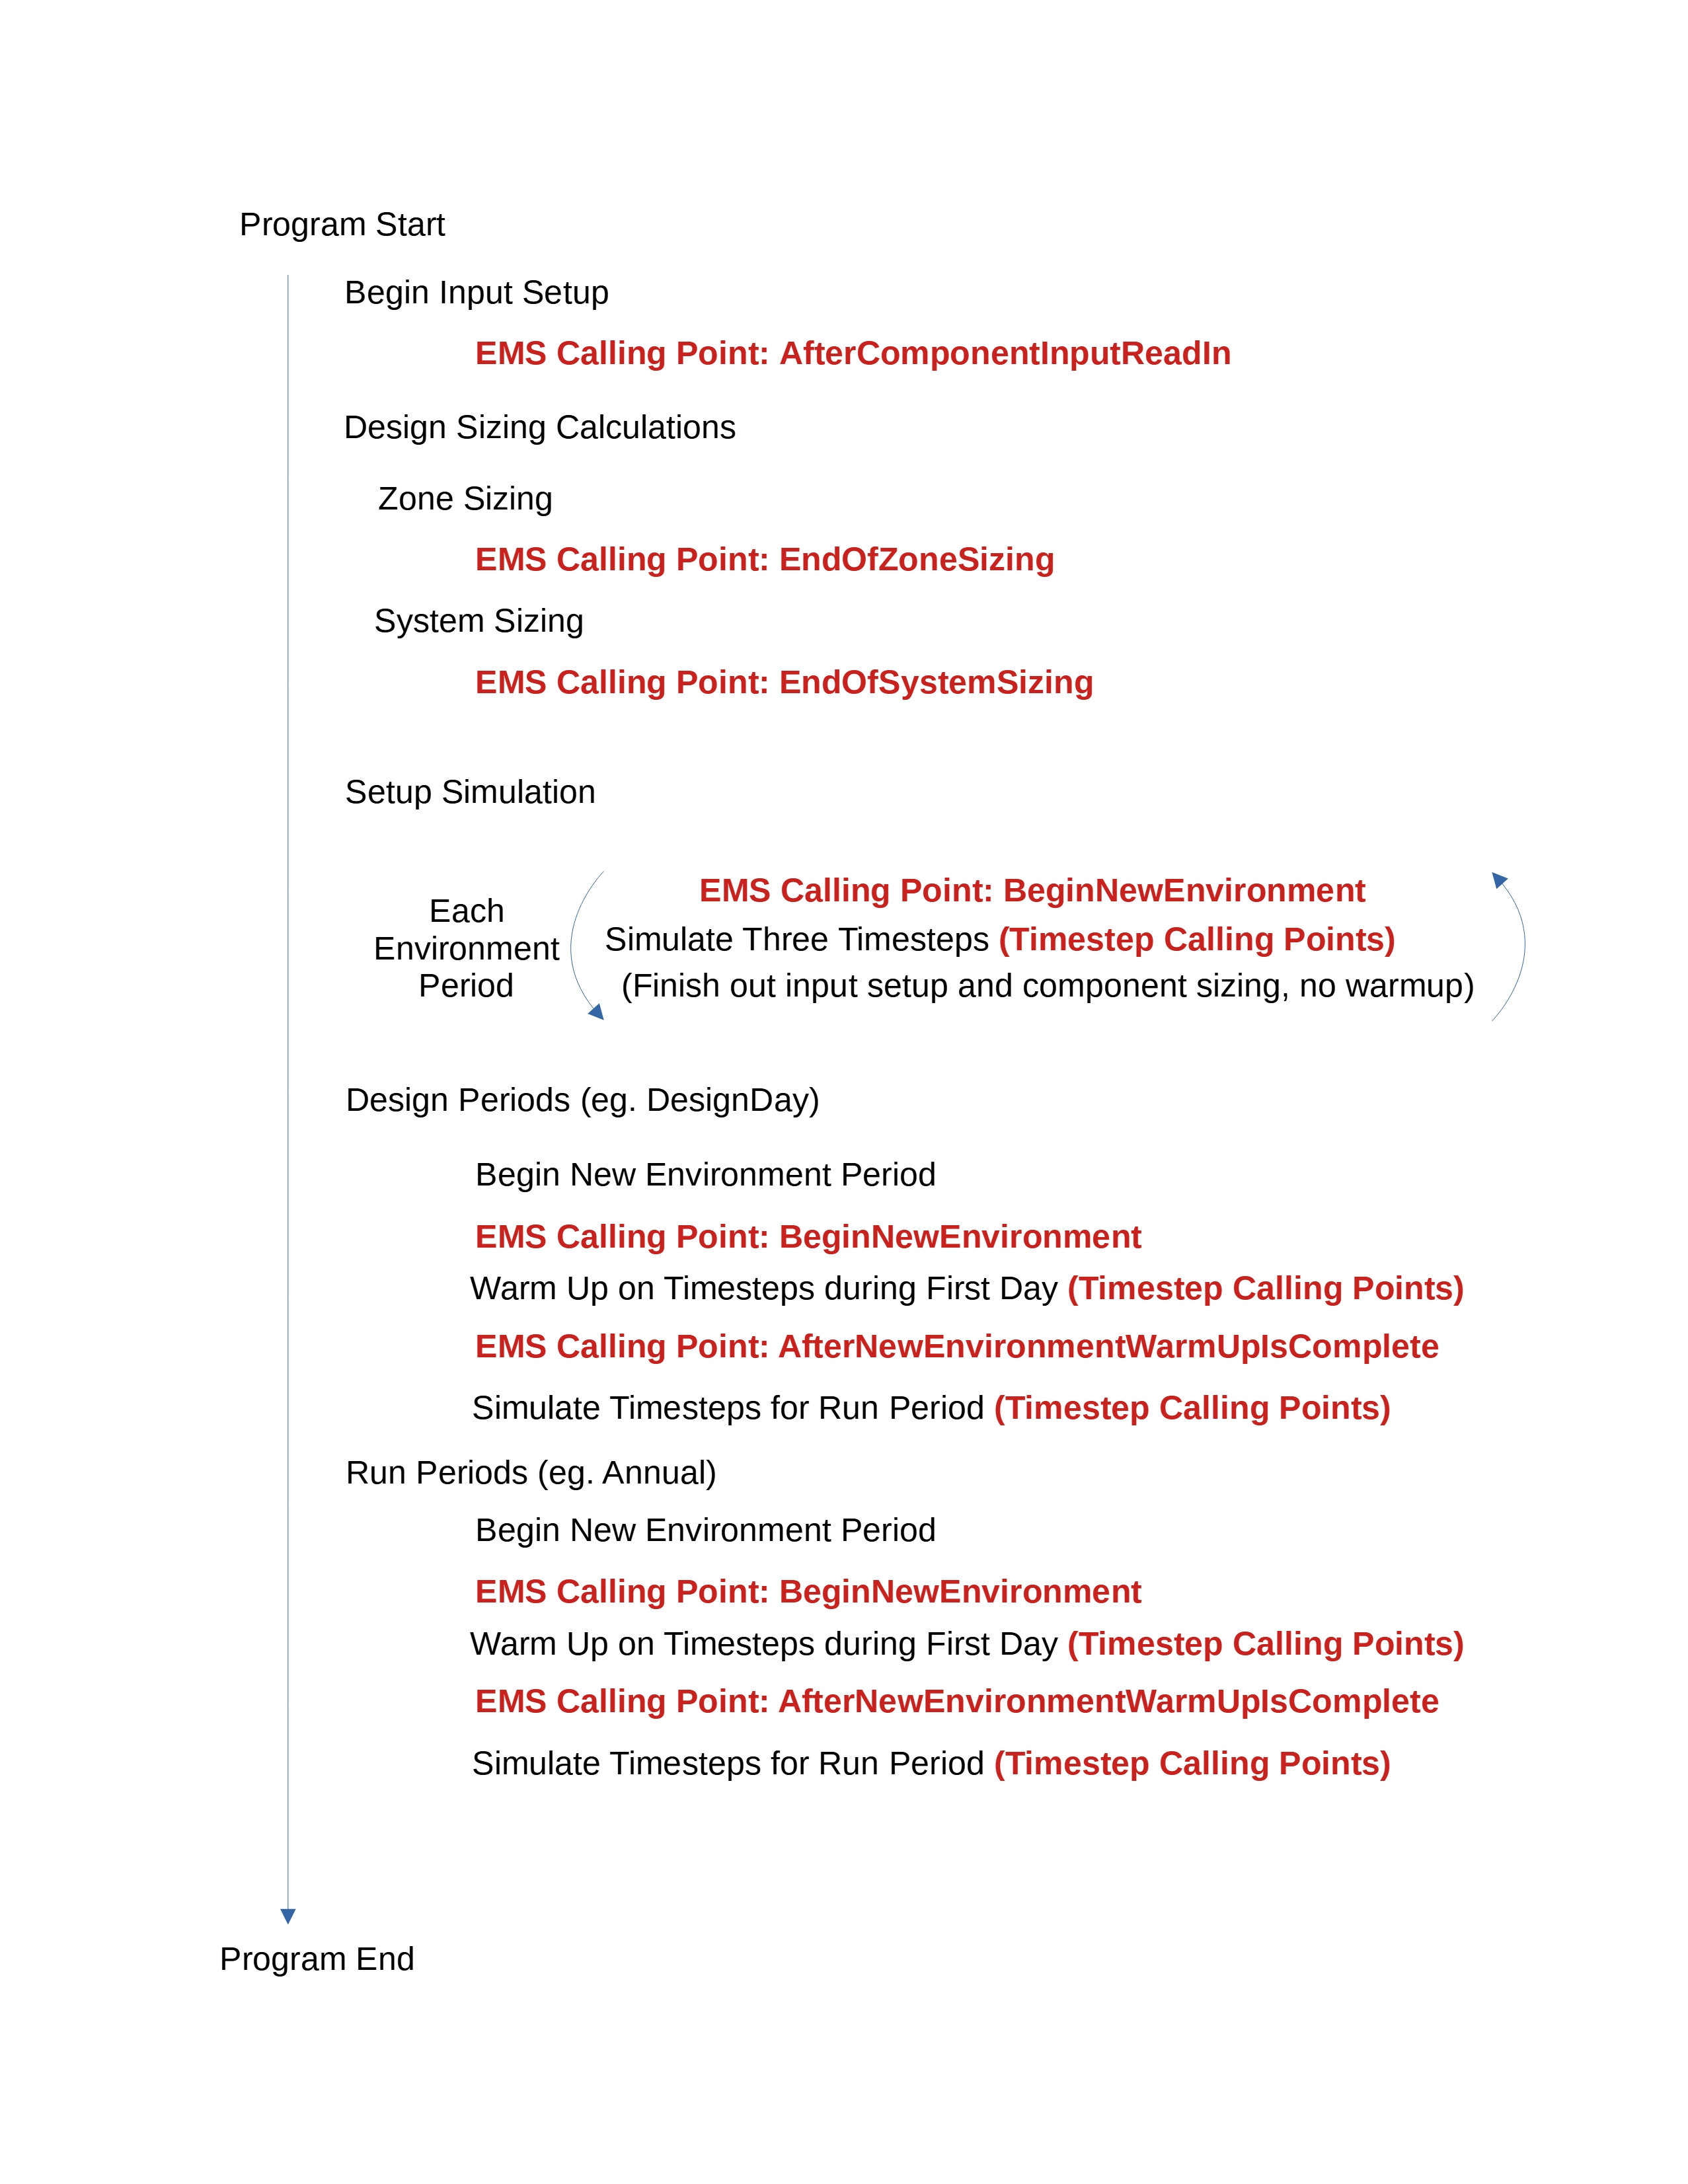
\includegraphics[width=0.9\textwidth, height=0.9\textheight, keepaspectratio=true]{media/image003.jpg}
\caption{Overall Program Flow and EMS Calling Points \protect \label{fig:overall-program-flow-and-ems-calling-points}}
\end{figure}

\begin{figure}[hbtp] % fig 2
\centering
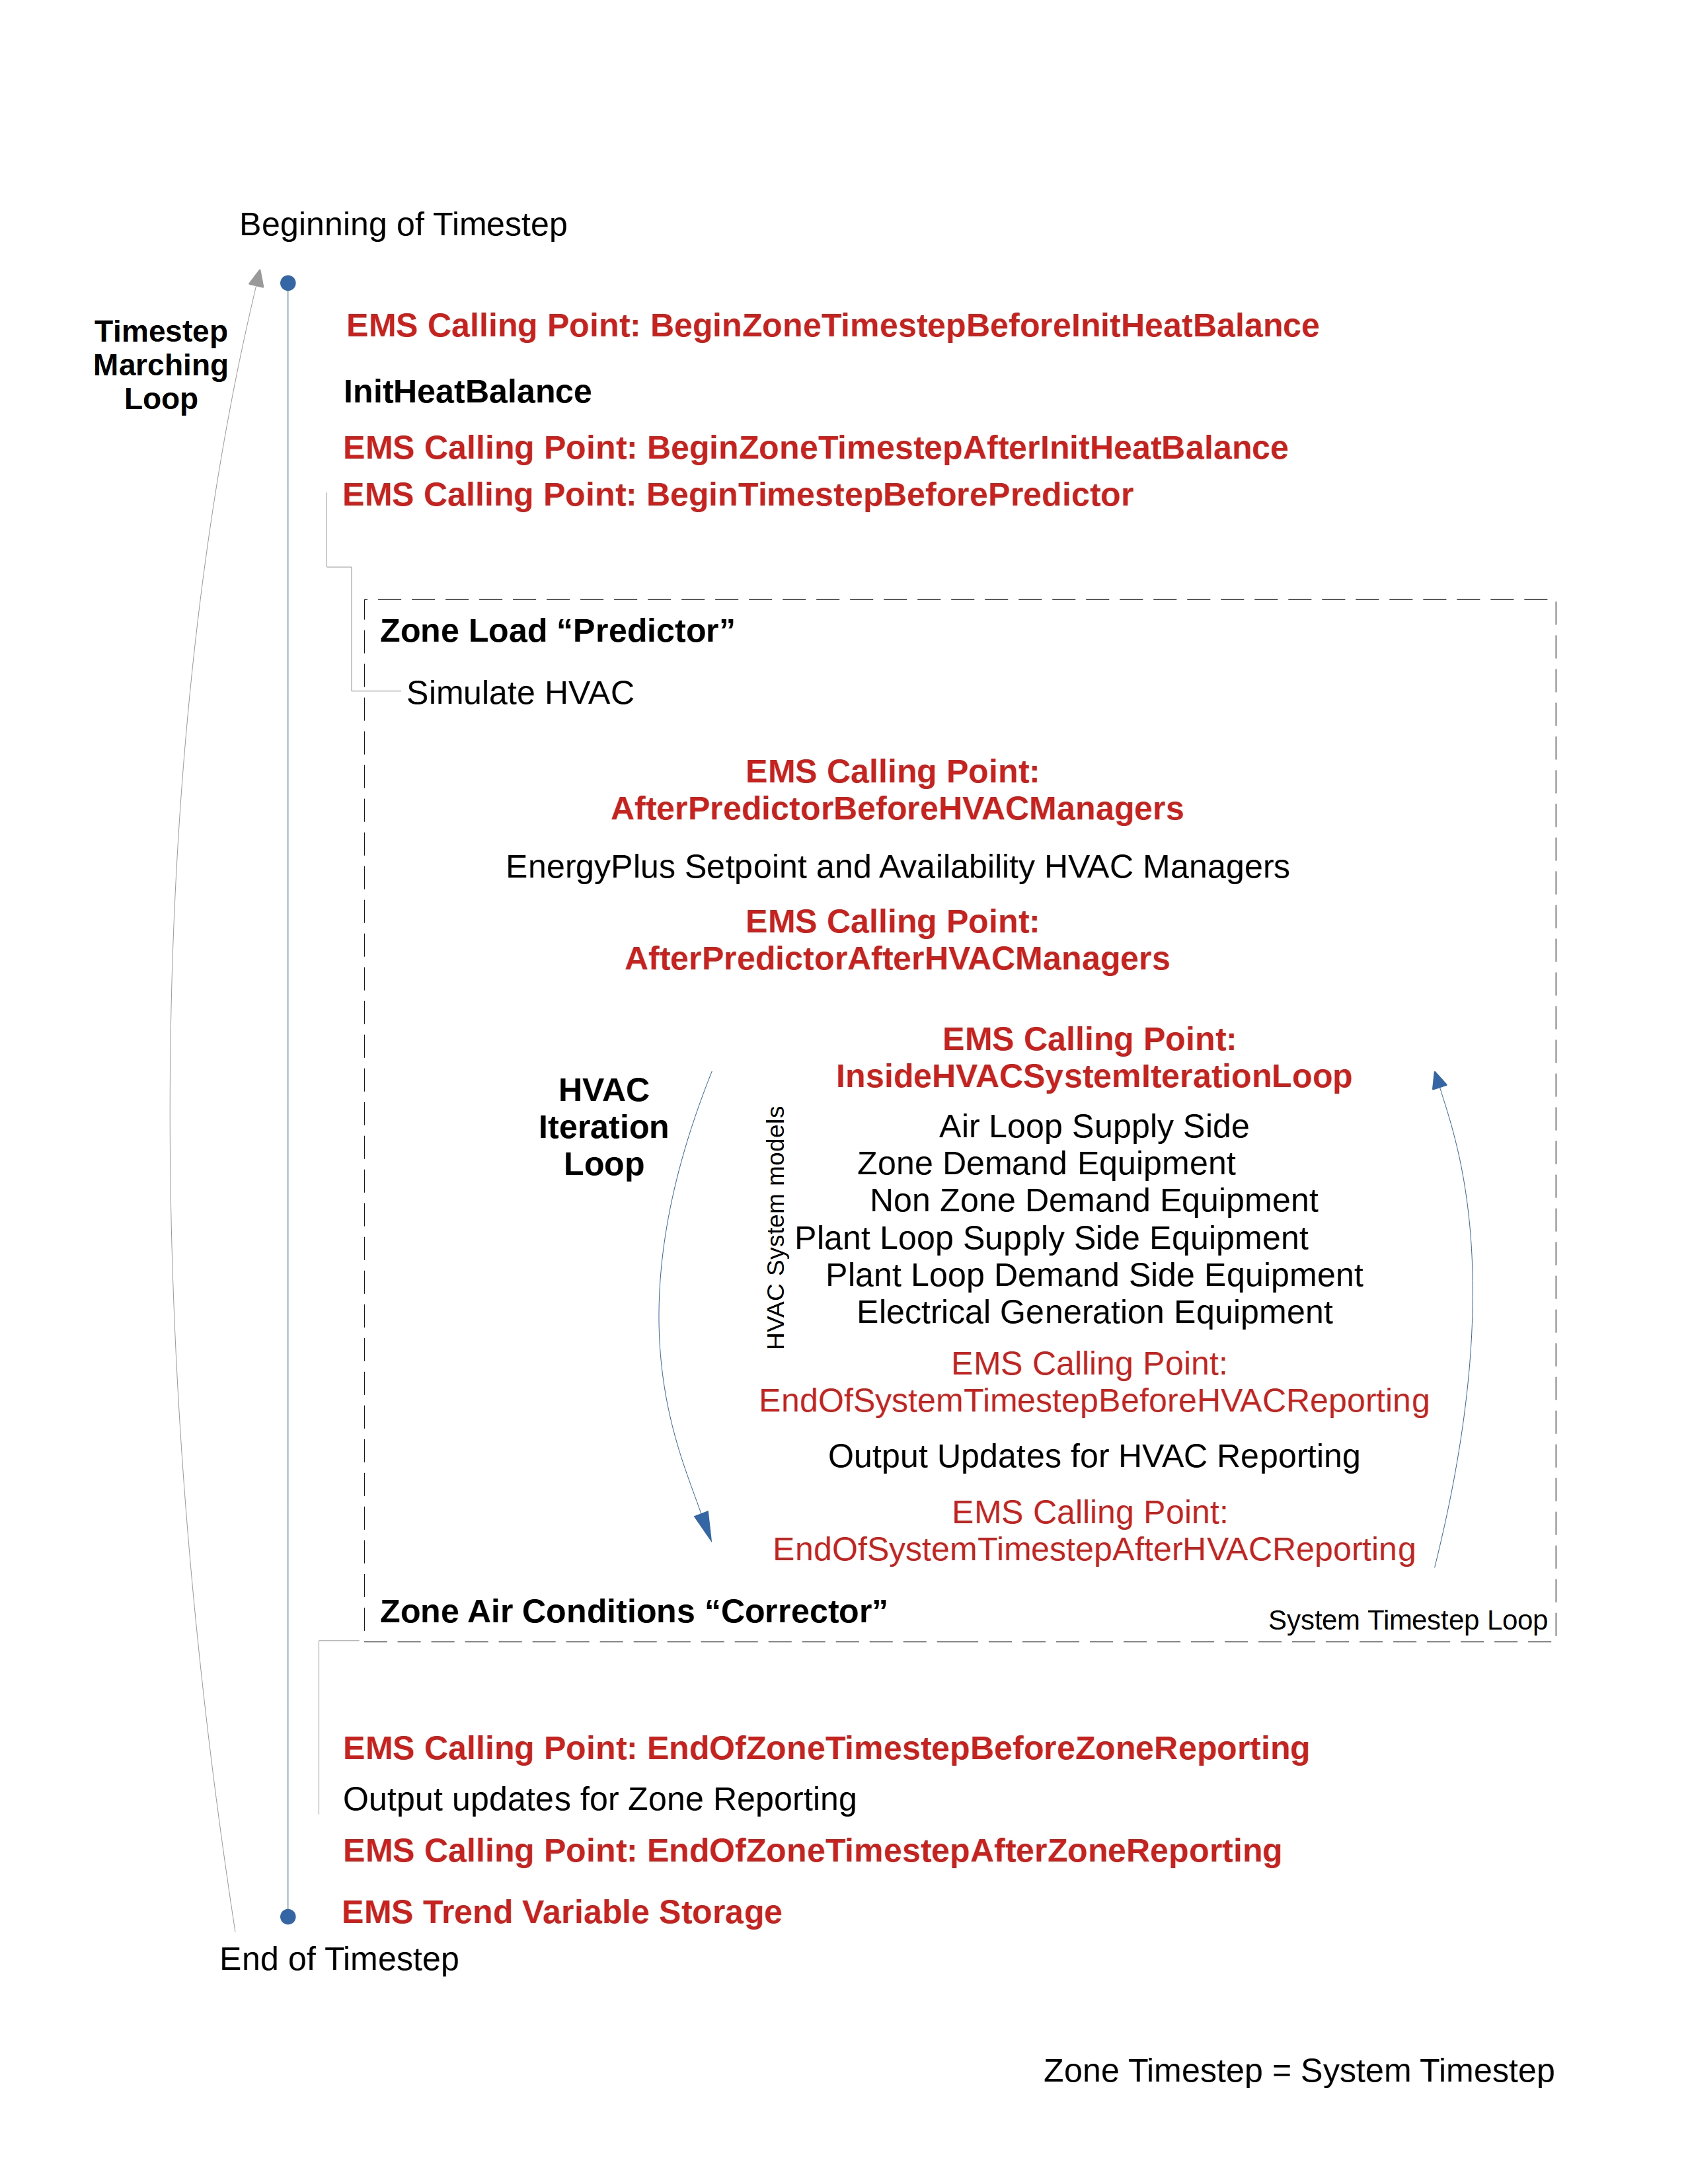
\includegraphics[width=0.9\textwidth, height=0.9\textheight, keepaspectratio=true]{media/image004.jpg}
\caption{Timestep Sequence with EMS Calling Points \protect \label{fig:timestep-sequence-with-ems-calling-points}}
\end{figure}

\begin{figure}[hbtp] % fig 3
\centering
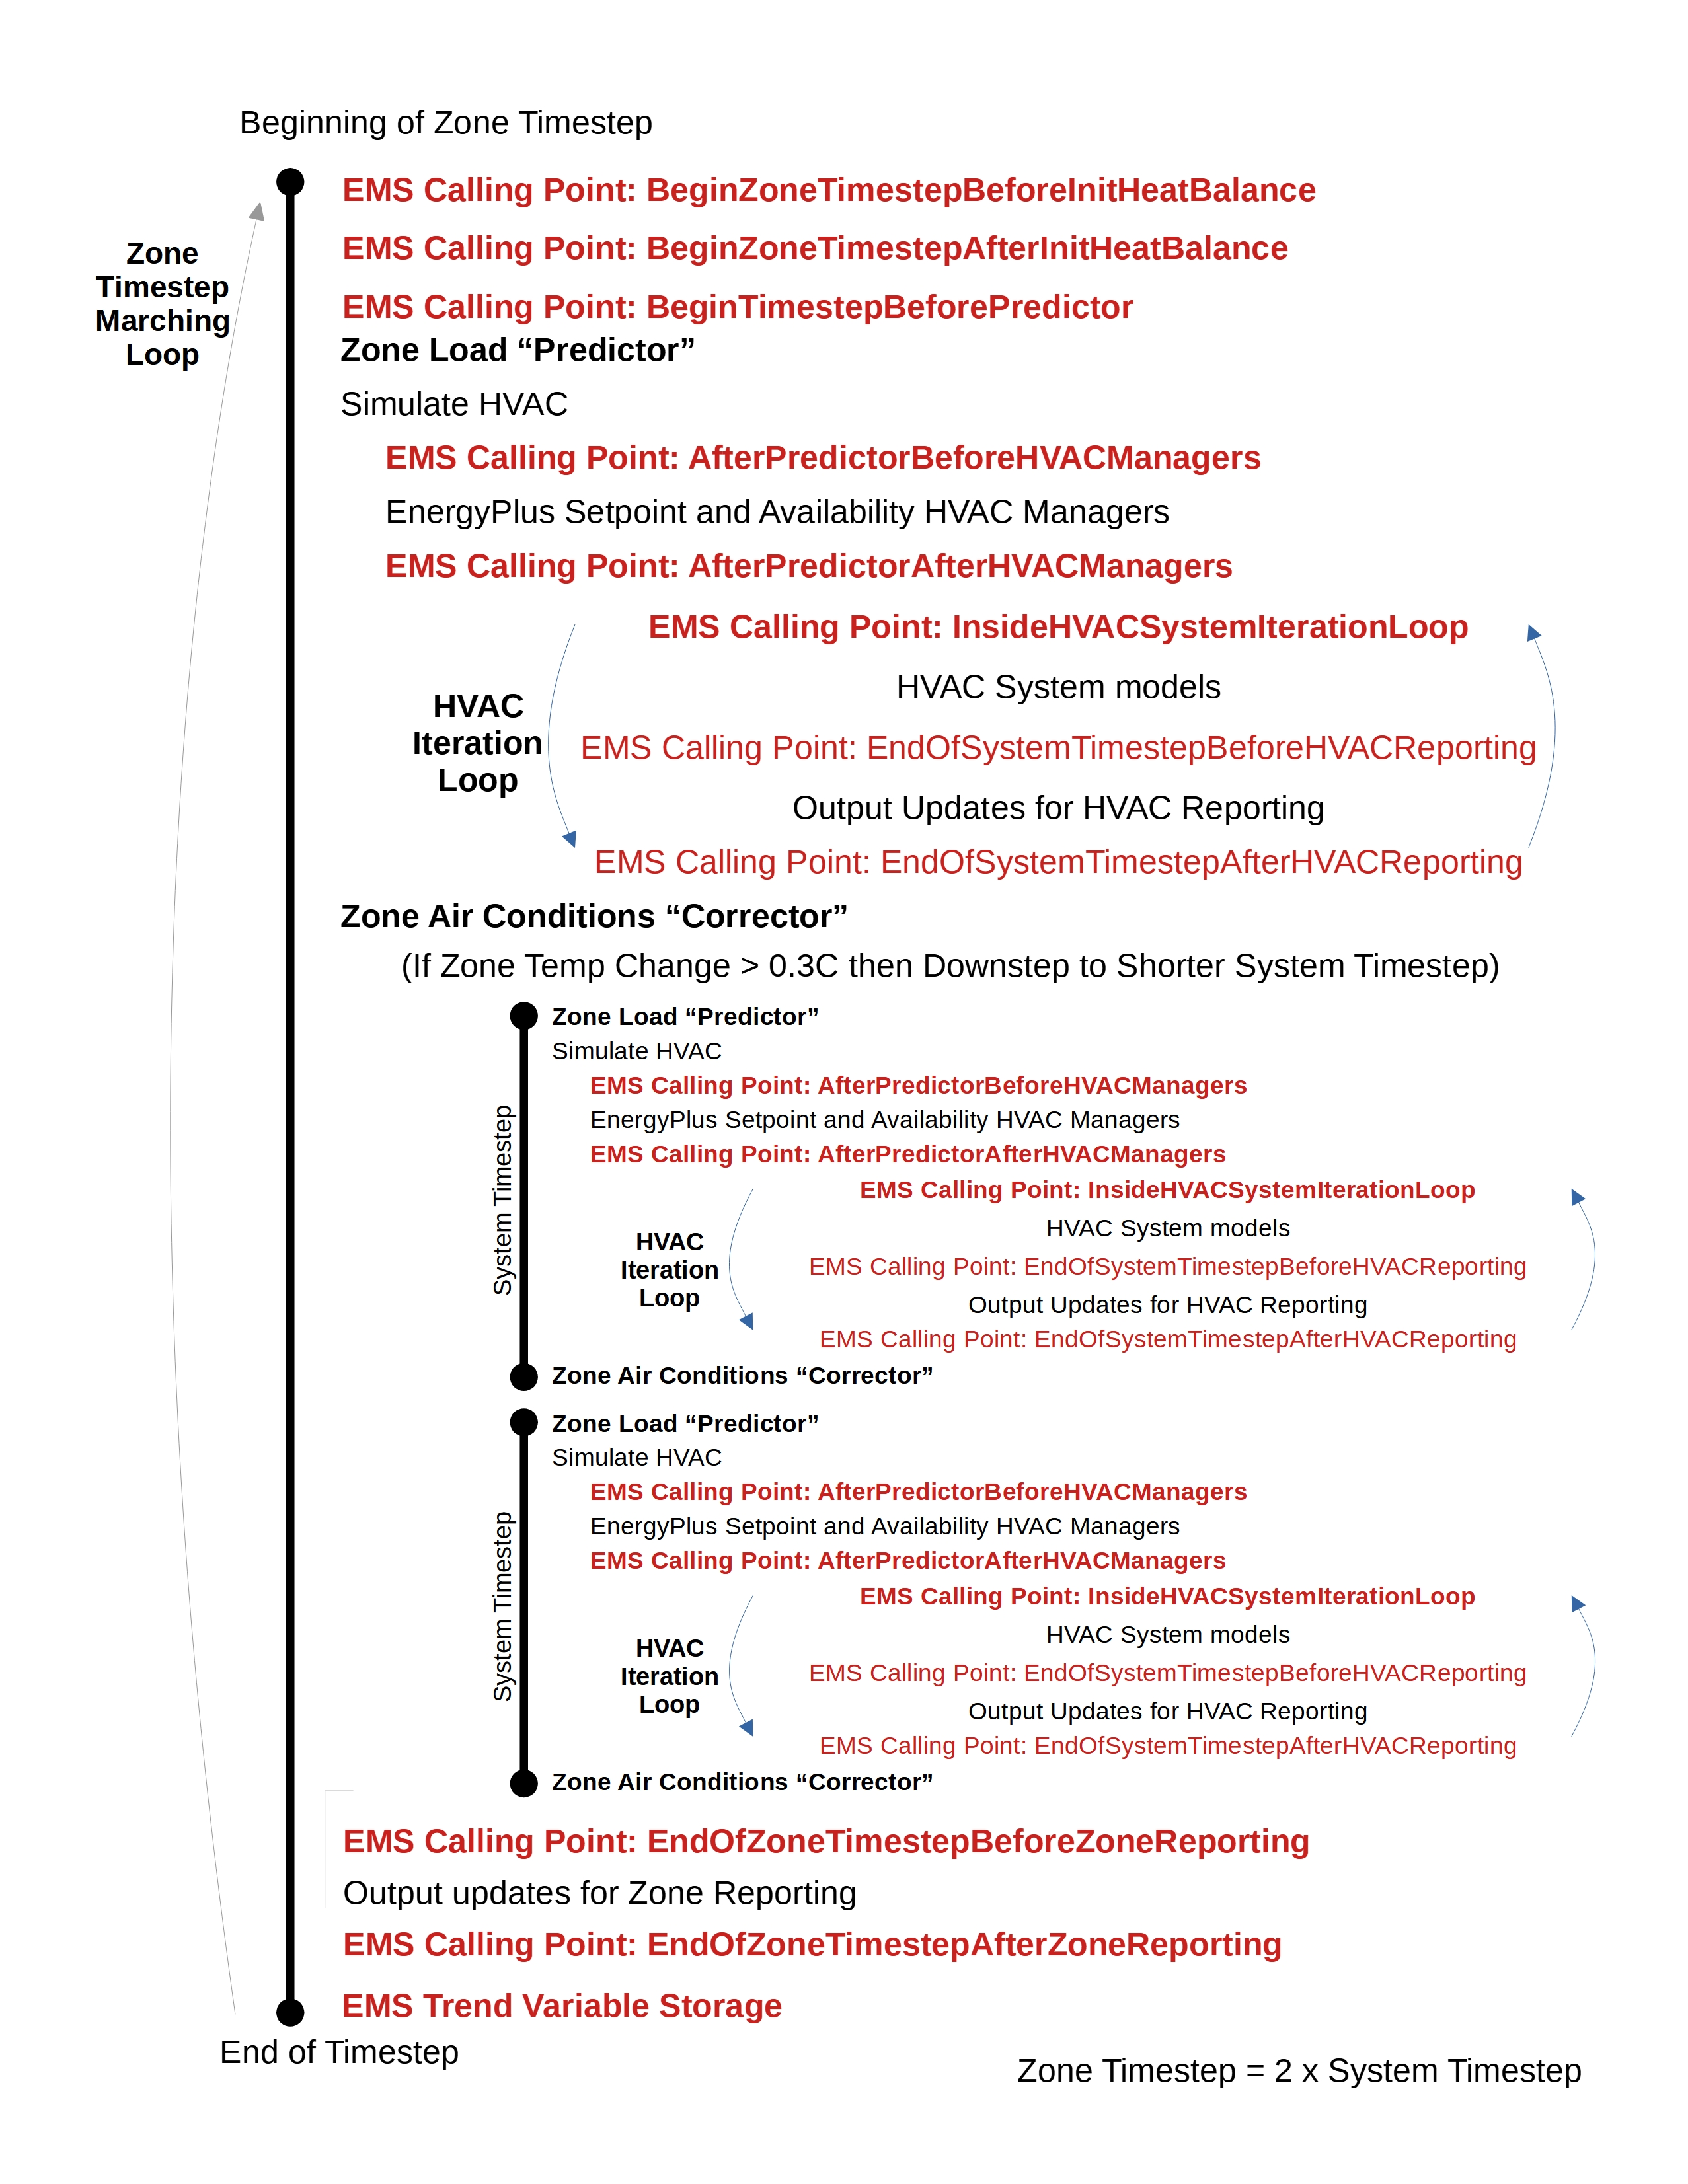
\includegraphics[width=0.9\textwidth, height=0.9\textheight, keepaspectratio=true]{media/image005.jpg}
\caption{System Timestep Sequence with EMS Calling Points \protect \label{fig:system-timestep-sequence-with-ems-calling}}
\end{figure}

When EnergyPlus runs a model, it first does various sizing and setup activities and then models the environment periods you ask for; e.g., design days and run periods. The built-in variable called CurrentEnvironment indentifies which of these is being simulated and any given time. Figure~\ref{fig:overall-program-flow-and-ems-calling-points} diagrams the overall program flow starting at the top and listing certain key steps in outline form. EnergyPlus models contain a lot of input, and the internal processes to acquire and process that input take some time to complete. Before the model starts doing final calculations, it may have to do various sizing calculations and automatically design the size of components. It will also go through special setup periods that model a truncated set of timesteps for each environment period. In the diagram, this initial phase is not finished until just before the design periods begin. Two EMS calling points that occur only once in a given run, EndOfZoneSizing and EndOfSystemSizing, can be triggered during this initial setup phase. During the phase called ``Setup Simulation,'' the various timestep-based calling points diagrammed in Figure~\ref{fig:timestep-sequence-with-ems-calling-points} will also be called.

Another thing that happens during the setup phase described above is that individual HVAC component models access their input data and do various setup calculations in preparation for the rest of the simulation.~~ An EMS calling point (added for Version 7) called ``AfterComponentInputReadIn'' is available for selected HVAC components that allows triggering Erl programs at a point just after the component's input data have been read in but before the component's sizing routines have executed.~ This calling point is intended to be used with various actuators that are setup to override the autosize values that result from sizing.

To model environment periods, EnergyPlus runs through a serious of timesteps. Figure~\ref{fig:timestep-sequence-with-ems-calling-points} diagrams the program flow for a single timestep where the timestep for the system modeling is equal to that for the zone load modeling. The \emph{system} timestep can be shorter than the \emph{zone} timestep. The usual process of modeling a timestep is to first calculate the zone loads during the ``Predictor,'' then model the response of the HVAC systems, and then calculate the resulting zone conditions during the ``Corrector.''~ Within the HVAC system modeling, some system iterations are used to iteratively solve a system of systems. Figure~\ref{fig:system-timestep-sequence-with-ems-calling} is a slightly modified version Figure~\ref{fig:timestep-sequence-with-ems-calling-points} that diagrams the situation when the timestep of the system calculations has been reduced to half the length of the zone timestep.


\section{Begin New Environment}\label{begin-new-environment}

The calling point referred to with the keyword ``BeginNewEnvironment'' occurs once near the beginning of each environment period. Environment periods include sizing periods, design days, and run periods. This calling point will not be useful for control actions, but is useful for initializing variables and calculations that do not need to be repeated during each timestep. Once a value is set, Erl variables remember the value during the remainder of the environment period. However, they are automatically reinitialized to 0.0 at the beginning of each new environment period and this calling point executed again to redo the initializations. Considerable repetition can be avoided by designing Erl programs to use this calling point for initializations and calculations that are needed only once for each environment period. It is not called during individual timesteps. It is not called until well into the simulation after sizing and the final setup of actuators and internal variables. 


\section{After New Environment Warmup Is Complete}\label{after-new-environment-warmup-is-complete}

The calling point referred to with the keyword ``AfterNewEnvironmentWarmUpIsComplete'' occurs once near at the beginning of each environment period but after any warmup days are complete. This is similar to the previous calling point. Warmup days are used to condition the transient aspects of the model before proceeding with the first day. This will not be useful for control actions, but would be useful for reinitializing Erl programs with fresh values after the warmup days have finished running and the model is about to start the final timestep calculations for a particular environment period.


\section{Begin Zone Timestep Before Init Heat Balance}\label{begin-timestep-before-init-heat-balance}

The calling point called ``BeginZoneTimestepBeforeInitHeatBalance'' occurs at the beginning of each timestep before ``InitHeatBalance'' executes but after the weather manager and exterior energy use manager. ``InitHeatBalance'' refers to the step in EnergyPlus modeling when the solar shading and daylighting coefficients are calculated. This calling point is useful for controlling components that affect the building envelope including surface constructions, window shades, and shading surfaces. Programs called from this point might actuate the building envelope or internal gains based on current weather or on the results from the previous timestep. Demand management routines might use this calling point to operate window shades, change active window constructions, activate exterior shades, etc.

\section{Begin Zone Timestep After Init Heat Balance}\label{begin-timestep-after-init-heat-balance}

The calling point called ``BeginZoneTimestepAfterInitHeatBalance'' occurs at the beginning of each timestep after ``InitHeatBalance'' executes and before ``ManageSurfaceHeatBalance''. ``InitHeatBalance'' refers to the step in EnergyPlus modeling when the solar shading and daylighting coefficients are calculated. This calling point is useful for controlling components that affect the building envelope including surface constructions and window shades. Programs called from this point might actuate the building envelope or internal gains based on current weather or on the results from the previous timestep. Demand management routines might use this calling point to operate window shades, change active window constructions, etc. This calling point would be an appropriate place to modify weather data values.

\section{Begin Timestep Before Predictor}\label{begin-timestep-before-predictor}

The calling point called ``BeginTimestepBeforePredictor'' occurs near the beginning of each timestep but before the predictor executes. ``Predictor'' refers to the step in EnergyPlus modeling when the zone loads are calculated. This calling point is useful for controlling components that affect the thermal loads the HVAC systems will then attempt to meet. Programs called from this point might actuate internal gains based on current weather or on the results from the previous timestep. Demand management routines might use this calling point to reduce lighting or process loads, change thermostat settings, etc.


\section{After Predictor Before HVAC Managers}\label{after-predictor-before-hvac-managers}

The calling point called ``AfterPredictorBeforeHVACManagers'' occurs after predictor and before the traditional HVAC managers are called. It occurs at each timestep just after the predictor executes but before SetpointManager and AvailabilityManager models are called. It is useful for a variety of control actions. However, if there are conflicts, the EMS control actions could be overwritten by other SetpointManager or AvailabilityManager actions.


\section{After Predictor After HVAC Managers}\label{after-predictor-after-hvac-managers}

The calling point called ``AfterPredictorAfterHVACManagers'' occurs after the predictor and after the traditional HVAC managers have been called. It occurs at each timestep after the predictor executes and after the SetpointManager and AvailabilityManager models are called. It is useful for a variety of control actions. However, if there are conflicts, SetpointManager or AvailabilityManager actions may be overwritten by EMS control actions.


\section{Inside HVAC System Iteration Loop}\label{inside-hvac-system-iteration-loop}

The calling point called ``InsideHVACSystemIterationLoop'' occurs before HVAC systems are modeled. Within a timestep, EnergyPlus loops over the HVAC model to solve a system of systems. It recurs after each HVAC system iteration within each timestep and can be used for a variety of control actions that affect system operation. Being within the iteration loop can increase the accuracy of control modeling when the inputs to the controls are also changing interactively. The disadvantage is extra computational expense.


\section{End of Zone Timestep Before Reporting}\label{end-of-zone-timestep-before-reporting}

The calling point called ``EndOfZoneTimestepBeforeZoneReporting'' occurs near the end of a zone timestep but before output variable reporting is finalized. It is useful for custom output variables that use the ZoneTimestep reporting frequency.


\section{End of Zone Timestep After Reporting}\label{end-of-zone-timestep-after-reporting}

The calling point called ``EndOfZoneTimestepAfterZoneReporting'' occurs at the end of a zone timestep after output variable reporting is finalized. It is useful for preparing calculations that will go into effect the next timestep. Its capabilities are similar to BeginTimestepBeforePredictor, except that input data for current time, date, and weather data align with different timesteps.


\section{End of System Timestep Before HVAC Reporting}\label{end-of-system-timestep-before-hvac-reporting}

The calling point called ``EndOfSystemTimestepBeforeHVACReporting'' occurs near the end of a system timestep but before output variable reporting is finalized. It is useful for custom output variables that use the SystemTimestep reporting frequency.


\section{End of System Timestep After HVAC Reporting}\label{end-of-system-timestep-after-hvac-reporting}

The calling point called ``EndOfSystemTimestepAfterHVACReporting'' occurs at the end of a system timestep after output variable reporting is finalized.


\section{End of Zone Sizing}\label{end-of-zone-sizing}

The calling point called ``EndOfZoneSizing'' is used to alter the results of zone sizing calculations. It executes only once per simulation during the early stages and only if the model includes zone sizing calculations. It is not useful for control applications.


\section{End of System Sizing}\label{end-of-system-sizing}

The calling point called ``EndOfSystemSizing'' is used to alter the results of air system sizing calculations. It executes only once per simulation and is not useful for control applications.


\section{After Component Model Input has Been Read In}\label{after-component-model-input-has-been-read-in}

The calling point called ``AfterComponentInputReadIn'' is used to alter the results of individual autosize fields.~ It executes whenever one of the selected components has finished reading in its input data.~ Those, and only those, component models that have some type of actuator with an ``Autosized'' control type will also have this calling point.~ This same calling point identifier is used for different HVAC components so programs executed from this point will be repeated.~ Currently this calling point exists in three different places:~ (1) after DX coil input, (2) after fan input, and (3) after unitary system input.


\section{User Defined Component Model}\label{user-defined-component-model}

The calling point called ``UserDefinedComponentModel'' is used with Erl programs that are associated with user defined component models.~ This calling point is executed whenever a user-defined component model is called to simulate.~ The user defined component models track which program calling managers are associated with the specific component and only those calling managers are executed when this calling point is triggered. This calling point is only used with calling managers referenced by the following input objects: PlantComponent:UserDefined, Coil:UserDefined, ZoneHVAC:ForcedAir:UserDefined, or AirTerminal:SingleDuct:UserDefined.


\chapter{User-Defined Component Models}\label{user-defined-component-models}

This section provides an overview of how you can use EMS to create your own custom models for HVAC and plant equipment.~ EMS can be used not only for controls and overriding the behavior of existing models, but also to implement entirely new component models of your own formulation.~ Such user-defined component models are implemented by writing Erl programs, setting up internal variables, sensors, actuators and output variables that work in conjunction with a set of special input objects in the group called ``User Defined HVAC and Plant Component Models.''

This system provides a means of modeling new types of equipment that do not yet have models implemented in EnergyPlus.~ The capability to add new custom models should have a wide variety of creative applications such as evaluating the annual energy performance implications of new types of equipment and providing a mechanism for including ``exceptional calculation methods'' in your EnergyPlus models.

This section first introduces common characteristics of the user-defined component models and then goes into more detail on each of available component modeling shells that are used to connect user-defined models and algorithms to the rest of EnergyPlus' HVAC and plant simulations.


\section{Common Characteristics}\label{common-characteristics}

In general, each of the user-defined components will:

\begin{itemize}
\item
  Setup new EMS internal variables for the state conditions entering the component at each inlet node being used.~ Internal variables serve a similar role as Sensors in terms of obtaining input data.~ The difference is that they are updated just before the component model programs execute and therefore do not suffer the timestep lag issues that can be associated with sensors tied to output variables.~ Whereas most EMS internal variables are constants, those intended for use with user-defined components are filled each time the component is simulated and vary over time with the most current data available.
\item
  Setup new EMS actuators for the state conditions at each outlet node being used.~ These actuators are not optional and must be used.~ For each air or plant connection with an active outlet node, the associated actuators must be used and filled with valid values in order for the component model to be properly coupled to the rest of EnergyPlus.~ Some of the components will also set the results at their inlet node, for example to request a mass flow rate.
\item
  Trigger one or more specific program calling manager(s) to execute EMS programs that are called to initialize, register, and size the component model.
\item
  Trigger one or more specific program calling manager(s) to execute EMS programs that are called to actually model the component when it is called to be simulated.
\end{itemize}

The various user-defined components have some similar input fields.~ Once the user gains familiarity with one of the components, many of the concepts will carry over to the other user-defined components.~ The separate objects are primarily for the purpose of distinguishing how user-defined components need to vary in order to fit with the rest of EnergyPlus.


\section{Zone Forced Air Unit}\label{zone-forced-air-unit}

The input object called ZoneHVAC:ForcedAir:UserDefined provides a shell for creating custom models of a device that serves as a single-zone HVAC unit that operates by circulating air in and out of the zone.~ This device is analogous to those component models in the Group -- Zone Forced Air Units, such as ZoneHVAC:PackagedTerminalAirConditioner or ZoneHVAC:WaterToAirHeatPump.

In addition to the primary air connection that connects to the zone, there are options for additional connections to a second air stream (e.g.~for outdoor ventilation or heat source or sink), up to three separate plant loop connections (e.g.~hot water, chilled water, heat rejection), a water supply tank, a water collection tank, and a separate zone for skin losses.

The zone unit is associated with a thermal zone (by the ZoneHVAC:EquipmentConnections and ZoneHVAC:EquipmentList objects).~ In EnergyPlus, when there are controlled thermal zones with thermostat (and humidistat) controls, the central routines predict the loads that zone equipment need to meet in order to maintain control of the zone conditions.~ When there are multiple types of equipment serving a zone, they are sequenced to meet heating or cooling loads in a particular order.~ Rather than the total predicted load, the second or third devices need to know the load that remains after the earlier-sequenced devices have already operated on the zone.~ The following internal variables are useful inputs for controlling zone equipment in your models:

\begin{itemize}
\item
  An internal variable called ``Remaining Sensible Load to Heating Setpoint'' provides the current value for the sensible load, in {[}W{]}, that remains for this device that if delivered will allow the zone to reach the heating setpoint under current conditions.
\item
  An internal variable called ``Remaining Sensible Load to Cooling Setpoint'' provides the current value for the sensible load, in {[}W{]}, that remains for this device that if delivered will allow the zone to reach the cooling setpoint under current conditions.
\item
  An internal variable called ``Remaining Latent Load to Humidifying Setpoint'' provides the current value for the latent load, in {[}kg/s{]}, that remains for this device that if delivered will allow the zone to reach the humidification setpoint under current conditions.
\item
  An internal variable called ``Remaining Latent Load to Dehumidifying Setpoint'' provides the current value for the latent load, in {[}kg/s{]}, that remains for this device that if delivered will allow the zone to reach the dehumidification setpoint under current conditions.
\end{itemize}

\subsection{Primary Air Connection}\label{primary-air-connection-000}

The primary air connection includes both an inlet and an outlet that are required to be used when using this component.~ This is called the primary air connection because it is how the zone unit is connected to the zone.~ The inlet to the custom zone unit is a node that is also an exhaust outlet from the zone.~ The following EMS internal variables are made available for this inlet node and should be useful inputs to your own custom models:

\begin{itemize}
\item
  An internal variable called ``Inlet Temperature for Primary Air Connection,'' provides the current value for the drybulb air temperature at the component's inlet node, in {[}C{]}.
\item
  An internal variable called ``Inlet Humidity Ratio for Primary Air Connection,'' provides the current value for the moist air humidity ratio at the component's inlet node, in {[}kgWater/kgDryAir{]}
\item
  An internal variable called ``Inlet Density for Primary Air Connection,'' provides the current value for the density of moist air at the component's main inlet node, in {[}kg/m\(^{3}\){]}.
\item
  An internal variable called ``Inlet Specific Heat for Primary Air Connection,'' provides the current value for the specific heat of moist air at the component's main inlet node, in {[}J/kg-C{]}.
\end{itemize}

The inlet node also has an actuator associated with it so that the rate of air flow leaving the thermal zone and entering the unit can be passed to the rest of EnergyPlus.

\begin{itemize}
\tightlist
\item
  An actuator called ``Primary Air Connection,'' with the control type ``Inlet Mass Flow Rate,'' in {[}kg/s{]}, needs to be used.~ This will set the flow rate of air leaving the zone through the zone exhaust air node.
\end{itemize}

The primary outlet for the custom zone unit is a node that is also an inlet to the zone.~ The following EMS actuators are created for this outlet node and must be used to pass results from the custom model to the rest of EnergyPlus:

\begin{itemize}
\item
  An actuator called ``Primary Air Connection,'' with the control type ``Outlet Temperature,'' in {[}C{]}, needs to be used.~ This will set the drybulb temperature of the air leaving the zone unit and entering the zone through the zone air inlet node.
\item
  An actuator called ``Primary Air Connection,'' with the control type ``Outlet Humidity Ratio,'' in {[}kgWater/kgDryAir{]}, needs to be used.~ This will set the humidity ratio of the air leaving the zone unit and entering the zone through the zone air inlet node.
\item
  An actuator called ``Primary Air Connection,'' with the control type ``Outlet Mass Flow Rate,'' in {[}kg/s{]}, needs to be used.~ This will set the flow rate of air leaving the zone unit and entering the zone through the zone air inlet node.
\end{itemize}

It is not required that the primary air connections inlet and outlet mass flow rates be identical.~ However, if there is an imbalance, then the model should use the secondary air connection to balance air mass flows.

\subsection{Secondary Air Connection}\label{secondary-air-connection-000}

The secondary air connection provides options for an added inlet node, or outlet node, or both depending on the user's needs.~ This separate air stream can be used for outdoor air ventilation or as a source or sink for energy.~ The secondary air inlet node will often be defined to be an outdoor air node (ref. OutdoorAir:Node) but that is not required.~ The secondary air outlet node can be used as relief exhaust when the unit is providing outdoor air ventilation.~ If the secondary air outlet is not really connected to anything else and just releases air to the outdoors, then it isn't necessary that moist air properties be set using actuators because they will not impact anything else in the model.

If the secondary air connection inlet node is used, then the following internal variables and actuator are made available:

\begin{itemize}
\item
  An internal variable called ``Inlet Temperature for Secondary Air Connection,'' provides the current value for the drybulb air temperature at the secondary inlet node, in {[}C{]}.
\item
  An internal variable called ``Inlet Humidity Ratio for Secondary Air Connection,'' provides the current value for the moist air humidity ratio at the secondary inlet node, in {[}kgWater/kgDryAir{]}
\item
  An internal variable called ``Inlet Density for Secondary Air Connection,'' provides the current value for the density of moist air at the secondary inlet node, in {[}kg/m\(^{3}\){]}.
\item
  An internal variable called ``Inlet Specific Heat for Secondary Air Connection,'' provides the current value for the specific heat of moist air at the secondary inlet node, in {[}J/kg-C{]}.
\item
  An actuator called ``Secondary Air Connection,'' with the control type ``Inlet Mass Flow Rate,'' in {[}kg/s{]}, needs to be used.~ This will set the flow rate of air entering the zone unit through the secondary air connection inlet.
\end{itemize}

If the secondary air connection outlet node is used, then the following actuators are created:

\begin{itemize}
\item
  An actuator called ``Secondary Air Connection,'' with the control type ``Outlet Temperature,'' in {[}C{]}, needs to be used.~ This will set the drybulb temperature of the air leaving the zone unit through the secondary air outlet node.
\item
  An actuator called ``Secondary Air Connection,'' with the control type ``Outlet Humidity Ratio,'' in {[}kgWater/kgDryAir{]}, needs to be used.~ This will set the humidity ratio of the air leaving the zone unit through the secondary air outlet node.
\item
  An actuator called ``Secondary Air Connection,'' with the control type ``Outlet Mass Flow Rate,'' in {[}kg/s{]}, needs to be used.~ This will set the flow rate of air leaving the zone unit through the secondary air outlet node.
\end{itemize}

\subsection{Plant Connections}\label{plant-connections-002}

The user defined zone unit can also be connected to up to three different plants to provide hydronic-based cooling, heating, and/or heat source or rejection.

Although the zone unit actively conditions the zone, from the point of view of plant they are demand components.~ These plant connections are always ``demand'' in the sense that the zone unit will place loads onto the plant loops serving it and are not configured to be able to meet plant loads in the way that supply equipment could (loading mode is always DemandsLoad).~ These plant connections are always of the type that when flow is requested, the loop will be operated to try and meet the flow request and if not already running, these flow requests can turn on the loop (loop flow request mode is always NeedsFlowAndTurnsLoopOn).

For plant loops, both the inlet and outlet nodes need to be used for each loop connection.~ The ZoneHVAC:ForcedAir:UserDefined object appears directly on the Branch object used to describe the plant.~ The central plant routines require that each plant component be properly initialized and registered. Special actuators are provided for these initializations and they should be filled with values by the Erl programs that are called by the program calling manager assigned to the zone unit for model setup and sizing.~ The following three actuators are created for each of ``\emph{N}'' plant loops and must be used to properly register the plant connection:

\begin{itemize}
\item
  An actuator called ``Plant Connection \emph{N}'' with the control type ``Minimum Mass Flow Rate,'' in {[}kg/s{]}, should be used.~ This will set the so-called hardware limit for component's minimum mass flow rate when operating.~ (If not used, then the limit will be set to zero which may be okay for many if not most models.)
\item
  An actuator called ``Plant Connection \emph{N}'' with the control type ``Maximum Mass Flow Rate,'' in {[}kg/s{]}, needs to be used.~ This will set the so-called hardware limit for the component's maximum mass flow rate when operating.
\item
  An actuator called ``Plant Connection \emph{N}'' with the control type ``Design Volume Flow Rate,'' in {[}m\(^{3}\)/s{]}, needs to be used.~ This will register the size of the component for use in sizing the plant loop and supply equipment that will need to meet the loads.
\end{itemize}

For each plant loop connection that is used, the following internal variables are available for inputs to the custom component model:

\begin{itemize}
\item
  An internal variable called ``Inlet Temperature for Plant Connection \emph{N}'' provides the current value for the temperature of the fluid entering the component, in {[}C{]}.
\item
  An internal variable called ``Inlet Mass Flow Rate for Plant Connection \emph{N}'' provides the current value for the mass flow rate of the fluid entering the component, in {[}kg/s{]}.
\item
  An internal variable called ``Inlet Density for Plant Connection \emph{N}'' provides the current value for the density of the fluid entering the component, in {[}kg/m\(^{3}\){]}.~ This density is sensitive to the fluid type (e.g.~if using glycol in the plant loop) and fluid temperature at the inlet.
\item
  An internal variable called ``Inlet Specific Heat for Plant Connection \emph{N}'' provides the current value for the specific heat of the fluid entering the component, in {[}J/kg-C{]}. This specific heat is sensitive to the fluid type (e.g.~if using glycol in the plant loop) and fluid temperature at the inlet.
\end{itemize}

For each plant loop connection that is used, the following EMS actuators are created and must be used to pass results from the custom model to the rest of EnergyPlus:

\begin{itemize}
\item
  An actuator called ``Plant Connection \emph{N}'' with the control type ``Outlet Temperature,'' in {[}C{]}, needs to be used.~ This is the temperature of the fluid leaving the zone unit through that particular plant connection.
\item
  An actuator called ``Plant Connection N'' with the control type ``Mass Flow Rate,'' in kg/s, needs to be used. This actuator registers the component model's request for plant fluid flow.~ The actual mass flow rate through the component may be different than requested if the overall loop situation is such that not enough flow is available to meet all the various requests.~ In general, this actuator is used to lodge a request for flow, but the more accurate flow rate will be the internal variable called ``Inlet Mass Flow Rate for Plant Connection \emph{N.}''
\end{itemize}

\subsection{Water Use}\label{water-use-002}

The user defined zone unit can be connected to the water use models in EnergyPlus that allow modeling on-site storage.~ If a supply inlet water storage tank is used, then an actuator called ``Water System'' with the control type ``Supplied Volume Flow Rate,'' in m\(^{3}\)/s, needs to be used.~ This sets up the zone unit as a demand component for that storage tank.~ If a collection outlet water storage tank is used, then an actuator called ``Water System'' with the control type ``Collected Volume Flow Rate,'' in m\(^{3}\)/s, needs to be used.

\subsection{Ambient Zone}\label{ambient-zone-002}

The user defined zone unit can be connected to an ambient zone and provide internal gains to that zone.~ The zone can be different than the one that unit is connected to via the primary air connection if desired.~ This is for ``skin losses'' that the unit might have that result from inefficiencies and other non-ideal behavior.~ When an ambient zone is specified, the following actuators are created that can be used for different types of internal gains to the named zone:

\begin{itemize}
\item
  An actuator called ``Component Zone Internal Gain'' with the control type ``Sensible Heat Gain Rate,'' in {[}W{]}, is available.~ This can be used for purely convective sensible heat gains (or losses) to a zone.
\item
  An actuator called ``Component Zone Internal Gain'' with the control type ``Return Air Heat Gain Rate,'' in {[}W{]}, is available.~ This can be used for purely convective sensible heat gains (or losses) to the return air duct for a zone.
\item
  An actuator called ``Component Zone Internal Gain'' with the control type ``Thermal Radiation Heat Gain Rate,'' in {[}W{]}, is available.~ This can be used for thermal radiation gains (or losses) to a zone.
\item
  An actuator called ``Component Zone Internal Gain'' with the control type ``Latent Heat Gain Rate,' in {[}W{]}, is available.~ This can be used for latent moisture gains (or losses) to a zone.
\item
  An actuator called ``Component Zone Internal Gain'' with the control type ``Return Air Latent Heat Gain Rate,'' in {[}W{]}, is available.~ This can be used for latent moisture gains (or losses) to a the return air duct for a zone.
\item
  An actuator called ``Component Zone Internal Gain'' with the control type ``Carbon Dioxide Gain Rate,'' in {[}m\(^{3}\)/s{]}, is available.~ This can be used for carbon dioxide gains (or losses) to a zone.
\item
  An actuator called ``Component Zone Internal Gain'' with the control type ``Gaseous Contaminant Gain Rate,'' in {[}m\(^{3}\)/s{]}, is available.~ This can be used for generic gaseous air pollutant gains (or losses) to a zone.
\end{itemize}


\section{Air Terminal Unit}\label{air-terminal-unit}

The input object called AirTerminal:SingleDuct:UserDefined provides a shell for creating custom models for an air terminal that connects a multi-zone air handler to a thermal zone.~ This device is analogous to the single-duct terminal units in the Group -- Air Distribution Equipment, such as AirTerminal:SingleDuct:VAV:Reheat or AirTerminal:SingleDuct:ConstantVolume:FourPipeInduction.

In addition to the primary air connection that connects from the air loop to the zone, there are options for additional connections to a second air stream (e.g.~for outdoor ventilation or heat source or sink), up to two separate plant loop connections (e.g.~hot water and chilled water), a water supply tank, a water collection tank, and a separate zone for skin losses.

The air terminal unit is a associated with a thermal zone (by the ZoneHVAC:EquipmentConnections, ZoneHVAC:EquipmentList, and ZoneHVAC:AirDistributionUnit objects).~ In EnergyPlus, when there are controlled thermal zones with thermostat (and humidistat) controls, the central routines predict the loads that zone equipment need to meet in order to maintain control of the zone conditions.~ When there are multiple types of equipment serving a zone, they are sequenced to meet heating or cooling loads in a particular order.~ Rather than the total predicted load, the second or third devices need to know the load that remains after the earlier-sequenced devices have already operated on the zone.~ The following internal variables are useful inputs for controlling zone equipment in your models:

\begin{itemize}
\item
  An internal variable called ``Remaining Sensible Load to Heating Setpoint'' provides the current value for the sensible load, in {[}W{]}, that remains for this device that if delivered will allow the zone to reach the heating setpoint under current conditions.
\item
  An internal variable called ``Remaining Sensible Load to Cooling Setpoint'' provides the current value for the sensible load, in {[}W{]}, that remains for this device that if delivered will allow the zone to reach the cooling setpoint under current conditions.
\item
  An internal variable called ``Remaining Latent Load to Humidifying Setpoint'' provides the current value for the latent load, in {[}kg/s{]}, that remains for this device that if delivered will allow the zone to reach the humidification setpoint under current conditions.
\item
  An internal variable called ``Remaining Latent Load to Dehumidifying Setpoint'' provides the current value for the latent load, in {[}kg/s{]}, that remains for this device that if delivered will allow the zone to reach the dehumidification setpoint under current conditions.
\end{itemize}

\subsection{Primary Air Connection}\label{primary-air-connection}

The primary air connection includes both an inlet and an outlet that are required to be used when using this component.~ This called the primary air connection because it is how the terminal unit is connected from the air handle to the zone.~ The inlet to the custom air terminal unit is a node that is also the outlet from an AirLoopHVAC:ZoneSplitter object.~ The following EMS internal variables are made available for this inlet node and should be useful inputs to your own custom models:

\begin{itemize}
\item
  An internal variable called ``Inlet Temperature for Primary Air Connection,'' provides the current value for the drybulb air temperature at the component's inlet node, in {[}C{]}.
\item
  An internal variable called ``Inlet Humidity Ratio for Primary Air Connection,'' provides the current value for the moist air humidity ratio at the component's inlet node, in {[}kgWater/kgDryAir{]}
\item
  An internal variable called ``Inlet Density for Primary Air Connection,'' provides the current value for the density of moist air at the component's main inlet node, in {[}kg/m\(^{3}\){]}.
\item
  An internal variable called ``Inlet Specific Heat for Primary Air Connection,'' provides the current value for the specific heat of moist air at the component's main inlet node, in {[}J/kg-C{]}.
\end{itemize}

The inlet node also has an actuator associated with it so that the rate of air flow leaving the thermal zone and entering the unit can be passed to the rest of EnergyPlus.

\begin{itemize}
\tightlist
\item
  An actuator called ``Primary Air Connection,'' with the control type ``Inlet Mass Flow Rate,'' in {[}kg/s{]}, needs to be used.~ This will set the flow rate of air leaving the zone splitter and entering the air terminal unit.
\end{itemize}

The primary outlet for the custom air terminal unit is a node that is also an inlet to the zone.~ The following EMS actuators are created for this outlet node and must be used to pass results from the custom model to the rest of EnergyPlus:

\begin{itemize}
\item
  An actuator called ``Primary Air Connection,'' with the control type ``Outlet Temperature,'' in {[}C{]}, needs to be used.~ This will set the drybulb temperature of the air leaving the air terminal unit and entering the zone through the zone air inlet node.
\item
  An actuator called ``Primary Air Connection,'' with the control type ``Outlet Humidity Ratio,'' in {[}kgWater/kgDryAir{]}, needs to be used.~ This will set the humidity ratio of the air leaving the air terminal unit and entering the zone through the zone air inlet node.
\item
  An actuator called ``Primary Air Connection,'' with the control type ``Outlet Mass Flow Rate,'' in {[}kg/s{]}, needs to be used.~ This will set the flow rate of air leaving the air terminal unit and entering the zone through the zone air inlet node.
\end{itemize}

It is not required that the primary air connections inlet and outlet mass flow rates be identical.~ However, if there is an imbalance, then the model should use the secondary air connection to balance air mass flows.

\subsection{Secondary Air Connection}\label{secondary-air-connection}

The secondary air connection provides options for an added inlet node, or outlet node, or both depending on the user's needs.~ This separate air stream can be used for outdoor air ventilation or as a source or sink for energy.~ The secondary air inlet node will often be defined to be an outdoor air node (ref. OutdoorAir:Node) but that is not required.~ The secondary air outlet node can be used as relief exhaust when the unit is providing outdoor air ventilation.~ If the secondary air outlet is not really connected to anything else and just releases air to the outdoors, then it isn't necessary that moist air properties be set using actuators because they will not impact anything else in the model.

If the secondary air connection inlet node is used, then the following internal variables and actuator are made available:

\begin{itemize}
\item
  An internal variable called ``Inlet Temperature for Secondary Air Connection,'' provides the current value for the drybulb air temperature at the secondary inlet node, in {[}C{]}.
\item
  An internal variable called ``Inlet Humidity Ratio for Secondary Air Connection,'' provides the current value for the moist air humidity ratio at the secondary inlet node, in {[}kgWater/kgDryAir{]}
\item
  An internal variable called ``Inlet Density for Secondary Air Connection,'' provides the current value for the density of moist air at the secondary inlet node, in {[}kg/m\(^{3}\){]}.
\item
  An internal variable called ``Inlet Specific Heat for Secondary Air Connection,'' provides the current value for the specific heat of moist air at the secondary inlet node, in {[}J/kg-C{]}.
\item
  An actuator called ``Secondary Air Connection,'' with the control type ``Inlet Mass Flow Rate,'' in {[}kg/s{]}, needs to be used.~ This will set the flow rate of air entering the air terminal unit through the secondary air connection inlet.
\end{itemize}

If the secondary air connection outlet node is used, then the following actuators are created:

\begin{itemize}
\item
  An actuator called ``Secondary Air Connection,'' with the control type ``Outlet Temperature,'' in {[}C{]}, needs to be used.~ This will set the drybulb temperature of the air leaving the air terminal unit through the secondary air outlet node.
\item
  An actuator called ``Secondary Air Connection,'' with the control type ``Outlet Humidity Ratio,'' in {[}kgWater/kgDryAir{]}, needs to be used.~ This will set the humidity ratio of the air leaving the air terminal unit through the secondary air outlet node.
\item
  An actuator called ``Secondary Air Connection,'' with the control type ``Outlet Mass Flow Rate,'' in {[}kg/s{]}, needs to be used.~ This will set the flow rate of air leaving the air terminal unit through the secondary air outlet node.
\end{itemize}

\subsection{Plant Connections}\label{plant-connections-000}

The user defined air terminal unit can also be connected to up to two different plants to provide hydronic-based cooling, heating, or heat source or rejection.

Although the air terminal unit actively conditions the zone, from the point of view of plant they are demand components.~ These plant connections are always ``demand'' in the sense that the air terminal unit will place loads onto the plant loops serving it and are not configured to be able to meet plant loads in the way that supply equipment could (loading mode is always DemandsLoad).~ These plant connections are always of the type that when flow is requested, the loop will be operated to try and meet the flow request and if not already running, these flow requests can turn on the loop (loop flow request mode is always NeedsFlowAndTurnsLoopOn).

For plant loops, both the inlet and outlet nodes need to be used for each loop connection.~ The AirTerminal:SingleDuct:UserDefined object appears directly on the Branch object used to describe the plant.~ The central plant routines require that each plant component be properly initialized and registered. Special actuators are provided for these initializations and they should be filled with values by the Erl programs that are called by the program calling manager assigned to the air terminal unit for model setup and sizing.~ The following three actuators are created for each of ``\emph{N}'' plant loops and must be used to properly register the plant connection:

\begin{itemize}
\item
  An actuator called ``Plant Connection \emph{N}'' with the control type ``Minimum Mass Flow Rate,'' in {[}kg/s{]}, should be used.~ This will set the so-called hardware limit for component's minimum mass flow rate when operating.~ (If not used, then the limit will be set to zero which may be okay for many if not most models.)
\item
  An actuator called ``Plant Connection \emph{N}'' with the control type ``Maximum Mass Flow Rate,'' in {[}kg/s{]}, needs to be used.~ This will set the so-called hardware limit for the component's maximum mass flow rate when operating.
\item
  An actuator called ``Plant Connection \emph{N}'' with the control type ``Design Volume Flow Rate,'' in {[}m\(^{3}\)/s{]}, needs to be used.~ This will register the size of the component for use in sizing the plant loop and supply equipment that will need to meet the loads.
\end{itemize}

For each plant loop connection that is used, the following internal variables are available for inputs to the custom component model:

\begin{itemize}
\item
  An internal variable called ``Inlet Temperature for Plant Connection \emph{N}'' provides the current value for the temperature of the fluid entering the component, in {[}C{]}.
\item
  An internal variable called ``Inlet Mass Flow Rate for Plant Connection \emph{N}'' provides the current value for the mass flow rate of the fluid entering the component, in {[}kg/s{]}.
\item
  An internal variable called ``Inlet Density for Plant Connection \emph{N}'' provides the current value for the density of the fluid entering the component, in {[}kg/m\(^{3}\){]}.~ This density is sensitive to the fluid type (e.g.~if using glycol in the plant loop) and fluid temperature at the inlet.
\item
  An internal variable called ``Inlet Specific Heat for Plant Connection \emph{N}'' provides the current value for the specific heat of the fluid entering the component, in {[}J/kg-C{]}. This specific heat is sensitive to the fluid type (e.g.~if using glycol in the plant loop) and fluid temperature at the inlet.
\end{itemize}

For each plant loop connection that is used, the following EMS actuators are created and must be used to pass results from the custom model to the rest of EnergyPlus:

\begin{itemize}
\item
  An actuator called ``Plant Connection \emph{N}'' with the control type ``Outlet Temperature,'' in {[}C{]}, needs to be used.~ This is the temperature of the fluid leaving the air terminal unit through that particular plant connection.
\item
  An actuator called ``Plant Connection \emph{N}'' with the control type ``Mass Flow Rate,'' in kg/s, needs to be used. This actuator registers the component model's request for plant fluid flow.~ The actual mass flow rate through the component may be different than requested if the overall loop situation is such that not enough flow is available to meet all the various requests.~ In general, this actuator is used to lodge a request for flow, but the more accurate flow rate will be the internal variable called ``Inlet Mass Flow Rate for Plant Connection \emph{N.}''
\end{itemize}

\subsection{Water Use}\label{water-use-000}

The user defined air terminal unit can be connected to the water use models in EnergyPlus that allow modeling on-site storage.~ If a supply inlet water storage tank is used, then an actuator called ``Water System'' with the control type ``Supplied Volume Flow Rate,'' in m\(^{3}\)/s, needs to be used.~ This sets up the air terminal unit as a demand component for that storage tank.~ If a collection outlet water storage tank is used, then an actuator called ``Water System'' with the control type ``Collected Volume Flow Rate,'' in m\(^{3}\)/s, needs to be used.

\subsection{Ambient Zone}\label{ambient-zone-000}

The user defined air terminal unit can be connected to an ambient zone and provide internal gains to that zone.~ The zone can be different than the one that unit is connected to via the primary air connection if desired.~ This is for ``skin losses'' that the unit might have that result from inefficiencies and other non-ideal behavior.~ When an ambient zone is specified, the following actuators are created that can be used for different types of internal gains to the named zone:

\begin{itemize}
\item
  An actuator called ``Component Zone Internal Gain'' with the control type ``Sensible Heat Gain Rate,'' in {[}W{]}, is available.~ This can be used for purely convective sensible heat gains (or losses) to a zone.
\item
  An actuator called ``Component Zone Internal Gain'' with the control type ``Return Air Heat Gain Rate,'' in {[}W{]}, is available.~ This can be used for purely convective sensible heat gains (or losses) to the return air duct for a zone.
\item
  An actuator called ``Component Zone Internal Gain'' with the control type ``Thermal Radiation Heat Gain Rate,'' in {[}W{]}, is available.~ This can be used for thermal radiation gains (or losses) to a zone.
\item
  An actuator called ``Component Zone Internal Gain'' with the control type ``Latent Heat Gain Rate,' in {[}W{]}, is available.~ This can be used for latent moisture gains (or losses) to a zone.
\item
  An actuator called ``Component Zone Internal Gain'' with the control type ``Return Air Latent Heat Gain Rate,'' in {[}W{]}, is available.~ This can be used for latent moisture gains (or losses) to a the return air duct for a zone.
\item
  An actuator called ``Component Zone Internal Gain'' with the control type ``Carbon Dioxide Gain Rate,'' in {[}m\(^{3}\)/s{]}, is available.~ This can be used for carbon dioxide gains (or losses) to a zone.
\item
  An actuator called ``Component Zone Internal Gain'' with the control type ``Gaseous Contaminant Gain Rate,'' in {[}m\(^{3}\)/s{]}, is available.~ This can be used for generic gaseous air pollutant gains (or losses) to a zone.
\end{itemize}


\section{Air Coil}\label{air-coil}

The input object called Coil:UserDefined provides a shell for creating custom models for a coil that processes air as part of an air handler.~ This device is analogous to coils models such as Coil:Cooling:Water, Coil:Heating:Water, and Coil:Cooling:DX:SingleSpeed, but can also be used for heat-exchanger-like devices such as HeatExchanger:AirToAir:SensibleAndLatent or EvaporativeCooler:Indirect:WetCoil.

The user defined coil model can use one or two air connections, one optional plant connection, a water supply tank, a water collection tank, and a separate zone for skin losses.

\subsection{Air Connections}\label{air-connections}

Each of the two air connections that are available include both an inlet and an outlet node that are required for each air connection that is used.~ The Coil:UserDefined object appears directly on a Branch object used to define the supply side of an air handler, or in the AirLoopHVAC:OutdoorAirSystem:EquipmentList object used to define outdoor air systems.~ The following EMS internal variables are made available for each inlet node and should be useful inputs to your own custom models:

\begin{itemize}
\item
  An internal variable called ``Inlet Temperature for Air Connection \emph{N},'' provides the current value for the drybulb air temperature at the component's inlet node, in {[}C{]}.
\item
  An internal variable called ``Inlet Humidity Ratio for Air Connection \emph{N},'' provides the current value for the moist air humidity ratio at the component's inlet node, in {[}kgWater/kgDryAir{]}
\item
  An internal variable called ``Inlet Density for Air Connection \emph{N},'' provides the current value for the density of moist air at the component's main inlet node, in {[}kg/m\(^{3}\){]}.
\item
  An internal variable called ``Inlet Specific Heat for Air Connection \emph{N},'' provides the current value for the specific heat of moist air at the component's main inlet node, in {[}J/kg-C{]}.
\end{itemize}

The following EMS actuators are created for each outlet node and must be used to pass results from the custom model to the rest of EnergyPlus:

\begin{itemize}
\item
  An actuator called ``Air Connection \emph{N},'' with the control type ``Outlet Temperature,'' in {[}C{]}, needs to be used.~ This will set the drybulb temperature of the air leaving the coil.
\item
  An actuator called ``Air Connection \emph{N},'' with the control type ``Outlet Humidity Ratio,'' in {[}kgWater/kgDryAir{]}, needs to be used.~ This will set the humidity ratio of the air leaving the coil.
\item
  An actuator called ``Air Connection \emph{N},'' with the control type ``Mass Flow Rate,'' in {[}kg/s{]}, needs to be used.~ This will set the flow rate of air leaving the coil.
\end{itemize}

\subsection{Plant Connections}\label{plant-connections}

The user defined coil can also be connected to one plant loop to provide hydronic-based cooling, heating, or heat source or rejection.

Although the coil actively conditions the air stream passing through it, from the point of view of plant it is a demand component.~ This plant connection is always ``demand'' in the sense that the coil will place loads onto the plant loop serving it and is not configured to be able to meet plant loads in the way that supply equipment could (loading mode is always DemandsLoad).~ This plant connection is always of the type that when flow is requested, the loop will be operated to try and meet the flow request and if not already running, these flow requests can turn on the loop (loop flow request mode is always NeedsFlowAndTurnsLoopOn).

Both the inlet and outlet nodes need to be used is a loop is connected.~ The Coil:UserDefined object appears directly on the Branch object used to describe the plant.~ The central plant routines require that each plant component be properly initialized and registered. Special actuators are provided for these initializations and they should be filled with values by the Erl programs that are called by the program calling manager assigned to the coil for model setup and sizing.~ The following three actuators are created for the plant loop and must be used to properly register the plant connection:

\begin{itemize}
\item
  An actuator called ``Plant Connection'' with the control type ``Minimum Mass Flow Rate,'' in {[}kg/s{]}, should be used.~ This will set the so-called hardware limit for component's minimum mass flow rate when operating.~ (If not used, then the limit will be set to zero which may be okay for many if not most models.)
\item
  An actuator called ``Plant Connection'' with the control type ``Maximum Mass Flow Rate,'' in {[}kg/s{]}, needs to be used.~ This will set the so-called hardware limit for the component's maximum mass flow rate when operating.
\item
  An actuator called ``Plant Connection'' with the control type ``Design Volume Flow Rate,'' in {[}m\(^{3}\)/s{]}, needs to be used.~ This will register the size of the component for use in sizing the plant loop and supply equipment that will need to meet the loads.
\end{itemize}

When the plant loop connection is used, the following internal variables are available for inputs to the custom component model:

\begin{itemize}
\item
  An internal variable called ``Inlet Temperature for Plant Connection'' provides the current value for the temperature of the fluid entering the component, in {[}C{]}.
\item
  An internal variable called ``Inlet Mass Flow Rate for Plant Connection'' provides the current value for the mass flow rate of the fluid entering the component, in {[}kg/s{]}.
\item
  An internal variable called ``Inlet Density for Plant Connection'' provides the current value for the density of the fluid entering the component, in {[}kg/m\(^{3}\){]}.~ This density is sensitive to the fluid type (e.g.~if using glycol in the plant loop) and fluid temperature at the inlet.
\item
  An internal variable called ``Inlet Specific Heat for Plant Connection'' provides the current value for the specific heat of the fluid entering the component, in {[}J/kg-C{]}. This specific heat is sensitive to the fluid type (e.g.~if using glycol in the plant loop) and fluid temperature at the inlet.
\end{itemize}

When the plant loop connection is used, the following EMS actuators are created and must be used to pass results from the custom model to the rest of EnergyPlus:

\begin{itemize}
\item
  An actuator called ``Plant Connection'' with the control type ``Outlet Temperature,'' in {[}C{]}, needs to be used.~ This is the temperature of the fluid leaving the coil.
\item
  An actuator called ``Plant Connection'' with the control type ``Mass Flow Rate,'' in kg/s, needs to be used. This actuator registers the component model's request for plant fluid flow.~ The actual mass flow rate through the component may be different than requested if the overall loop situation is such that not enough flow is available to meet all the various requests.~ In general, this actuator is used to lodge a request for flow, but the more accurate flow rate will be the internal variable called ``Inlet Mass Flow Rate for Plant Connection\emph{.}''
\end{itemize}

\subsection{Water Use}\label{water-use}

The user defined coil can be connected to the water use models in EnergyPlus that allow modeling on-site storage.~ If a supply inlet water storage tank is used, then an actuator called ``Water System'' with the control type ``Supplied Volume Flow Rate,'' in m\(^{3}\)/s, needs to be used.~ This sets up the coil as a demand component for that storage tank.~ If a collection outlet water storage tank is used, then an actuator called ``Water System'' with the control type ``Collected Volume Flow Rate,'' in m\(^{3}\)/s, needs to be used.

\subsection{Ambient Zone}\label{ambient-zone}

The user defined coil can be connected to an ambient zone and provide internal gains to that zone.~ This is for ``skin losses'' that the coil might have that result from inefficiencies and other non-ideal behavior.~ When an ambient zone is specified, the following actuators are created that can be used for different types of internal gains to the named zone:

\begin{itemize}
\item
  An actuator called ``Component Zone Internal Gain'' with the control type ``Sensible Heat Gain Rate,'' in {[}W{]}, is available.~ This can be used for purely convective sensible heat gains (or losses) to a zone.
\item
  An actuator called ``Component Zone Internal Gain'' with the control type ``Return Air Heat Gain Rate,'' in {[}W{]}, is available.~ This can be used for purely convective sensible heat gains (or losses) to the return air duct for a zone.
\item
  An actuator called ``Component Zone Internal Gain'' with the control type ``Thermal Radiation Heat Gain Rate,'' in {[}W{]}, is available.~ This can be used for thermal radiation gains (or losses) to a zone.
\item
  An actuator called ``Component Zone Internal Gain'' with the control type ``Latent Heat Gain Rate,' in {[}W{]}, is available.~ This can be used for latent moisture gains (or losses) to a zone.
\item
  An actuator called ``Component Zone Internal Gain'' with the control type ``Return Air Latent Heat Gain Rate,'' in {[}W{]}, is available.~ This can be used for latent moisture gains (or losses) to a the return air duct for a zone.
\item
  An actuator called ``Component Zone Internal Gain'' with the control type ``Carbon Dioxide Gain Rate,'' in {[}m\(^{3}\)/s{]}, is available.~ This can be used for carbon dioxide gains (or losses) to a zone.
\item
  An actuator called ``Component Zone Internal Gain'' with the control type ``Gaseous Contaminant Gain Rate,'' in {[}m\(^{3}\)/s{]}, is available.~ This can be used for generic gaseous air pollutant gains (or losses) to a zone.
\end{itemize}


\section{Plant Component}\label{plant-component}

The input object called PlantComponent:UserDefined provides a shell for creating custom models of a device that is part of the plant models used for hydronic-type systems.~ This object can be used for primary heating or cooling devices, such as boilers or chillers.

Although the other user-defined component models can also connect to plant, they are always simple ``demand'' components (from the point of view of plant modeling) and their calls to simulate are led by the air side portions of the program's calling tree.~ The plant-centric component here however, is called to simulate along with other plant components (in flow order) by plant's central routines.

The user defined plant component can use up to four different plant loop connections, one optional air connection, a water supply tank, a water collection tank, and an ambient zone for skin losses.

\subsection{Plant Connections (User Defined)}\label{plant-connections-001}

The user defined plant component can be connected to up to four different plant loops.

For plant loops, both the inlet and outlet nodes need to be used for each loop connection.~ The PlantComponent:UserDefined object appears directly on the Branch object used to describe the plant.~ The central plant routines require that each plant component be properly initialized and registered. Special actuators are provided for these initializations and they should be filled with values by the Erl programs that are called by the program calling manager assigned to that particular loop connection for model setup and sizing.~ The following six actuators are created for each of ``\emph{N}'' plant loops and must be used to properly register the plant connection:

\begin{itemize}
\item
  An actuator called ``Plant Connection \emph{N}'' with the control type ``Minimum Mass Flow Rate,'' in {[}kg/s{]}, should be used.~ This will set the so-called hardware limit for component's minimum mass flow rate when operating.~ (If not used, then the limit will be set to zero which may be okay for many if not most models.)
\item
  An actuator called ``Plant Connection \emph{N}'' with the control type ``Maximum Mass Flow Rate,'' in {[}kg/s{]}, needs to be used.~ This will set the so-called hardware limit for the component's maximum mass flow rate when operating.
\item
  An actuator called ``Plant Connection \emph{N}'' with the control type ``Design Volume Flow Rate,'' in {[}m\(^{3}\)/s{]}, needs to be used.~ This will register the size of the component for use in sizing the plant loop and supply equipment that will need to meet the loads.
\item
  An actuator called ``Plant Connection \emph{N}'' with the control type ``Minimum Loading Capacity,'' in {[}W{]}, needs to be used if the device is to be used as a supply component with load-based operation schemes.
\item
  An actuator called ``Plant connection \emph{N}'' with the control type ``Maximum Loading Capacity,'' in {[}W{]}, needs to be used if the device is to be used as a supply component with load-based operation schemes.
\item
  An actuator called ``Plant Connection \emph{N}'' with the control type ``Optimal Loading Capacity,'' in {[}W{]}, needs to be used if the device is to be used as a supply component with load-based operation schemes.
\end{itemize}

For each plant loop connection that is used, the following internal variables are available for inputs to the custom component model:

\begin{itemize}
\item
  An internal variable called ``Inlet Temperature for Plant Connection \emph{N}'' provides the current value for the temperature of the fluid entering the component, in {[}C{]}.
\item
  An internal variable called ``Inlet Mass Flow Rate for Plant Connection \emph{N}'' provides the current value for the mass flow rate of the fluid entering the component, in {[}kg/s{]}.
\item
  An internal variable called ``Inlet Density for Plant Connection \emph{N}'' provides the current value for the density of the fluid entering the component, in {[}kg/m\(^{3}\){]}.~ This density is sensitive to the fluid type (e.g.~if using glycol in the plant loop) and fluid temperature at the inlet.
\item
  An internal variable called ``Inlet Specific Heat for Plant Connection \emph{N}'' provides the current value for the specific heat of the fluid entering the component, in {[}J/kg-C{]}. This specific heat is sensitive to the fluid type (e.g.~if using glycol in the plant loop) and fluid temperature at the inlet.
\item
  An internal variable called ``Load Request for Plant Connection N'' provides the current value for the desired operating capacity, in {[}W{]}.~ This is the input for how the model is being asked to meet the loads on the supply side.~ This is the result of the central routines for operation schemes and should be useful for controlling a plant model.~ (This internal variable is not made available when this plant connection's loading mode is set to DemandsLoad.)
\end{itemize}

For each plant loop connection that is used, the following EMS actuators are created and must be used to pass results from the custom model to the rest of EnergyPlus:

\begin{itemize}
\item
  An actuator called ``Plant Connection \emph{N}'' with the control type ``Outlet Temperature,'' in {[}C{]}, needs to be used.~ This is the temperature of the fluid leaving the air terminal unit through that particular plant connection.
\item
  An actuator called ``Plant Connection \emph{N}'' with the control type ``Mass Flow Rate,'' in kg/s, needs to be used. This actuator registers the component model's request for plant fluid flow.~ The actual mass flow rate through the component may be different than requested if the overall loop situation is such that not enough flow is available to meet all the various requests.~ In general, this actuator is used to lodge a request for flow, but the more accurate flow rate will be the internal variable called ``Inlet Mass Flow Rate for Plant Connection \emph{N.}''
\end{itemize}

For each plant loop connection that is used, there is input required to specify the nature of the connection with respect to loads.~ One of the following choices must be selected depending on the purpose of the component model.

\begin{itemize}
\item
  DemandsLoad. This type of loading is used for plant connections that place a load on the loop.~ Connections that use this loading scheme are not set up to meet loads and interact with the operation schemes.~ For example, this loading mode is appropriate for the condenser side of a chiller.
\item
  MeetsLoadWithPassiveCapacity.~ This type of loading is used for plant connections where the component has some capacity to meet loads but it is not really of the type that could be controlled.~ For example, a ground heat exchanger is passive because while it can provide some level of heat rejection or source, the amount will vary with current conditions and cannot usually be explicitly controlled.
\item
  MeetsLoadWithNominalCapacity.~ This type of loading is used for plant connections where the component has controllable capacity to meet loads and no outlet temperature restrictions.
\item
  MeetsLoadWithNominalCapacityLowOutLimit.~ This type of loading is used for plant connections where the component has controllable capacity to meet loads but with a lower limit on the fluid temperature at the outlet node.~ For example, this can be used for a chiller evaporator connection when the chiller is prevented from producing chilled water below a certain temperature limit.~ When this type of loading is selected, an actuator is created to allow setting the low temperature limit for use by the load dispatch routines.~ The actuator is called ``Plant Connection \emph{N}'' with the control type ``Low Outlet Temperature Limit,'' in {[}C{]}, and needs to be used.
\item
  MeetsLoadWithNominalCapacityHiOutLimit.~ This type of loading is used for plant connections where the component has controllable capacity to meet loads but with an upper limit on the fluid temperature at the outlet node.~ For example, this can be used for a boiler connection when the boiler is prevented from producing hot water above a certain temperature limit.~ When this type of loading is selected, an actuator is created to allow setting the high temperature limit for use by the load dispatch routines.~ The actuator is called ``Plant Connection \emph{N}'' with the control type ``High Outlet Temperature Limit,'' in {[}C{]}, and needs to be used.
\end{itemize}

For each plant loop connection, there is input required for the nature of the flow requests made by the component with respect to determining the overall flow for the loop.~ Mass flow request are also important for resolving the flow rates in parallel branches, but the mode here is related to the problem of determining the overall flow rate for the loop, not the flow down one particular branch.~ The overall loop flow rate is a function of all the flow requests made by the different devices on the loop and different types of devices have different implications for the overall loop rate.~ One of the following three choices must be made depending on the nature of the plant component.

\begin{itemize}
\item
  NeedsFlowIfLoopOn.~ Devices with this flow request mode will contribute to the overall loop flow rate but will not initiate flow themselves.~ Other devices on the plant loop (of type NeedsFlowAndTurnsLoopOn ) need to make flow requests to get the loop flowing at all, but once it is flowing, this device can affect the overall loop flow rate.~ For example, a chiller may have a lower limit on the allowable chilled water flow rate through its evaporator and if that lower limit is higher than the current request for chilled water by the cooling coils, then the overall loop flow will be that needed by the chiller rather than the coils.
\item
  NeedsFlowAndTurnsLoopOn.~ Devices with this flow request mode will contribute to the overall loop flow rate and initiate flow themselves.~ This mode is used for demand component such as coils.~ Devices with this mode will initiate loops to turn on and start moving fluid.
\item
  ReceivesWhateverFlowAvailable.~ Devices with this flow request mode will not contribute to the overall loop flow rate and do not initiate flow themselves.~ These are essentially passive devices that take whatever flow is sent to them, such as a ground heat exchanger.
\end{itemize}

Separate program calling managers are available for each plant loop connection.~ The user defined plant component is called to simulate by the central plant routines (whereas the other user defined components are called by the central HVAC routines).~ The calls to simulate are made for each connection and you may want or need to perform different model calculations depending on which plant loop connection is being simulated at the time.~ There is an Erl program calling manager for initialization, setup, and sizing that needs to be used \emph{for each plant connection} and is only called during the early plant loop initialization phase.~ There is also an Erl program calling manager for the model calculations to perform for each plant connection.

\subsection{Plant Component (Temperature Source)}\label{plant-component-temperature-source}

An actuator called ``PlantComponent:TemperatureSource'' with the control type ``Maximum Mass Flow Rate'' in {[}kg/s{]} is available for controlling the maximum flow rate from a temperature source plant component.

\subsection{Air Connection}\label{air-connection}

An air connection is available that includes both an inlet and an outlet node.~ This can be used for air source or heat rejections. The following EMS internal variables are made available for the inlet node, if it is used, and should be useful inputs to your own custom models:

\begin{itemize}
\item
  An internal variable called ``Inlet Temperature for Air Connection,'' provides the current value for the drybulb air temperature at the component's inlet node, in {[}C{]}.
\item
  An internal variable called ``Inlet Mass Flow Rate for Air Connection,'' provides the current value for the mass flow rate of air at the component's inlet node, in {[}kg/s{]}.
\item
  An internal variable called ``Inlet Humidity Ratio for Air Connection,'' provides the current value for the moist air humidity ratio at the component's inlet node, in {[}kgWater/kgDryAir{]}
\item
  An internal variable called ``Inlet Density for Air Connection,'' provides the current value for the density of moist air at the component's main inlet node, in {[}kg/m\(^{3}\){]}.
\item
  An internal variable called ``Inlet Specific Heat for Air Connection,'' provides the current value for the specific heat of moist air at the component's main inlet node, in {[}J/kg-C{]}.
\end{itemize}

The following EMS actuators are created for the outlet air node, if it is used, and must be used to pass results from the custom model to the rest of EnergyPlus:

\begin{itemize}
\item
  An actuator called ``Air Connection,'' with the control type ``Outlet Temperature,'' in {[}C{]}, needs to be used.~ This will set the drybulb temperature of the air leaving the component.
\item
  An actuator called ``Air Connection,'' with the control type ``Outlet Humidity Ratio,'' in {[}kgWater/kgDryAir{]}, needs to be used.~ This will set the humidity ratio of the air leaving the component.
\item
  An actuator called ``Air Connection,'' with the control type ``Outlet Mass Flow Rate,'' in {[}kg/s{]}, needs to be used.~ This will set the flow rate of air leaving the component.
\end{itemize}

\subsection{Water Use}\label{water-use-001}

The user defined plant component can be connected to the water use models in EnergyPlus that allow modeling on-site storage.~ If a supply inlet water storage tank is used, then an actuator called ``Water System'' with the control type ``Supplied Volume Flow Rate,'' in m\(^{3}\)/s, needs to be used.~ This sets up the plant component as a demand component for that storage tank.~ If a collection outlet water storage tank is used, then an actuator called ``Water System'' with the control type ``Collected Volume Flow Rate,'' in m\(^{3}\)/s, needs to be used.

\subsection{Ambient Zone}\label{ambient-zone-001}

The user defined plant component can be connected to an ambient zone and provide internal gains to that zone.~ This is for ``skin losses'' that the component might have that result from inefficiencies and other non-ideal behavior.~ When an ambient zone is specified, the following actuators are created that can be used for different types of internal gains to the named zone:

\begin{itemize}
\item
  An actuator called ``Component Zone Internal Gain'' with the control type ``Sensible Heat Gain Rate,'' in {[}W{]}, is available.~ This can be used for purely convective sensible heat gains (or losses) to a zone.
\item
  An actuator called ``Component Zone Internal Gain'' with the control type ``Return Air Heat Sensible Gain Rate,'' in {[}W{]}, is available.~ This can be used for purely convective sensible heat gains (or losses) to the return air duct for a zone.
\item
  An actuator called ``Component Zone Internal Gain'' with the control type ``Thermal Radiation Heat Gain Rate,'' in {[}W{]}, is available.~ This can be used for thermal radiation gains (or losses) to a zone.
\item
  An actuator called ``Component Zone Internal Gain'' with the control type ``Latent Heat Gain Rate,' in {[}W{]}, is available.~ This can be used for latent moisture gains (or losses) to a zone.
\item
  An actuator called ``Component Zone Internal Gain'' with the control type ``Return Air Latent Heat Gain Rate,'' in {[}W{]}, is available.~ This can be used for latent moisture gains (or losses) to a the return air duct for a zone.
\item
  An actuator called ``Component Zone Internal Gain'' with the control type ``Carbon Dioxide Gain Rate,'' in {[}m\(^{3}\)/s{]}, is available.~ This can be used for carbon dioxide gains (or losses) to a zone.
\item
  An actuator called ``Component Zone Internal Gain'' with the control type ``Gaseous Contaminant Gain Rate,'' in {[}m\(^{3}\)/s{]}, is available.~ This can be used for generic gaseous air pollutant gains (or losses) to a zone.
\end{itemize}


\chapter{EMS Examples}\label{ems-examples}

This section provides examples that demonstrate how to use the EMS. Each example provides a problem statement, discusses how to approach a solution using EMS, and provides example EMS input objects. For each example a complete input data file is provided with the EnergyPlus release (you can find this in the ExampleFiles\textbackslash{} directory).

A range of example applications is presented here. Each is presented in isolation for simplicity, but a much more comprehensive approach to EMS programs is also possible.


\section{Example 1. Whole-Building Average Zone Air Temperature}\label{example-1.-whole-building-average-zone-air-temperature}

\subsection{Problem Statement}\label{problem-statement}

Although EnergyPlus can report an enormous number of output variables, you may want a custom report variable such as one for the average temperature in the building. Only zone-by-zone indoor air temperatures are available. Because it is nearly always important to check that models are properly controlling zone air conditions, you may need to examine air temperature results from your models. Compared to scanning across the many zones in a large building, you could save time when checking a model if you have a single value for a whole-building average temperature. Of course, you could calculate such a value after a run by postprocessing, but redoing this for every run is cumbersome and time consuming. Therefore, it would be more convenient to automatically calculate such a value inside the program and output it in the usual manner. For example, if we take the Small Office Reference Building (RefBldgSmallOfficeNew2004\_Chicago.idf), is there a way to create a custom report variable that provides a weighted average for the indoor temperature of all the occupied zones in a model?

\subsection{EMS Design Discussion}\label{ems-design-discussion}

This is a fairly simple example in that the EMS controls nothing. There are no actuators.

The example file has six zones, but one is an attic that we do not care about. Therefore, the main inputs, or EMS sensors, will be the zone air temperatures for the five occupied zones. We will use EnergyManagementSystem:Sensor objects to obtain the values for the air temperatures by mapping to the output variable called ``Zone Mean Air Temperature.''

A model for average temperature can be constructed by using the zone air volumes as weights so larger zones have more influence than smaller zones on the resulting average. The model equation we will implement in EMS for our new report variable is

\begin{equation}
T_{average} = \frac{\sum\left(T_{zone}\text{Vol}_{zone}\right)}{\sum\left(\text{Vol}_{zone}\right)}
\end{equation}

The example file specifies the zone volume in its zone objects so we have the data needed for the weighting factors from elsewhere in the IDF. However, a study could vary the geometry such that the volumes differ from one simulation to another. Zone Air Volume is available as internal data, so we will use EnergyManagementSystem:InternalVariable input objects to assign these weighting factors into global Erl variables. If we did not know beforehand that Zone Air Volume was an available internal variable, we would have had to prerun the model with some EMS-related objects and the appropriate level of reporting selected in an Output:EnergyManagementSystem object, and then studied the EDD output file. Note that the EDD file is only produced if you have EMS/Erl programs in your input file.

The custom output variable will be defined by using an EnergyManagementSystem:OutputVariable input object. This requires the Erl variable to be global, so we need to declare a variable. Let's call it AverageBuildingTemp, to be global using an EnergyManagementSystem:GlobalVariable object so we have a way to connect the result calculated in the Erl program to the custom output.

There are two main considerations when selecting an EMS calling point:

\begin{itemize}
\item
  The call should be toward the end of the zone timestep so the zone air temperature calculations are finalized.
\item
  The call should be before reporting updates so our new value is available before the reporting is finalized.
\end{itemize}

We therefore choose the EMS calling point with the key of ``EndOfZoneTimestepBeforeReporting.''

\subsection{EMS Input Objects}\label{ems-input-objects}

A set of input objects to solve this problem appears below and is included in the example file called ``EMSCustomOutputVariable.idf.''

\begin{lstlisting}

EnergyManagementSystem:Sensor,
     T1, !Name
     Perimeter_ZN_1 ,! Output:Variable or Output:Meter Index Key Name
     Zone Mean Air Temperature ; ! Output:Variable or Output:Meter Name


   EnergyManagementSystem:Sensor,
     T2, !Name
     Perimeter_ZN_2 , ! Output:Variable or Output:Meter Index Key Name
     Zone Mean Air Temperature ; ! Output:Variable or Output:Meter Name


   EnergyManagementSystem:Sensor,
     T3, !Name
     Perimeter_ZN_3 , ! Output:Variable or Output:Meter Index Key Name
     Zone Mean Air Temperature ; ! Output:Variable or Output:Meter Name


   EnergyManagementSystem:Sensor,
     T4, !Name
     Perimeter_ZN_4, ! Output:Variable or Output:Meter Index Key Name
     Zone Mean Air Temperature ;! Output:Variable or Output:Meter Name


   EnergyManagementSystem:Sensor,
     T5, !Name
     Core_ZN , ! Output:Variable or Output:Meter Index Key Name
     Zone Mean Air Temperature ; ! Output:Variable or Output:Meter Name


   EnergyManagementSystem:ProgramCallingManager,
     Average Building Temperature , ! Name
     EndOfZoneTimestepBeforeZoneReporting , ! EnergyPlus Model Calling Point
     AverageZoneTemps ; ! Program Name 1


   EnergyManagementSystem:GlobalVariable,
     AverageBuildingTemp;


   EnergyManagementSystem:OutputVariable,
     Weighted Average Building Zone Air Temperature [C], ! Name
     AverageBuildingTemp, ! EMS Variable Name
     Averaged, ! Type of Data in Variable
     ZoneTimeStep ; ! Update Frequency


   EnergyManagementSystem:InternalVariable,
     Zn1vol,
     Perimeter_ZN_1,
     Zone Air Volume;


   EnergyManagementSystem:InternalVariable,
     Zn2vol,
     Perimeter_ZN_2,
     Zone Air Volume;


   EnergyManagementSystem:InternalVariable,
     Zn3vol,
     Perimeter_ZN_3,
     Zone Air Volume;


   EnergyManagementSystem:InternalVariable,
     Zn4vol,
     Perimeter_ZN_4,
     Zone Air Volume;


   EnergyManagementSystem:InternalVariable,
     Zn5vol,
     Core_ZN ,
     Zone Air Volume;


   EnergyManagementSystem:Program,
     AverageZoneTemps , ! Name
     SET SumNumerator = T1*Zn1vol + T2*Zn2vol + T3*Zn3vol + T4*Zn4vol + T5*Zn5vol,
     SET SumDenominator = Zn1vol + Zn2vol + Zn3vol + Zn4vol + Zn5vol,
     SET AverageBuildingTemp = SumNumerator / SumDenominator;


   Output:EnergyManagementSystem,
     Verbose,
     Verbose,
     Verbose;


   Output:Variable,
     *,                       !- Key Value
     Weighted Average Building Zone Air Temperature,  !- Variable Name
     timestep;                  !- Reporting Frequency
\end{lstlisting}


\section{Example 2. Traditional Setpoint and Availability Managers}\label{example-2.-traditional-setpoint-and-availability-managers}

\subsection{Problem Statement}\label{problem-statement-004}

The traditional way of modeling supervisory control of HVAC systems in EnergyPlus is to use SetpointManagers and AvailabilityManagers. To gain experience with EMS, we should ask, Is there a way to take a model such as the Large Office Reference Building (RefBldgLargeOfficeNew2004\_Chicago.idf) and replicate the traditional HVAC managers by using only the EMS?

\subsection{EMS Design Discussion}\label{ems-design-discussion-004}

A review of the example file shows that three types of traditional HVAC managers are being used:~ scheduled setpoints, mixed air setpoints, and night cycle availability. We will discuss these separately.

The input object SetpointManager:Scheduled functions by placing a setpoint value on a specified node based on the value in a schedule. Therefore, our EMS program will do the same. First we will need to access the schedule. In this example, a schedule called Seasonal-Reset-Supply-Air-Temp-Sch contains the temperature values desired for the air system's supply deck. We use an EnergyManagementSystem:Sensor object based on the output variable called ``Schedule Value'' to fill schedule values into an Erl variable called Seasonal\_Reset\_SAT\_Sched. Once we have the sensor and actuator setup, putting the setpoint on the node involves a single line of Erl code, ``SET VAV\_1\_SAT\_setpoint = Seasonal\_Reset\_SAT\_Sched.''

The input object SetpointManager:Mixed air functions by placing a setpoint value on a specified node based on the value of the setpoint at another node and the temperature rise across the fan. The temperature rise is found by taking the temperature at the fan outlet node and subtracting the temperature at the fan inlet node. The EMS needs two additional sensors to obtain these temperatures, which are set up by using a pair EnergyManagementSystem:Sensor objects. The example file has three mixed air setpoint managers that place setpoints on the outlet of the outdoor air mixer, the outlet of the cooling coil, and the outlet of the heating coil. Therefore, we need three actuators to place setpoints at these three nodes, which are set up using three EnergyManagementSystem:Actuator objects. Each mixed air setpoint calculation is a simple single-line of program code such as ``SET VAV\_1\_CoolC\_Setpoint = Seasonal\_Reset\_SAT\_Sched - (T\_VAV1FanOut - T\_VAV1FanIn).''

The input object AvailabilityManager:NightCycle functions by monitoring zone temperature and starting up the air system (if needed) to keep the building within the thermostat range. The sensors here are the zone air temperatures, which are set up by using EnergyManagementSystem:Sensor objects in the same way as for Example 1. We will need one zone temperature sensor for each zone that is served by the air system so we can emulate the ``CycleOnAny'' model being used. The other sensors we need are the desired zone temperatures used by the thermostat. We access these temperatures directly from the schedules (HTGSETP\_SCH and CLGSETP\_SCH in the example) by using EnergyManagementSystem:Sensor objects. To control the air system's operation status, we use an EnergyManagementSystem:Actuator object that is assigned to an ``AirLoopHVAC'' component type using the control variable called ``Availability Status.''~ EnergyPlus recognizes four availability states that control the behavior of the air system. Inside EnergyPlus these are integers, but EMS has only real-valued variables, so we will use the following whole numbers:

\begin{itemize}
\item
  NoAction = 0.0
\item
  ForceOff = 1.0
\item
  CycleOn = 2.0
\item
  CycleOnZoneFansOnly = 3.0.
\end{itemize}

The traditional AvailabilityManager:NightCycle object operates by turning on the system for a prescribed amount of time (1800 seconds in the example file), and then turning it off for the same amount of time. You should be able to model this starting and stopping in EMS by using Trend variables to record the history of the actions. However, this cycling is not necessarily how real buildings are operated, and for this example we do not try to precisely emulate the traditional EnergyPlus night cycle manager. Rather, we use a simpler temperature-based control to start and stop the air system for the night cycle. The algorithm first assumes an offset tolerance of 0.83°C and calculates limits for when heating should turn on and off and when cooling should turn on and off. It then finds the maximum and minimum zone temperatures for all the zones attached to the air system. These use the @Max and @Min built-in functions, which take on two operators at a time. Then a series of logic statements is used to compare temperatures and decide what the availability status of the air system should be.

\subsection{EMS Input Objects}\label{ems-input-objects-004}

EMS examples are provided for the three types of traditional HVAC managers. The full set to run with no traditional managers is provided in the example file ``EMSReplaceTraditionalManagers\_LargeOffice.idf.''

Example input objects that replicate a scheduled setpoint manager using EMS follow.

\begin{lstlisting}

EnergyManagementSystem:Sensor,
     Seasonal_Reset_SAT_Sched, !Name
     Seasonal-Reset-Supply-Air-Temp-Sch , ! Output:Variable Index Key Name
     Schedule Value;   ! Output:Variable or Output:Meter Name


  EnergyManagementSystem:Actuator,
     VAV_1_SAT_setpoint,                ! Name
     VAV_1 Supply Equipment Outlet Node,      ! Component Name
     System Node Setpoint,              ! Component Type
     Temperature Setpoint;              ! Control Variable


  EnergyManagementSystem:Program,
     VAV_1_SchedSetpoint , ! Name
     SET VAV_1_SAT_setpoint = Seasonal_Reset_SAT_Sched;


  Example input objects that replicate a mixed air setpoint manager using EMS follow.
  EnergyManagementSystem:Sensor,
     T_VAV1FanIn, !Name
     VAV_1_HeatC-VAV_1_FanNode , ! Output:Variable Key Name
     System Node Temperature; ! Output:Variable or Output:Meter Name


  EnergyManagementSystem:Sensor,
     T_VAV1FanOut, !Name
     VAV_1 Supply Equipment Outlet Node, ! Output:Variable Index Key Name
     System Node Temperature ; ! Output:Variable or Output:Meter Name


  EnergyManagementSystem:Actuator,
     VAV_1_CoolC_Setpoint,            ! Name
     VAV_1_CoolC-VAV_1_HeatCNode ,    ! Component Name
     System Node Setpoint,            ! Component Type
     Temperature Setpoint;            ! Control Variable


  EnergyManagementSystem:Actuator,
     VAV_1_HeatC_Setpoint,                            ! Name
     VAV_1_HeatC-VAV_1_FanNode ,                  ! Component Name
     System Node Setpoint,                          ! Component Type
     Temperature Setpoint;            ! Control Variable


  EnergyManagementSystem:Actuator,
     VAV_1_OA_Setpoint,                            ! Name
     VAV_1_OA-VAV_1_CoolCNode ,                  ! Component Name
     System Node Setpoint,                          ! Component Type
     Temperature Setpoint;            ! Control Variable




  EnergyManagementSystem:Program,
     VAV1MixedAirManagers , ! Name
     SET VAV_1_CoolC_Setpoint = Seasonal_Reset_SAT_Sched - ( T_VAV1FanOut - T_VAV1FanIn),
     SET VAV_1_HeatC_Setpoint = Seasonal_Reset_SAT_Sched - ( T_VAV1FanOut - T_VAV1FanIn),
     SET VAV_1_OA_Setpoint = Seasonal_Reset_SAT_Sched - ( T_VAV1FanOut - T_VAV1FanIn);


  Example input objects for a night cycle availability manager follow.
  EnergyManagementSystem:Actuator,
    VAV_1_NightCycleStatus,   ! Name
    VAV_1,                    ! Component Name
    AirLoopHVAC,              ! Component Type
    Availability Status;      ! Control Variable




  EnergyManagementSystem:Sensor,
    heating_setpoint,                  ! Name
    HTGSETP_SCH ,         ! Output:Variable or Output:Meter Index Key Name
    Schedule Value ; ! Output:Variable or Output:Meter Name


  EnergyManagementSystem:Sensor,
    cooling_setpoint,                  ! Name
    CLGSETP_SCH ,         ! Output:Variable or Output:Meter Index Key Name
    Schedule Value ; ! Output:Variable or Output:Meter Name


  EnergyManagementSystem:Sensor,
    TzoneVAV1_1,                  ! Name
    Core_bottom ,         ! Output:Variable or Output:Meter Index Key Name
    Zone Mean Air Temperature ; ! Output:Variable or Output:Meter Name


  EnergyManagementSystem:Sensor,
    TzoneVAV1_2,                  ! Name
    Perimeter_bot_ZN_3 ,         ! Output:Variable Key Name
    Zone Mean Air Temperature ; ! Output:Variable or Output:Meter Name


  EnergyManagementSystem:Sensor,
    TzoneVAV1_3,                  ! Name
    Perimeter_bot_ZN_2 ,         ! Output:Variable Key Name
    Zone Mean Air Temperature ; ! Output:Variable or Output:Meter Name


  EnergyManagementSystem:Sensor,
    TzoneVAV1_4,                  ! Name
    Perimeter_bot_ZN_1 ,         ! Output:Variable Key Name
    Zone Mean Air Temperature ; ! Output:Variable or Output:Meter Name


  EnergyManagementSystem:Sensor,
    TzoneVAV1_5,                  ! Name
    Perimeter_bot_ZN_4 ,         ! Output:Variable Key Name
    Zone Mean Air Temperature ; ! Output:Variable or Output:Meter Name


  EnergyManagementSystem:Program,
     VAV_1_NightCycleMGR , ! Name
     SET Toffset = 0.8333  ,  ! 1.5F
     SET NoAction = 0.0 ,
     SET ForceOff = 1.0 ,
     SET CycleOn = 2.0 ,
     SET CycleOnZoneFansOnly = 3.0 ,
     SET VAV1_heating_TurnOn  = heating_setpoint - Toffset ,
     SET VAV1_heating_TurnOff = heating_setpoint + Toffset ,
     SET VAV1_cooling_TurnOn  = cooling_setpoint + Toffset ,
     SET VAV1_cooling_TurnOff = cooling_setpoint - Toffset ,
     ! find max and min for "cycleOnAny" operation
     SET Tmin = @MIN TzoneVAV1_1 TzoneVAV1_2  ,
     SET Tmin = @MIN Tmin        TzoneVAV1_3  ,
     SET Tmin = @MIN Tmin        TzoneVAV1_4  ,
     SET Tmin = @MIN Tmin        TzoneVAV1_5  ,
     SET Tmax = @MAX TzoneVAV1_1 TzoneVAV1_2  ,
     SET Tmax = @MAX Tmax        TzoneVAV1_3  ,
     SET Tmax = @MAX Tmax        TzoneVAV1_4  ,
     SET Tmax = @MAX Tmax        TzoneVAV1_5  ,
     IF Tmin < VAV1_heating_TurnOn ,
       SET VAV_1_NightCycleStatus = CycleOn,
       RETURN,  ! need to exit early or cooling check could also trigger
     ELSEIF Tmin > VAV1_heating_TurnOff,
       SET VAV_1_NightCycleStatus = NoAction,
     ENDIF,
     IF Tmax > VAV1_cooling_TurnOn,
       SET VAV_1_NightCycleStatus = CycleOn,
     ELSEIF Tmax < VAV1_cooling_TurnOff,
       SET VAV_1_NightCycleStatus = NoAction   ,
     ENDIF;
\end{lstlisting}


\section{Example 3. Hygro-thermal Window Opening Control for Airflow Network}\label{example-3.-hygro-thermal-window-opening-control-for-airflow-network}

\subsection{Problem Statement}\label{problem-statement-005}

A user of EnergyPlus version 3.1 posted the following question on the Yahoo! list (circa spring 2009):

I am currently trying to model a simple ventilation system based on an

exhaust fan and outdoor air variable aperture paths that open according to

the indoor relative humidity.

As I didn't find any object to directly do this, I am trying to use an

AirflowNetwork: MultiZone: Component: DetailedOpening object and its

AirflowNetwork: multizone: Surface object to model the variable aperture. But

the Ventilation Control Mode of the surface object can only be done via

Temperature or Enthalpy controls (or other not interesting for my purpose),

and not via humidity.

So my questions are:

1- is it possible to make the surface object variable according to the

relative humidity? (maybe adapting the program?)

2- or is there an other way to make it?

Because the traditional EnergyPlus controls for window openings do not support humidity-based controls (or did not as of Version 3.1), the correct response to Question \#1 was ``No.''~ But with the EMS, we can now answer Question \#2 as ``Yes.''~ How can we take the example file called HybridVentilationControl.idf and implement humidity-based control for a detailed opening in the airflow network model?

\subsection{EMS Design Discussion}\label{ems-design-discussion-005}

The main EMS sensor will be the zone air humidity, so we use an EnergyManagementSystem:Sensor object that maps to the output variable called System Node Relative Humidity for the zone's air node. This zone has the detailed opening.

The EMS will actuate the opening in an airflow network that is defined by the input object AirflowNetwork:MultiZone:Component:DetailedOpening. The program will setup the actuator for this internally, but we need to use an EnergyManagementSystem:Actuator object to declare that we want to use the actuator and provide the variable name we want for the Erl programs.

Because we do not know the exactly what the user had in mind, for this example we assume that the desired behavior for the opening area is that the opening should vary linearly with room air relative humidity. When the humidity increases, we want the opening to be larger. When the humidity decreases, we want the opening to be smaller. For relative humidity below 25\% we close the opening. At 60\% or higher relative humidity, the opening should be completely open. We formulate a model equation for opening factor as

\begin{equation}
F_{open} = \begin{array}{ll}
    0.0 & RH < 25\% \\
    \frac{RH-25}{60-25} & 25\% \leq RH \leq 60\% \\
    1.0 & RH > 60\%  
  \end{array}
\end{equation}

\subsection{EMS Input Objects}\label{ems-input-objects-005}

EMS-related input objects to solve this problem are listed below and are included in the example file called ``EMSAirflowNetworkOpeningControlByHumidity.idf.''

\begin{lstlisting}

EnergyManagementSystem:Sensor,
    ZoneRH , ! Name
    Zone 1 Node, ! Output:Variable or Output:Meter Index Key Name
    System Node Relative Humidity; ! Output:Variable or Output:Meter Name


  EnergyManagementSystem:Actuator,
    MyOpenFactor,                            ! Name
    Zn001:Wall001:Win001,                  ! Component Name
    AirFlow Network Window/Door Opening, ! Component Type
    Venting Opening Factor;    ! Control Type


  EnergyManagementSystem:ProgramCallingManager,
    RH Controlled Open Factor ,    ! Name
    BeginTimestepBeforePredictor , ! EnergyPlus Model Calling Point
    RH_OpeningController ;         ! Program Name 1


  EnergyManagementSystem:Program,
    RH_OpeningController ,     ! Name
    IF ZoneRH < 25,
      SET MyOpenFactor = 0.0 ,
    ELSEIF ZoneRH > 60,
      SET MyOpenFactor = 1.0 ,
    ELSE,
      SET MyOpenFactor = (ZoneRH - 25) / (60 - 25),
    ENDIF;


  Output:EnergyManagementSystem,
    Verbose,
    Verbose,
    Verbose;
\end{lstlisting}


\section{Example 4. Halt Program Based on Constraint}\label{example-4.-halt-program-based-on-constraint}

\subsection{Problem Statement}\label{problem-statement-006}

Heavy users of EnergyPlus explore the enormous parameter space associated with building design options. Computational requirements often limit what can be accomplished in a given study. For optimizations and other parametric studies, there is usually a tension between having a very detailed model that is comfortably accurate, and a simpler model that executes faster.

For most studies many trial simulations are discarded because they violate some constraint. To save computation time, you might consider ``fatal--out'' simulations where early calculations show that some predetermined constraints will not be met in the final result. Many studies could save considerable computing resources by prematurely quitting models rather than always letting each simulation run to completion. All types of constraints such as poor comfort, excessive system iterations, and high energy costs could be used to kill a run. You should ask, Is there a way to use the EMS to expedite my optimal searches by stopping models prematurely if they fail some test?

\subsection{EMS Design Discussion}\label{ems-design-discussion-006}

As an example, let us assume that the criterion for early exit is that the model fails to be sufficiently comfortable. We will start with the Small Hotel Reference Building example file (RefBldgSmallHotelNew2004\_Chicago.idf). Short periods of discomfort are tolerated, but if the space is uncomfortable over time, we want to abandon the simulation and save computational expense. A simulation can be stopped from within an Erl program by calling the built-in function ``@FatalHaltEp.''~ The EMS system has only numeric data types, so we cannot generate text for the error message. Therefore, we choose a particular real-numbered value to use as an error code that provides some detail on which constraint caused early termination. In this example, we choose the value ``1002.50'' to indicate an average PMV exceeds 2.5 and the value ``9001.30'' indicates the average PMV less than 1.3. We will formulate the constraint by using the result of the Fanger comfort model for PMV for the building's core zone named ``Core\_ZN.''~ If the occupants will be too cold, we will call @FatalHaltEp with the error code 9001.30. If the occupants will be too warm during a summer design day, we will fatal out with the error code 1002.50. (These values were chosen arbitrarily to demonstrate EMS; PMV of 1.3 is not necessarily a problem.)

To monitor PMV, we will use a trend variable, which we create by using the EnergyManagementSystem:TrendVariable input object. A trend variable is a log of historical values for Erl variables. A trend log is an array that goes farther and farther back in time. For this example, we assume the constraint is to monitor the average PMV for the previous 2-hour period. The example file has 6 timesteps per hour, so each trend point is 10 minutes and a 2-hour average needs 12 timesteps. So the field Number of Timesteps to be Logged must be 12 or larger. To access the values stored in a trend variable, the built-in functions provided for accessing trends must be used. The @TrendAverage function called with an index of 12 will return the 2-hour running average. To monitor this result of running average PMV, we set up custom output variable using an EnergyManagementSystem:OutputVariable input object.

\subsection{EMS Input Objects}\label{ems-input-objects-006}

The EMS input objects for this example follow and are contained in the example file called ``EMSTestMAthAndKill.idf.''

\begin{lstlisting}

 EnergyManagementSystem:ProgramCallingManager,
     Average Building Temperature , ! Name
     EndOfZoneTimestepBeforeZoneReporting , ! EnergyPlus Model Calling Point
     updateMy_averagePMV; ! Program Name 1

   EnergyManagementSystem:Sensor,
     PMV5, !Name
     Core_ZN , ! Output:Variable or Output:Meter Index Key Name
     Zone Thermal Comfort Fanger Model PMV ; ! Output:Variable Name

   EnergyManagementSystem:TrendVariable,
     PMVtrendLog1,
     PMV5,
     300;

   EnergyManagementSystem:GlobalVariable,
     PMVrunningAvg;

   EnergyManagementSystem:OutputVariable,
     Running Two Hour Average PMV [PMVunits], ! Name
     PMVrunningAvg, ! EMS Variable Name
     Averaged, ! Type of Data in Variable
     ZoneTimeStep ; ! Update Frequency

   EnergyManagementSystem:Program,
     UpdateMy_averagePMV,
     Set PMVrunningAvg = @TrendAverage PMVtrendLog1 12, ! two hour running average.
     RUN Kill_Run_if_Uncomfortable;

   EnergyManagementSystem:Subroutine,
     Kill_Run_if_Uncomfortable,
     IF PMVrunningAvg > 2.5,
       SET tmpError = @FatalHaltEp 1002.50, ! error code "1002.50" for comfort avg over 2.5
     ENDIF,
     IF PMVrunningAvg < 0.0 - 1.3,
       SET tmpError = @FatalHaltEp 9001.30, ! error code "9001.30" for comfort avg under - 1.3
     ENDIF;
\end{lstlisting}


\section{Example 5. Computed Schedule}\label{example-5.-computed-schedule}

\subsection{Problem Statement}\label{problem-statement-007}

Many models have schedule inputs that could be used to control the object, but creating the schedules it is too cumbersome. We need to ask, Can we use the EMS to dynamically calculate a schedule?

\subsection{EMS Design Discussion}\label{ems-design-discussion-007}

As an example, we will take the model from example 1 and use the EMS to replicate the heating and cooling zone temperature setpoint schedules. The input object Schedule:Constant has been set up to be available as an actuator. We then add EnergyManagementSystem:Actuator objects that set these actuators up as Erl variables.

To devise an Erl program to compute the schedule, we need to use the built-in variables that describe time and day. The built-in variable Hour will provide information about the time of day; DayOfWeek will provide information about whether it is the weekend or a weekday.

\subsection{EMS Input Objects}\label{ems-input-objects-007}

Example EMS input for computing a schedule for heating and cooling setpoints follows and are contained in the example file called ``EMSCustomSchedule.idf.''

\begin{lstlisting}

Schedule:Constant,
      CLGSETP_SCH,
      Temperature,
      24.0;

    EnergyManagementSystem:Actuator,
      myCLGSETP_SCH_Override,
      CLGSETP_SCH,Schedule:Constant,Schedule Value;

    EnergyManagementSystem:ProgramCallingManager,
      My Setpoint Schedule Calculator Example,
      BeginTimestepBeforePredictor,
      MyComputedCoolingSetpointProg,
      MyComputedHeatingSetpointProg;

    EnergyManagementSystem:Program,
      MyComputedCoolingSetpointProg,
      IF (DayOfWeek = = 1),
        Set myCLGSETP_SCH_Override = 30.0  ,
      ELSEIF (Holiday = = 3.0) && (DayOfMonth = = 21) && (Month = = 1),  !winter design day
        Set myCLGSETP_SCH_Override = 30.0 ,
      ELSEIF HOUR < 6       ,
        Set myCLGSETP_SCH_Override = 30.0  ,
      ELSEIF (Hour > = 6) && (Hour < 22)  && (DayOfWeek > = 2) && (DayOfWeek < = 6) ,
        Set myCLGSETP_SCH_Override = 24.0  ,
      ELSEIF (Hour > = 6) && (hour < 18) && (DayOfWeek = = 7)
        Set myCLGSETP_SCH_Override = 24.0  ,
      ELSEIF (Hour > = 6) && (hour > = 18) && (DayOfWeek = = 7)
        Set myCLGSETP_SCH_Override = 30.0  ,
      ELSEIF (Hour > = 22)                   ,
        Set myCLGSETP_SCH_Override = 30.0  ,
      ENDIF;

    Schedule:Constant,
      HTGSETP_SCH,
      Temperature,
      21.0;

    EnergyManagementSystem:Actuator,
      myHTGSETP_SCH,
      HTGSETP_SCH,Schedule:Constant,Schedule Value;

    EnergyManagementSystem:Program,
     MyComputedHeatingSetpointProg,
     Set locHour = Hour, ! echo out for debug
     Set locDay = DayOfWeek, ! echo out for debug
     Set locHol = Holiday,  ! echo out for debug
     IF (DayOfWeek = = 1),
       Set myHTGSETP_SCH = 15.6  ,
     ELSEIF (Holiday = = 3.0) && (DayOfYear = = 21),  !winter design day
       Set myHTGSETP_SCH = 21.0 ,
     ELSEIF HOUR < 5       ,        
       Set myHTGSETP_SCH = 15.6  ,
     ELSEIF (Hour > = 5) && (Hour < 19)  && (DayOfWeek > = 2) && (DayOfWeek < = 6) ,
       Set myHTGSETP_SCH = 21.0  ,
     ELSEIF (Hour > = 6) && (hour < 17) && (DayOfWeek = = 7),
       Set myHTGSETP_SCH = 21.0  ,
     ELSEIF (Hour > = 6) && (hour < = 17) && (DayOfWeek = = 7) ,
       Set myHTGSETP_SCH = 15.6   ,
     ELSEIF (Hour > = 19)          ,
       Set myHTGSETP_SCH = 15.6   ,
     ENDIF;
\end{lstlisting}


\section{Example 6. Window Shade Control}\label{example-6.-window-shade-control}

\subsection{Problem Statement}\label{problem-statement-008}

EnergyPlus offers a wide range of control options in the WindowProperty:ShadingControl object, but it is easy to imagine custom schemes for controlling shades or blinds that are not available. We need to ask, Can we use the EMS to override the shading controls?

\subsection{EMS Design Discussion}\label{ems-design-discussion-008}

We will take the example file PurchAirWindowBlind.idf and use EMS to add a new control scheme. This file has an interior blind that can be either ``on'' or ``off.''~ The control scheme has three parts:

\begin{itemize}
\item
  Deploy the blind whenever too much direct sun would enter the zone and cause discomfort for the occupants.
\item
  Deploy the blind whenever there is a significant cooling load.
\item
  Leave the blind open whenever the first two constraints have not triggered.
\end{itemize}

We assume that a model for the direct sun control is based on incidence angle, where the angle is defined as zero for normal incidence relative to the plane of the window. When the direct solar incidence angle is less than 45 degrees, we want to draw the blind. EnergyPlus has a report variable called ``Surface Ext Solar Beam Cosine Of Incidence Angle,'' for which we will use a sensor in our EnergyManagementSystem:Sensor input object. This sensor is a cosine value that we turn into an angle value with the built-in function @ArcCos. Then we will use the built-in function @RadToDeg to convert from radians to degrees. This new window/solar incidence angle in degree may be an interesting report variable, so we use an EnergyManagementSystem:OutputVariable input object to create custom output.

Because the transmitted solar is a problem only when there is a cooling load, we also trigger the blind based on the current data for cooling. The report variable called ``Zone/Sys Sensible Cooling Rate'' is used in an EMS sensor to obtain an Erl variable with the most recent data about zone cooling load required to meet setpoint. When this value is positive, we know the zone cannot make good use of passive solar heating, so we close the blind.

The EMS actuator will override the operation of a WindowProperty:ShadingControl input object. Related to this, the EDD file shows

! \textless{}EnergyManagementSystem:Actuator Available\textgreater{}, Component Unique Name, Component Type,~ Control Type

EnergyManagementSystem:Actuator Available,ZN001:WALL001:WIN001,Window Shading Control,Control Status

Although the user-defined name for the WindowProperty:ShadingControl is ``INCIDENT SOLAR ON BLIND,'' the component unique name of the actuator that is available is called ``ZN001:WALL001:WIN001.''~ There could be multiple windows, all with shades, and each is governed by a single WindowProperty:ShadingControl input object. The EMS actuator could override each window separately. The Control Type is called ``Control Status,'' and requires you to set the status to one of a set of possible control flags. For this case, with only an interior shade, there are two states for the actuator to take. The first shows the shade is ``off,'' and corresponds to a value of 0.0. The second shows the interior shade is ``on,'' and corresponds to a value of 6.0.

\subsection{EMS Input Objects}\label{ems-input-objects-008}

The EMS input objects for this example follow and are contained in the example file called ``EMSWindowShadeControl.idf.''

\begin{lstlisting}

Output:EnergyManagementSystem,
     Verbose,
     Verbose,
     Verbose;


   EnergyManagementSystem:Sensor,
     Solar_Beam_Incident_Cos, !Name
     Zn001:Wall001:Win001,! Output:Variable or Output:Meter Index Key Name
     Surface Outside Face Beam Solar Incident Angle Cosine Value; ! Var Name


   Output:Variable, Zn001:Wall001:Win001,
      Surface Outside Face Beam Solar Incident Angle Cosine Value, Timestep;


   EnergyManagementSystem:Sensor,
     Zone_Sensible_Cool_Rate, !Name
     RESISTIVE ZONE,! Output:Variable or Output:Meter Index Key Name
     Zone Air System Sensible Cooling Rate; ! Var Name


   Output:Variable, RESISTIVE ZONE,
      Zone Air System Sensible Cooling Rate, Timestep;


  EnergyManagementSystem:ProgramCallingManager,
    Window Shading Device EMS Controller,    ! Name
    BeginTimestepBeforePredictor , ! EnergyPlus Model Calling Point
    Set_Shade_Control_State ;         ! Program Name 1


  EnergyManagementSystem:Actuator,
    Zn001_Wall001_Win001_Shading_Deploy_Status,   ! Name
    Zn001:Wall001:Win001,    ! Component Name  Surface name with shade controls
    Window Shading Control, ! Component Type
    Control Status;    ! Control Type




  EnergyManagementSystem:Program,
    Set_Shade_Control_State,     ! Name
    !
    Set IncidentAngleRad = @ArcCos Solar_Beam_Incident_Cos,
    Set IncidentAngle   = @RadToDeg IncidentAngleRad,
    !
    IF IncidentAngle < 45 , ! Block intense direct sun
     Set Zn001_Wall001_Win001_Shading_Deploy_Status = Shade_Status_Interior_Blind_On,
    ELSEIF Zone_Sensible_Cool_Rate > 20, ! block to reduce cooling loads
     Set Zn001_Wall001_Win001_Shading_Deploy_Status = Shade_Status_Interior_Blind_On,
    Else,
     Set Zn001_Wall001_Win001_Shading_Deploy_Status = Shade_Status_Off ,
    ENDIF ;




  EnergyManagementSystem:OutputVariable,
     Erl Shading Control Status, ! Name
     Zn001_Wall001_Win001_Shading_Deploy_Status, ! EMS Variable Name
     Averaged, ! Type of Data in Variable
     ZoneTimeStep ; ! Update Frequency


  EnergyManagementSystem:OutputVariable,
     Erl Zn001:Wall001:Win001 Incident Angle, ! Name
     IncidentAngle, ! EMS Variable Name
     Averaged, ! Type of Data in Variable
     ZoneTimeStep ; ! Update Frequency


   EnergyManagementSystem:GlobalVariable,  IncidentAngle;


  Output:Variable,
    *,
    Erl Shading Control Status,
    Timestep;


  Output:Variable,
    *,
    Erl Zn001:Wall001:Win001 Incident Angle,
    Timestep;






  EnergyManagementSystem:ProgramCallingManager,
    Init Window Shading Device Control Constants,    ! Name
    BeginNewEnvironment , ! EnergyPlus Model Calling Point
    InitializeShadeControlFlags ;         ! Program Name 1


   EnergyManagementSystem:GlobalVariable,    Shade_Status_None;
   EnergyManagementSystem:GlobalVariable,    Shade_Status_Off ;
   EnergyManagementSystem:GlobalVariable,    Shade_Status_Interior_Shade_On;
   EnergyManagementSystem:GlobalVariable,    Shade_Status_Switchable_Dark;
   EnergyManagementSystem:GlobalVariable,    Shade_Status_Exterior_Shade_On;
   EnergyManagementSystem:GlobalVariable,    Shade_Status_Interior_Blind_On;
   EnergyManagementSystem:GlobalVariable,    Shade_Status_Exterior_Blind_On;
   EnergyManagementSystem:GlobalVariable,    Shade_Status_Between_Glass_Shade_On;
   EnergyManagementSystem:GlobalVariable,    Shade_Status_Between_Glass_Blind_On;




   EnergyManagementSystem:Program,
      InitializeShadeControlFlags,
            ! these are control flag values used inside EnergyPlus for window shades
            ! EMS control of window shading devices involves setting the control values for shading control actuators with
            !  one of these values. The variable names can be used or replaced, it is the whole number values that trigger
            !  changes in the modeling.
            !  Shades and Blinds are either fully on or fully off, partial positions require multiple windows.
            ! the window shading control flag values follow
            !  -1: if window has no shading device
      Set Shade_Status_None = 0.0 - 1.0,  ! this is how to write a negative number Erl does not have unary "minus,"  only binary subtraction
            !   0: if shading device is off
      Set Shade_Status_Off = 0.0,
            !   1: if interior shade is on
      Set Shade_Status_Interior_Shade_On = 1.0,
            !   2: if glazing is switched to darker state
      Set Shade_Status_Switchable_Dark = 2.0,
            !   3: if exterior shade is on
      Set Shade_Status_Exterior_Shade_On = 3.0,
            !   6: if interior blind is on
      Set Shade_Status_Interior_Blind_On = 6.0,
            !   7: if exterior blind is on
      Set Shade_Status_Exterior_Blind_On = 6.0,
            !   8: if between-glass shade is on
      Set Shade_Status_Between_Glass_Shade_On = 8.0,
            !   9: if between-glass blind is on
      Set Shade_Status_Between_Glass_Blind_On = 9.0;
            !  10: window has interior shade that is off but may be triggered on later
            !       to control daylight glare
            !  20: window has switchable glazing that is unswitched but may be switched later
            !       to control daylight glare or daylight illuminance
            !  30: window has exterior shade that is off but may be triggered on later
            !       to control daylaight glare or daylight illuminance
            !  60: window has interior blind that is off but may be triggered on later
            !       to control daylaight glare or daylight illuminance
            !  70: window has exterior blind that is off but may be triggered on later
            !       to control daylaight glare or daylight illuminance
            !  80: window has between-glass shade that is off but may be triggered on later
            !       to control daylaight glare or daylight illuminance
            !  90: window has between-glass blind that is off but may be triggered on later
            !       to control daylaight glare or daylight illuminance
            ! A "shading device" may be an exterior, interior or between-glass shade or blind,
            ! or the lower-transmitting (dark) state of switchable glazing (e.g., electrochromic).
            ! In all cases, the unshaded condition is represented
            ! by the construction given by window's Surface()%Construction and
            ! the shaded condition is represented by the construction given by
            ! the window's Surface()%ShadedConstruction
\end{lstlisting}


\section{Example 7. Constant Volume Purchased Air System}\label{example-7.-constant-volume-purchased-air-system}

\subsection{Problem Statement}\label{problem-statement-009}

The simplest way to add HVAC control to an EnergyPlus thermal zone is to use the ZoneHVAC:IdealLoadsAirSystem. This was called \emph{purchased air} in older versions. The ideal loads air system is intended for load calculations. You provide input for the supply air conditions of drybulb and humidity ratio, but the flow rate cannot be controlled. The model operates by varying the flow rate to exactly meet the desired setpoints. However, you may want to experiment with various designs in a slightly different way in which, given a prescribed supply air situation, then adjust the design to maximize the thermal comfort. It would be interesting to use the simple-to-input purchased air model to examine how a zone responds to a system, rather than how the system responds to a zone. We should ask, Can we use the EMS to prescribe the supply air flow rates for a purchased air model?

\subsection{EMS Design Discussion}\label{ems-design-discussion-009}

For this example we begin with the input file from Example 6 (primarily because it already has purchased air). We examine the typical mass flow rates the air system provides to have some data to judge what an appropriate constant flow rate might be. A cursory review of the data indicates that cooling flow rates of 0.3 kg/s are chosen for two zones and 0.4 kg/s is chosen for the third. Heating flow rates of 0.1 and 0.15 kg/s are also chosen.

We want the model to respond differently for heating and cooling. We define two operating states and create global variables to hold that state for each zone. The first state is when the zone calls for heating; we will assign a value of 1.0. The second is when the zone calls for cooling; we assign 2.0.

To sense the state we will use EMS sensors associated with the output variable called ``Zone/Sys Sensible Load Predicted.''~ We will set up one of these for each zone and use it as input data. If this value is less than zero, the zone is in the cooling state. If it is greater than zero, the zone is in the heating state. This predicted load is calculated during the predictor part of the model, so we choose the EMS calling point called ``AfterPredictorAfterHVACManagers.''

An EMS actuator is available for the ideal loads air system that overrides the air mass flow rate (kg/s) delivered by the system when it is on. The override is not absolute in that the model will still apply the limits defined in the input object and overrides only if the system is ``on.''~ The internal logic will turn off the air system if the zone is in the thermostat dead band or scheduled ``off'' by availability managers. This ``off'' state is modeled inside the ideal loads air system so it does not need to be calculated in Erl. This control leads to a constant volume system that cycles in an attempt to control the zone conditions. In practice, it can achieve relatively good control when loads do not exceed the available capacity.

\subsection{EMS Input Objects}\label{ems-input-objects-009}

A set of EMS input objects for a constant volume purchased air system serving three zones follows are contained in the example file called ``EMSConstantVolumePurchAir.idf.''

\begin{lstlisting}

EnergyManagementSystem:ProgramCallingManager,
    Constant Volume Purchased Air Example,    ! Name
    AfterPredictorAfterHVACManagers , ! EnergyPlus Model Calling Point
    Determine_Purch_Air_State,         ! Program Name 1
    Set_Purch_Air;


  EnergyManagementSystem:Program,
    Determine_Purch_Air_State,     ! Name
    ! State representation:  1.0 is heating, 2.0 is cooling
    IF (Sensible_Load_Zone_1 < = 0.0) ,
      SET Zone_1_State = 2.0,
    ELSEIF (Sensible_Load_Zone_1 > 0.0) ,
      SET Zone_1_State = 1.0,
    ENDIF,
    IF (Sensible_Load_Zone_2 < = 0.0) ,
      SET Zone_2_State = 2.0,
    ELSEIF (Sensible_Load_Zone_2 > 0.0) ,
      SET Zone_2_State = 1.0,
    ENDIF,
    IF (Sensible_Load_Zone_3 < = 0.0) ,
      SET Zone_3_State = 2.0,
    ELSEIF (Sensible_Load_Zone_3 > 0.0) ,
      SET Zone_3_State = 1.0,
    ENDIF;




   EnergyManagementSystem:Program,
    Set_Purch_Air,
    IF (    Zone_1_State = = 2.0),
      SET ZONE_1_AIR_Mdot = 0.3,
    ELSEIF (Zone_1_State = = 1.0),
      SET ZONE_1_AIR_Mdot = 0.1,
    ENDIF,
    IF (    Zone_2_State = = 2.0),
      SET ZONE_2_AIR_Mdot = 0.3,
    ELSEIF (Zone_2_State = = 1.0),
      SET ZONE_2_AIR_Mdot = 0.1,
    ENDIF,
    IF (    Zone_3_State = = 2.0),
      SET ZONE_3_AIR_Mdot = 0.4,
    ELSEIF (Zone_3_State = = 1.0),
      SET ZONE_3_AIR_Mdot = 0.15,
    ENDIF;




   EnergyManagementSystem:GlobalVariable,  Zone_1_State;
   EnergyManagementSystem:GlobalVariable,  Zone_2_State;
   EnergyManagementSystem:GlobalVariable,  Zone_3_State;


   EnergyManagementSystem:Actuator,  ZONE_1_AIR_Mdot,
    ZONE1AIR,Ideal Loads Air System,Air Mass Flow Rate;
   EnergyManagementSystem:Actuator, ZONE_2_AIR_Mdot,
    ZONE2AIR,Ideal Loads Air System,Air Mass Flow Rate;
   EnergyManagementSystem:Actuator, ZONE_3_AIR_Mdot,
    ZONE3AIR,Ideal Loads Air System,Air Mass Flow Rate;


   EnergyManagementSystem:Sensor,
    Sensible_Load_Zone_1, !Name
    RESISTIVE ZONE,! Output:Variable or Output:Meter Index Key Name
    Zone Predicted Sensible Load to Setpoint Heat Transfer Rate; ! Var Name


   EnergyManagementSystem:Sensor,
    Sensible_Load_Zone_2, !Name
    EAST ZONE,! Output:Variable or Output:Meter Index Key Name
    Zone Predicted Sensible Load to Setpoint Heat Transfer Rate; ! Var Name


   EnergyManagementSystem:Sensor,
    Sensible_Load_Zone_3, !Name
    NORTH ZONE,! Output:Variable or Output:Meter Index Key Name
    Zone Predicted Sensible Load to Setpoint Heat Transfer Rate; ! Var Name
\end{lstlisting}


\section{Example 8. System Sizing with Discrete Package Sizes}\label{example-8.-system-sizing-with-discrete-package-sizes}

\subsection{Problem Statement}\label{problem-statement-010}

One tension often arises with modeling when options being evaluated have an indirect effect on air system size. In normal autosizing, the changes in sizes are continuous, but in real systems, equipment sizes tend to be discrete. If we start with the Strip Mall Reference Building model (RefBldgStripMallNew2004\_Chicago.idf), we should ask, Could we use the EMS custom calculations to intervene and make the final system sizing results follow the discrete sizes available for a particular product line of equipment?

\subsection{EMS Design Discussion}\label{ems-design-discussion-010}

Examining the vendor's literature for one line of commercial packaged single-zone HVAC air systems shows that the nominal product sizes include 1200 cfm, 1600 cfm, 2000 cfm, 2400 cfm, 3000 cfm, 3400, cfm, and 4000 cfm. The literature also classifies units by tonnage of cooling capacity; however, in EnergyPlus modeling it is simpler to classify by air flow rate rather than by cooling capacity (because the direct expansion models have a tight range for allowable cooling capacity per air flow rate and size themselves off the flow rate). We construct the following simple model to select the next higher air flow rate product that uses the volume flow determined during the usual autosizing calculations, \(\dot{V}_{size}\) , and threshold values taken from the nominal product sizes (in m\(^{3}\)/s):

\begin{longtable}[c]{p{4.03in}p{1.96in}}
\toprule 
Threshold & Selection \tabularnewline
\midrule
\endfirsthead

\toprule 
Threshold & Selection \tabularnewline
\midrule
\endhead

$0  <  \dot{V}_{size} \leq 0.566$ & $\dot{V} = 0.566$ \tabularnewline
$0.566  <  \dot{V}_{size} \leq 0.755$ & $\dot{V} = 0.755$ \tabularnewline
$0.755  <  \dot{V}_{size} \leq 0.944$ & $\dot{V} = 0.944$ \tabularnewline
$0.944  <  \dot{V}_{size} \leq 1.133$ & $\dot{V} = 1.133$ \tabularnewline
$1.133  <  \dot{V}_{size} \leq 1.416$ & $\dot{V} = 1.416$ \tabularnewline
$1.416  <  \dot{V}_{size} \leq 1.604$ & $\dot{V} = 1.604$ \tabularnewline
$1.604  <  \dot{V}_{size} \leq 1.888$ & $\dot{V} = 1.888$ \tabularnewline
\bottomrule
\end{longtable}

The system sizing calculations determine a value for the volume flow rate. To obtain this result for use in an Erl program, we use an EnergyManagementSystem:InternalVariable input object to set up a variable for the data called ``Intermediate Air System Main Supply Volume Flow Rate.''~ We can then use this value in our algorithm to find a discrete system size.

Once we have the new system size, we need to set up an actuator to apply the new size. For this we use an EnergyManagementSystem:Actuator input object to establish control over ``Sizing:System'' type of component using the ``Main Supply Volume Flow Rate'' control type.

The EMS calling point for controlling air system sizing is called ``EndOfSystemSizing.''~ So we enter this into the program calling manager.

For this example, we modify the example file called ``RefBldgStripMallNew2004\_Chicago.idf.''~ This file has 10 separate packaged units, so rather than repeat the algorithm several times, we use a subroutine so the same Erl code can be reused for each air system. The subroutine has two arguments that we will declare as global variables:~ the input for continuous size and the output for the discrete size.

\subsection{EMS Input Objects}\label{ems-input-objects-010}

A set of input objects for EMS control for discrete resizing of 10 air systems follows and is included in the example file called ``EMSDiscreteAirSystemSizes.idf.''

\begin{lstlisting}

Output:EnergyManagementSystem,
    Verbose,
    Verbose,
    Verbose;


  EnergyManagementSystem:ProgramCallingManager,
    Apply Discrete Package Sizes to Air System Sizing , ! Name
    EndOfSystemSizing ,    ! EnergyPlus Model Calling Point
    Resize_PSZ_To_Match_Product_Availability;         ! Program Name 1




  EnergyManagementSystem:Program,
    Resize_PSZ_To_Match_Product_Availability , ! Name
    SET argMainVdot = PSZ_1_CalcMainSupVdot,
    RUN Select_Discrete_Nominal_Air_Flow,
    SET PSZ_1_MainSupVdotSet = argDiscreteMainVdot,
    SET argMainVdot = PSZ_2_CalcMainSupVdot,
    RUN Select_Discrete_Nominal_Air_Flow,
    SET PSZ_2_MainSupVdotSet = argDiscreteMainVdot,
    SET argMainVdot = PSZ_3_CalcMainSupVdot,
    RUN Select_Discrete_Nominal_Air_Flow,
    SET PSZ_3_MainSupVdotSet = argDiscreteMainVdot,
    SET argMainVdot = PSZ_4_CalcMainSupVdot,
    RUN Select_Discrete_Nominal_Air_Flow,
    SET PSZ_4_MainSupVdotSet = argDiscreteMainVdot,
    SET argMainVdot = PSZ_5_CalcMainSupVdot,
    RUN Select_Discrete_Nominal_Air_Flow,
    SET PSZ_5_MainSupVdotSet = argDiscreteMainVdot,
    SET argMainVdot = PSZ_6_CalcMainSupVdot,
    RUN Select_Discrete_Nominal_Air_Flow,
    SET PSZ_6_MainSupVdotSet = argDiscreteMainVdot,
    SET argMainVdot = PSZ_7_CalcMainSupVdot,
    RUN Select_Discrete_Nominal_Air_Flow,
    SET PSZ_7_MainSupVdotSet = argDiscreteMainVdot,
    SET argMainVdot = PSZ_8_CalcMainSupVdot,
    RUN Select_Discrete_Nominal_Air_Flow,
    SET PSZ_8_MainSupVdotSet = argDiscreteMainVdot,
    SET argMainVdot = PSZ_9_CalcMainSupVdot,
    RUN Select_Discrete_Nominal_Air_Flow,
    SET PSZ_9_MainSupVdotSet = argDiscreteMainVdot,
    SET argMainVdot = PSZ_10_CalcMainSupVdot,
    RUN Select_Discrete_Nominal_Air_Flow,
    SET PSZ_10_MainSupVdotSet = argDiscreteMainVdot;


  EnergyManagementSystem:Subroutine,
    Select_Discrete_Nominal_Air_Flow,
    ! argMainVdot          Input
    ! argDiscreteMainVdot         Output
    IF (argMainVdot < = 0.56628) , ! 1200 cfm
      SET argDiscreteMainVdot = 0.56628 ,
    ELSEIF (argMainVdot > 0.56628) && (argMainVdot < = 0.75504) , ! 1600 CFM
      SET argDiscreteMainVdot = 0.75504 ,
    ELSEIF (argMainVdot > 0.75504) && (argMainVdot < = 0.9438 ) , ! 2000 CFM
      SET argDiscreteMainVdot = 0.9438 ,
    ELSEIF (argMainVdot > 0.9438) && (argMainVdot < = 1.13256 ) , ! 2400 CFM
      SET argDiscreteMainVdot = 1.13256 ,
    ELSEIF (argMainVdot > 1.13256) && (argMainVdot < = 1.4157 ) , ! 3000 CFM
      SET argDiscreteMainVdot = 1.4157 ,
    ELSEIF (argMainVdot > 1.4157) && (argMainVdot < = 1.60446 ) , ! 3400 CFM
      SET argDiscreteMainVdot = 1.60446 ,
    ELSEIF (argMainVdot > 1.60446) && (argMainVdot < = 1.8879 ) , ! 4000 CFM
      SET argDiscreteMainVdot = 1.8879 ,
    ELSEIF (argMainVdot > 1.8879), ! too high
      set dummy = @SevereWarnEP 666.0,
    ENDIF;


  EnergyManagementSystem:GlobalVariable, argDiscreteMainVdot;
  EnergyManagementSystem:GlobalVariable, argMainVdot;


  EnergyManagementSystem:InternalVariable,
     PSZ_1_CalcMainSupVdot,
     PSZ-AC_1:1 ,
     Intermediate Air System Main Supply Volume Flow Rate;


  EnergyManagementSystem:Actuator,
     PSZ_1_MainSupVdotSet,                            ! Name
     PSZ-AC_1:1  ,                  ! Component Name
     Sizing:System, ! Component Type
     Main Supply Volume Flow Rate;    ! Control Type




  EnergyManagementSystem:InternalVariable,
     PSZ_2_CalcMainSupVdot,
     PSZ-AC_2:2 ,
     Intermediate Air System Main Supply Volume Flow Rate;


  EnergyManagementSystem:Actuator,
     PSZ_2_MainSupVdotSet,                            ! Name
     PSZ-AC_2:2  ,                  ! Component Name
     Sizing:System, ! Component Type
     Main Supply Volume Flow Rate;    ! Control Type


  EnergyManagementSystem:InternalVariable,
     PSZ_3_CalcMainSupVdot,
     PSZ-AC_3:3 ,
     Intermediate Air System Main Supply Volume Flow Rate;


  EnergyManagementSystem:Actuator,
     PSZ_3_MainSupVdotSet,                            ! Name
     PSZ-AC_3:3  ,                  ! Component Name
     Sizing:System, ! Component Type
     Main Supply Volume Flow Rate;    ! Control Type


  EnergyManagementSystem:InternalVariable,
     PSZ_4_CalcMainSupVdot,
     PSZ-AC_4:4 ,
     Intermediate Air System Main Supply Volume Flow Rate;


  EnergyManagementSystem:Actuator,
     PSZ_4_MainSupVdotSet,                            ! Name
     PSZ-AC_4:4  ,                  ! Component Name
     Sizing:System, ! Component Type
     Main Supply Volume Flow Rate;    ! Control Type


  EnergyManagementSystem:InternalVariable,
     PSZ_5_CalcMainSupVdot,
     PSZ-AC_5:5 ,
     Intermediate Air System Main Supply Volume Flow Rate;


  EnergyManagementSystem:Actuator,
     PSZ_5_MainSupVdotSet,                            ! Name
     PSZ-AC_5:5  ,                  ! Component Name
     Sizing:System, ! Component Type
     Main Supply Volume Flow Rate;    ! Control Type


  EnergyManagementSystem:InternalVariable,
     PSZ_6_CalcMainSupVdot,
     PSZ-AC_6:6 ,
     Intermediate Air System Main Supply Volume Flow Rate;


  EnergyManagementSystem:Actuator,
     PSZ_6_MainSupVdotSet,                            ! Name
     PSZ-AC_6:6  ,                  ! Component Name
     Sizing:System, ! Component Type
     Main Supply Volume Flow Rate;    ! Control Type


  EnergyManagementSystem:InternalVariable,
     PSZ_7_CalcMainSupVdot,
     PSZ-AC_7:7 ,
     Intermediate Air System Main Supply Volume Flow Rate;


  EnergyManagementSystem:Actuator,
     PSZ_7_MainSupVdotSet,                            ! Name
     PSZ-AC_7:7  ,                  ! Component Name
     Sizing:System, ! Component Type
     Main Supply Volume Flow Rate;    ! Control Type


  EnergyManagementSystem:InternalVariable,
     PSZ_8_CalcMainSupVdot,
     PSZ-AC_8:8 ,
     Intermediate Air System Main Supply Volume Flow Rate;


  EnergyManagementSystem:Actuator,
     PSZ_8_MainSupVdotSet,                            ! Name
     PSZ-AC_8:8  ,                  ! Component Name
     Sizing:System, ! Component Type
     Main Supply Volume Flow Rate;    ! Control Type


  EnergyManagementSystem:InternalVariable,
     PSZ_9_CalcMainSupVdot,
     PSZ-AC_9:9 ,
     Intermediate Air System Main Supply Volume Flow Rate;


  EnergyManagementSystem:Actuator,
     PSZ_9_MainSupVdotSet,                            ! Name
     PSZ-AC_9:9  ,                  ! Component Name
     Sizing:System, ! Component Type
     Main Supply Volume Flow Rate;    ! Control Type


  EnergyManagementSystem:InternalVariable,
     PSZ_10_CalcMainSupVdot,
     PSZ-AC_10:10 ,
     Intermediate Air System Main Supply Volume Flow Rate;


  EnergyManagementSystem:Actuator,
     PSZ_10_MainSupVdotSet,                            ! Name
     PSZ-AC_10:10  ,                  ! Component Name
     Sizing:System, ! Component Type
     Main Supply Volume Flow Rate;    ! Control Type
\end{lstlisting}


\section{Example 9. Demand Management}\label{example-9.-demand-management}

\subsection{Problem Statement}\label{problem-statement-011}

Demand management refers to controlling a building to reduce the peak electrical power draws or otherwise improve the load profile from the perspective of the electric utility. Managing electricity demand is an important application for EMS. We should ask, Can we take the model from example 2 and use the EMS to add demand management?

\subsection{EMS Design Discussion}\label{ems-design-discussion-011}

Example 2 is a model of a large office building, but unfortunately the utility tariff is not a demand-based rate. Therefore, we change to a different set of utility rate input objects so the model has demand charges.

For this example, we assume that demand is managed by turning down the lights and increasing the cooling setpoint. The EMS calling point chosen is ``BeginTimestepBeforePredictor'' because it allows you to change the lighting power levels and temperature setpoints before you predict the zone loads.

To manage the demand, we first need to develop some targets based on some a priori idea of what level of demand should be considered ``high.''~ Therefore, we first run the model without demand management and note the simulation results for demand. There are many ways to obtain the demand results, but one method is to obtain them from the tabular report for Tariffs called ``Native Variables.''~ In that report, the row called PeakDemand is the demand used to calculate demand charges and is listed in kW. We will use these values to construct a target level of demand for each month by taking these results and multiplying by 0.85 in an effort to reduce demand by 15\%. For example, the demand for January was 1,154.01 kW, so we make our target level to be 0.85 * 1154.01 = 980.91 kW and the demand for August was 1,555.20 kW, so the target is 0.85 * 1555.20 = 1,321.92 kW.

To develop our Erl program, we separate the overall task into two parts:

1)~~~Determine the current state of demand management control.

2)~~~Set the controls based on that control state.

We then divide the Erl programs into two main programs and give them descriptive names:~ ``Determine\_Current\_Demand\_Manage\_State'';~ ``Dispatch\_Demand\_Changes\_By\_State.''

The Erl program to determine the control state determines the current status for the demand management controls. You can record and manage the control state by setting the value of a global variable called ``argDmndMngrState.''~ For this example, we develop four control states that represent four levels of demand management:

\begin{itemize}
\item
  Level 1 is assigned a value of 0.0 and represents no override to implement changes to demand-related controls.
\item
  Level 2 is assigned a value of 1.0 and represents moderately aggressive overrides for demand-related controls.
\item
  Level 3 is assigned a value of 2.0 and represents more aggressive override.
\item
  Level 4 is assigned a value of 3.0 and represents the most aggressive overrides.
\end{itemize}

We develop an algorithm for choosing the control state by assuming it should be a function of how close the current power level is to the target power level, the current direction for changes in power use, and the recent history of control state. The current demand is obtained by using a sensor that is based on the ``Total Electric Demand'' output variable. This current demand is compared to the target demand levels discussed as well as a ``level 1'' demand level that is set to be 90\% of the target. If the current demand is higher than the level 1 demand but lower than the target, the state will tend to be at level 1. If the current demand is higher than the target, the current state will be either level 2 or level 3 depending on the trend direction. However, we do not want the response to be too quick because it leads to too much bouncing between control states. Therefore, we also introduce some numerical damping with the behavior that once a control state is selected it should be selected for at least two timesteps before dropping down to a lower level. This damping is modeled with the help of a trend variable that records the control state over time so we can retrieve what the control state was during the past two timesteps.

Once the control state is determined, the Erl programs will use EMS actuators to override controls based on the state. The following table summarizes the control adjustments used in our example for each control state.

% table 9
\begin{longtable}[c]{p{1.5in}p{2.54in}p{1.94in}}
\caption{Example 9 Demand Management Adjustments by Control State \label{table:example-9-demand-management-adjustments-by}} \tabularnewline
\toprule 
Control State & Lighting Power Ahjustment Factor & Cooling Thermostat Offset \tabularnewline
\midrule
\endfirsthead

\caption[]{Example 9 Demand Management Adjustments by Control State} \tabularnewline
\toprule 
Control State & Lighting Power Ahjustment Factor & Cooling Thermostat Offset \tabularnewline
\midrule
\endhead

0 & None & none \tabularnewline
1 & 0.9 & -   0.8ºC \tabularnewline
2 & 0.8 & -   1.5ºC \tabularnewline
3 & 0.7 & -   2.0ºC \tabularnewline
\bottomrule
\end{longtable}

For control state level 0, the actuators are all set to Null so they stop overriding controls and return the model to normal operation.

To alter the lighting power density with EMS, you could use either a direct method that employs a Lights actuator or an indirect method that modifies the lighting schedule. For this example we use the direct method with EnergyManagementSystem:Actuator input objects that enable you to override the Electric Power Level for each zone's lights. We also set up internal variables to obtain the Lighting Power Design Level for each Lights object.~ Finally, we set up an EMS sensor to obtain the lighting schedule value to use in Erl programs. If the demand management control state is 1, 2, or 3, we use the following model to determine a new lighting power level:

Power = (Adjustment Factor) × (Lighting Power Design Level) × (Schedule Value)

There are also two ways to alter the cooling setpoint with EMS. To dynamically alter the cooling setpoints, we modify the schedule rather than directly actuating Zone Temperature Control actuators. Changing the schedule allows one actuator to override all the zones; the more direct approach would require actuators for each zone. (This can be used to advantage if different zones are to be managed differently.)~ The algorithm applies an offset depending on the control state. In the input file, the schedule for cooling setpoints is called CLGSETP\_SCH, so we set up an actuator for this Schedule Value. Because the algorithm is a simple offset from the original schedule, we need to keep track of the values in the original schedule. We cannot use the same schedule as an input to the algorithm because once an actuator overrides the schedule value it will corrupt the original schedule. This would be an example of a circular reference problem. Therefore, we make a copy of the cooling setpoint schedule, naming it CLGSETP\_SCH\_Copy, and use the copy in a EnergyManagementSystem:Sensor object to obtain the current scheduled value for the setpoint. When we override the CLGSETP\_SCH schedule, it will not corrupt the values from the CLGSTEP\_SCH\_Copy schedule used as input.

\subsection{EMS Input Objects}\label{ems-input-objects-011}

The main input objects that implement this example of demand management are listed below and are included in the example file called ``EMSDemandManager\_LargeOffice.idf.''~ The results indicate that demand management controls could reduce electricity costs by around \$40,000 or 10\%.

\begin{lstlisting}

EnergyManagementSystem:ProgramCallingManager,
    Demand Manager Demonstration,
    BeginTimestepBeforePredictor,
    Determine_Current_Demand_Manage_State,
    Dispatch_Demand_Controls_By_State;


  EnergyManagementSystem:Program,
    Determine_Current_Demand_Manage_State,
    Set localDemand = CurntFacilityElectDemand / 1000.0 ,
    Set CurrntTrend = @TrendDirection FacilityElectTrend 4,
    IF (Month = = 1) ,
      Set argTargetDemand = 0.85 * 1154.01,
      Set argCrntDmnd = localDemand,
      Set argTrendDirection = CurrntTrend,
    ELSEIF (Month = = 2),
      Set argTargetDemand = 0.85 * 1150.85 ,
      Set argCrntDmnd = localDemand,
      Set argTrendDirection = CurrntTrend,
    ELSEIF (Month = = 3),
      Set argTargetDemand = 0.85 * 1313.56 ,
      Set argCrntDmnd = localDemand,
      Set argTrendDirection = CurrntTrend,
    ELSEIF (Month = = 4),
      Set argTargetDemand = 0.85 * 1364.28,
      Set argCrntDmnd = localDemand,
      Set argTrendDirection = CurrntTrend,
    ELSEIF (Month = = 5),
      Set argTargetDemand = 0.85 * 1506.29  ,
      Set argCrntDmnd = localDemand,
      Set argTrendDirection = CurrntTrend,
    ELSEIF (Month = = 6),
      Set argTargetDemand = 0.85 * 1516.93  ,
      Set argCrntDmnd = localDemand,
      Set argTrendDirection = CurrntTrend,


    ELSEIF (Month = = 7),
      Set argTargetDemand = 0.85 * 1545.20  ,
      Set argCrntDmnd = localDemand,
      Set argTrendDirection = CurrntTrend,
    ELSEIF (Month = = 8),
      Set argTargetDemand = 0.85 * 1555.20  ,
      Set argCrntDmnd = localDemand,
      Set argTrendDirection = CurrntTrend,
    ELSEIF (Month = = 9),
      Set argTargetDemand = 0.85 * 1491.38  ,
      Set argCrntDmnd = localDemand,
      Set argTrendDirection = CurrntTrend,
    ELSEIF (Month = = 10),
      Set argTargetDemand = 0.85 * 1402.86  ,
      Set argCrntDmnd = localDemand,
      Set argTrendDirection = CurrntTrend,
    ELSEIF (Month = = 11),
      Set argTargetDemand = 0.85 * 1418.69  ,
      Set argCrntDmnd = localDemand,
      Set argTrendDirection = CurrntTrend,
    ELSEIF (Month = = 12),
      Set argTargetDemand = 0.85 * 1440.48  ,
      Set argCrntDmnd = localDemand,
      Set argTrendDirection = CurrntTrend,
    ENDIF,
    Run Find_Demand_State;




  EnergyManagementSystem:Subroutine,
    Find_Demand_State,
    !  argTargetDemand       Input kW level target
    !  argCrntDmnd           Input  kW level current
    !  argTrendDirection            Input   J/hour
    !  argDmndMngrState     Output  value code, 0.0 = no management,
    !                        1.0 = level 1 demand management
    !                     2.0 = level 2 demand management
    !                     3.0 = level 3 demand management
    Set DmndStateX1 = @TrendValue Demand_Mgr_State_Trend 1,
    Set DmndStateX2 = @TrendValue Demand_Mgr_State_Trend 2,
    Set Level1Demand = 0.9 * argTargetDemand,
    Set argCrntDmnd = argCrntDmnd,
    Set argTargetDemand = argTargetDemand,
    SET argDmndMngrState = DmndStateX1, ! initialize to last state then model changes
    IF (argCrntDmnd > Level1Demand) && (argCrntDmnd <argTargetDemand) && (argTrendDirection > 0.0),


      IF DmndStateX1 < = 1.0,
        SET argDmndMngrState = 1.0,
      ELSEIF (DmndStateX1 = = 2.0) && (DmndStateX2 < 2.0),
        SET argDmndMngrState = 2.0,  ! go at least two timesteps at 2.0
      ELSEIF (DmndStateX1 = = 3.0) && (DmndStateX2 = = 3.0),
        SET argDmndMngrState = 2.0,
      ELSEIF (DmndStateX1 = = 3.0) && (DmndStateX2 = = 2.0),
        SET argDmndMngrState = 3.0,  ! go at least two timesteps at 3.0
      ENDIF,


    ELSEIF (argCrntDmnd > argTargetDemand) && (argTrendDirection < 0.0),
      IF DmndStateX1 < = 2.0,
        SET argDmndMngrState = 2.0,
      ELSEIF (DmndStateX1 = = 3.0) && (DmndStateX2 = = 2.0) , ! go at least two timesteps at 3.0
        SET argDmndMngrState = 3.0,
      ELSEIF (DmndStateX1 = = 3.0) && (DmndStateX2 = = 3.0),
        SET argDmndMngrState = 2.0,
      ENDIF,


    ELSEIF (argCrntDmnd > argTargetDemand) && (argTrendDirection > = 0.0),
      Set argDmndMngrState = 3.0,
    ENDIF;




  EnergyManagementSystem:Program,
    Dispatch_Demand_Controls_By_State,
    IF     (argDmndMngrState = = 0.0),
      RUN Unset_Demand_Controls,
    ELSEIF (argDmndMngrState = = 1.0),
      RUN Set_Demand_Level1_Controls,
    ELSEIF (argDmndMngrState = = 2.0),
      Run Set_Demand_Level2_Controls,
    ELSEIF (argDmndMngrState = = 3.0),
      Run Set_Demand_Level3_Controls,
    ENDIF;




  EnergyManagementSystem:Subroutine,
    Unset_Demand_Controls,
    SET Set_Cooling_Setpoint_Sched    = Null,
    SET Set_Basement_Lights           = Null,
    SET Set_Core_bottom_Lights        = Null,
    SET Set_Core_mid_Lights           = Null,
    SET Set_Core_top_Lights           = Null,
    SET Set_Perimeter_bot_ZN_3_Lights = Null,
    SET Set_Perimeter_bot_ZN_2_Lights = Null,
    SET Set_Perimeter_bot_ZN_1_Lights = Null,
    SET Set_Perimeter_bot_ZN_4_Lights = Null,
    SET Set_Perimeter_mid_ZN_3_Lights = Null,
    SET Set_Perimeter_mid_ZN_2_Lights = Null,
    SET Set_Perimeter_mid_ZN_1_Lights = Null,
    SET Set_Perimeter_mid_ZN_4_Lights = Null,
    SET Set_Perimeter_top_ZN_3_Lights = Null,
    SET Set_Perimeter_top_ZN_2_Lights = Null,
    SET Set_Perimeter_top_ZN_1_Lights = Null,
    SET Set_Perimeter_top_ZN_4_Lights = Null;


  EnergyManagementSystem:Subroutine,
    Set_Demand_Level1_Controls,
    ! set lighting power to 90% of what it would otherwise be
    SET Set_Cooling_Setpoint_Sched    = Cooling_Setpoint_Sched + 0.8, ! add 0.8 deg C to cooling setpoint
    SET Set_Basement_Lights           = 0.90 * Basement_Lights * BLDG_LIGHT_SCH,
    SET Set_Core_bottom_Lights        = 0.90 * Core_bottom_Lights * BLDG_LIGHT_SCH,
    SET Set_Core_mid_Lights           = 0.90 * Core_mid_Lights * BLDG_LIGHT_SCH,
    SET Set_Core_top_Lights           = 0.90 * Core_top_Lights * BLDG_LIGHT_SCH,
    SET Set_Perimeter_bot_ZN_3_Lights = 0.90 * Perimeter_bot_ZN_3_Lights * BLDG_LIGHT_SCH,
    SET Set_Perimeter_bot_ZN_2_Lights = 0.90 * Perimeter_bot_ZN_2_Lights * BLDG_LIGHT_SCH,
    SET Set_Perimeter_bot_ZN_1_Lights = 0.90 * Perimeter_bot_ZN_1_Lights * BLDG_LIGHT_SCH,
    SET Set_Perimeter_bot_ZN_4_Lights = 0.90 * Perimeter_bot_ZN_4_Lights * BLDG_LIGHT_SCH,
    SET Set_Perimeter_mid_ZN_3_Lights = 0.90 * Perimeter_mid_ZN_3_Lights * BLDG_LIGHT_SCH,
    SET Set_Perimeter_mid_ZN_2_Lights = 0.90 * Perimeter_mid_ZN_2_Lights * BLDG_LIGHT_SCH,
    SET Set_Perimeter_mid_ZN_1_Lights = 0.90 * Perimeter_mid_ZN_1_Lights * BLDG_LIGHT_SCH,
    SET Set_Perimeter_mid_ZN_4_Lights = 0.90 * Perimeter_mid_ZN_4_Lights * BLDG_LIGHT_SCH,
    SET Set_Perimeter_top_ZN_3_Lights = 0.90 * Perimeter_top_ZN_3_Lights * BLDG_LIGHT_SCH,
    SET Set_Perimeter_top_ZN_2_Lights = 0.90 * Perimeter_top_ZN_2_Lights * BLDG_LIGHT_SCH,
    SET Set_Perimeter_top_ZN_1_Lights = 0.90 * Perimeter_top_ZN_1_Lights * BLDG_LIGHT_SCH,
    SET Set_Perimeter_top_ZN_4_Lights = 0.90 * Perimeter_top_ZN_4_Lights * BLDG_LIGHT_SCH;


  EnergyManagementSystem:Subroutine,
    Set_Demand_Level2_Controls,
    ! set lighting power to 80% of what it would otherwise be
    SET Set_Cooling_Setpoint_Sched    = Cooling_Setpoint_Sched + 1.5, ! add 1.5 deg C to cooling setpoint
    SET Set_Basement_Lights           = 0.80 * Basement_Lights * BLDG_LIGHT_SCH,
    SET Set_Core_bottom_Lights        = 0.80 * Core_bottom_Lights * BLDG_LIGHT_SCH,
    SET Set_Core_mid_Lights           = 0.80 * Core_mid_Lights * BLDG_LIGHT_SCH,
    SET Set_Core_top_Lights           = 0.80 * Core_top_Lights * BLDG_LIGHT_SCH,
    SET Set_Perimeter_bot_ZN_3_Lights = 0.80 * Perimeter_bot_ZN_3_Lights * BLDG_LIGHT_SCH,
    SET Set_Perimeter_bot_ZN_2_Lights = 0.80 * Perimeter_bot_ZN_2_Lights * BLDG_LIGHT_SCH,
    SET Set_Perimeter_bot_ZN_1_Lights = 0.80 * Perimeter_bot_ZN_1_Lights * BLDG_LIGHT_SCH,
    SET Set_Perimeter_bot_ZN_4_Lights = 0.80 * Perimeter_bot_ZN_4_Lights * BLDG_LIGHT_SCH,
    SET Set_Perimeter_mid_ZN_3_Lights = 0.80 * Perimeter_mid_ZN_3_Lights * BLDG_LIGHT_SCH,
    SET Set_Perimeter_mid_ZN_2_Lights = 0.80 * Perimeter_mid_ZN_2_Lights * BLDG_LIGHT_SCH,
    SET Set_Perimeter_mid_ZN_1_Lights = 0.80 * Perimeter_mid_ZN_1_Lights * BLDG_LIGHT_SCH,
    SET Set_Perimeter_mid_ZN_4_Lights = 0.80 * Perimeter_mid_ZN_4_Lights * BLDG_LIGHT_SCH,
    SET Set_Perimeter_top_ZN_3_Lights = 0.80 * Perimeter_top_ZN_3_Lights * BLDG_LIGHT_SCH,
    SET Set_Perimeter_top_ZN_2_Lights = 0.80 * Perimeter_top_ZN_2_Lights * BLDG_LIGHT_SCH,
    SET Set_Perimeter_top_ZN_1_Lights = 0.80 * Perimeter_top_ZN_1_Lights * BLDG_LIGHT_SCH,
    SET Set_Perimeter_top_ZN_4_Lights = 0.80 * Perimeter_top_ZN_4_Lights * BLDG_LIGHT_SCH;




  EnergyManagementSystem:Subroutine,
    Set_Demand_Level3_Controls,
    ! set lighting power to 70% of what it would otherwise be
    SET Set_Cooling_Setpoint_Sched    = Cooling_Setpoint_Sched + 2.0, ! add 2.0 deg C to cooling setpoint
    SET Set_Basement_Lights           = 0.70 * Basement_Lights * BLDG_LIGHT_SCH,
    SET Set_Core_bottom_Lights        = 0.70 * Core_bottom_Lights * BLDG_LIGHT_SCH,
    SET Set_Core_mid_Lights           = 0.70 * Core_mid_Lights * BLDG_LIGHT_SCH,
    SET Set_Core_top_Lights           = 0.70 * Core_top_Lights * BLDG_LIGHT_SCH,
    SET Set_Perimeter_bot_ZN_3_Lights = 0.70 * Perimeter_bot_ZN_3_Lights * BLDG_LIGHT_SCH,
    SET Set_Perimeter_bot_ZN_2_Lights = 0.70 * Perimeter_bot_ZN_2_Lights * BLDG_LIGHT_SCH,
    SET Set_Perimeter_bot_ZN_1_Lights = 0.70 * Perimeter_bot_ZN_1_Lights * BLDG_LIGHT_SCH,
    SET Set_Perimeter_bot_ZN_4_Lights = 0.70 * Perimeter_bot_ZN_4_Lights * BLDG_LIGHT_SCH,
    SET Set_Perimeter_mid_ZN_3_Lights = 0.70 * Perimeter_mid_ZN_3_Lights * BLDG_LIGHT_SCH,
    SET Set_Perimeter_mid_ZN_2_Lights = 0.70 * Perimeter_mid_ZN_2_Lights * BLDG_LIGHT_SCH,
    SET Set_Perimeter_mid_ZN_1_Lights = 0.70 * Perimeter_mid_ZN_1_Lights * BLDG_LIGHT_SCH,
    SET Set_Perimeter_mid_ZN_4_Lights = 0.70 * Perimeter_mid_ZN_4_Lights * BLDG_LIGHT_SCH,
    SET Set_Perimeter_top_ZN_3_Lights = 0.70 * Perimeter_top_ZN_3_Lights * BLDG_LIGHT_SCH,
    SET Set_Perimeter_top_ZN_2_Lights = 0.70 * Perimeter_top_ZN_2_Lights * BLDG_LIGHT_SCH,
    SET Set_Perimeter_top_ZN_1_Lights = 0.70 * Perimeter_top_ZN_1_Lights * BLDG_LIGHT_SCH,
    SET Set_Perimeter_top_ZN_4_Lights = 0.70 * Perimeter_top_ZN_4_Lights * BLDG_LIGHT_SCH;






  EnergyManagementSystem:GlobalVariable,argTargetDemand;
  EnergyManagementSystem:GlobalVariable,argCrntDmnd;
  EnergyManagementSystem:GlobalVariable,argTrendDirection;
  EnergyManagementSystem:GlobalVariable,argDmndMngrState;


  EnergyManagementSystem:Sensor,
    BLDG_LIGHT_SCH, !- Name
    BLDG_LIGHT_SCH, !- Output:Variable or Output:Meter Index Key Name
    Schedule Value; !- Output:Variable or Output:Meter Name




  EnergyManagementSystem:Sensor,
    CurntFacilityElectDemand,  !- Name
    Whole Building,        !- Output:Variable or Output:Meter Index Key Name
    Facility Total Electric Demand Power; !- Output:Variable Name




  EnergyManagementSystem:TrendVariable,
    Demand_Mgr_State_Trend , !- Name
    argDmndMngrState, !- EMS Variable Name
    48 ; !- Number of Timesteps to be Logged


  EnergyManagementSystem:TrendVariable,
    FacilityElectTrend , !- Name
    CurntFacilityElectDemand, !- EMS Variable Name
    144 ; !- Number of Timesteps to be Logged


  EnergyManagementSystem:Sensor,
    Cooling_Setpoint_Sched,  !- Name
    CLGSETP_SCH_Copy,        !- Output:Variable or Output:Meter Index Key Name
    Schedule Value; !- Output:Variable or Output:Meter Name


  EnergyManagementSystem:Actuator,
    Set_Cooling_Setpoint_Sched,  !- Name
    CLGSETP_SCH ,     !- Actuated Component Unique Name
    Schedule:Compact,   !- Actuated Component Type
    Schedule Value    ; !- Actuated Component Control Type


  EnergyManagementSystem:OutputVariable,
    Erl Cooling Setpoint [C],    !- Name
    Set_Cooling_Setpoint_Sched,  !- EMS Variable Name
    Averaged   ,                 !- Type of Data in Variable
    ZoneTimestep;                !- Update Frequency




  Output:Variable,
    *,
    Erl Cooling Setpoint,
    Timestep;


  EnergyManagementSystem:Actuator,
    Set_Basement_Lights,  !- Name
    Basement_Lights ,     !- Actuated Component Unique Name
    Lights,               !- Actuated Component Type
    Electric Power Level; !- Actuated Component Control Type


  EnergyManagementSystem:InternalVariable,
    Basement_Lights , !- Name
    Basement_Lights , !- Internal Data Index Key Name
    Lighting Power Design Level ; !- Internal Data Type


  EnergyManagementSystem:Actuator,
    Set_Core_bottom_Lights, !- Name
    Core_bottom_Lights ,  !- Actuated Component Unique Name
    Lights,               !- Actuated Component Type
    Electric Power Level; !- Actuated Component Control Type
  EnergyManagementSystem:InternalVariable,
    Core_bottom_Lights , !- Name
    Core_bottom_Lights , !- Internal Data Index Key Name
    Lighting Power Design Level ; !- Internal Data Type
  << Snipped remaining Lights Sensors and Actuators >>
\end{lstlisting}


\section{Example 10. Plant Loop Override Control}\label{example-10.-plant-loop-override-control}

\subsection{Problem Statement}\label{problem-statement-000}

A common occurrence in EnergyPlus central plant simulations is for a component to be designed well, but during the course of an annual simulation, it is operated outside of its allowable region.~ This is due to the governing control strategies (operating schemes).~ These operation schemes may not have the intelligence to say, turn off a cooling tower when the outdoor temperature is too low.

Within the EnergyPlus example files, the cooling tower offers warnings stating that the tower temperature is going below a low temperature limit.~ We should ask, can we use a simple EMS addition to an input file to override the loop and turn off the cooling tower to avoid these situations and therefore the warnings?

\subsection{EMS Design Discussion}\label{ems-design-discussion-000}

For this example, we will start with the example file that is packaged with EnergyPlus called EcoRoofOrlando.idf.~ This is one example of an input file where a cooling tower throws warnings due to operating at too low of a temperature.~ Although the input file has many aspects related to zone and HVAC, we will only be interested in the loop containing the tower, which is a \emph{CondenserLoop} named \emph{Chiller Plant Condenser Loop.} The loop has a minimum loop temperature of 5 degrees Celsius, as specified by the \emph{CondenserLoop} object.

In order to avoid these warnings and properly shut off the tower, EMS will be used to check the outdoor temperature and shut down the whole loop.~ Special care must be taken when manipulating plant and condenser loops with EMS.~ The most robust way found is to both disable the loop equipment and also override (turn off) the loop.~ Skipping either of these can cause mismatches where either components are still expecting flow but the pump is not running, or the pump is trying to force flow through components which are disabled.~ Either of these cases can cause unstable conditions and possibly fatal flow errors.

The outdoor air temperature must be checked in order to determine what the EMS needs to do at a particular point in the simulation.~ This is handled by use of an EMS sensor monitoring the Outdoor Dry Bulb standard E+ output variable.

To manage the loop and pump, actuators are employed on both.~ The pump actuator is a mass flow rate override.~ This can be used to set the flow to zero, effectively shutting off the pump.~ The loop actuator is an on/off supervisory control, which allows you to ``shut the entire loop down.''~ This actuator will not actually shut the loop down, it effectively empties the equipment availability list, so that there is no equipment available to reject/absorb load on the supply side.~ If you use this actuator alone to ``shut down the loop,'' you may find that the pump is still flowing fluid around the loop, but the equipment will not be running.

The EMS calling point chosen is ``\emph{InsideHVACSystemIterationLoop,}'' so that the operation will be updated every time the plant loops are simulated.

The Erl program is quite simple for this case.~ If the outdoor dry bulb temperature goes below a certain value, the loop and pump actuators are set to zero.~ If the outdoor temperature is equal to or above this value, the actuators are set to \emph{Null}, relinquishing control back to the regular operation schemes.~ In modifying this specific input file it was found that the outdoor dry bulb temperature which removed these warnings was six degrees Celsius.~ We also create a custom output variable called ``EMS Condenser Flow Override On'' to easily record when the overrides have occurred.

\subsection{EMS Input Objects}\label{ems-input-objects-000}

The main input objects that implement this example of plant loop control are listed below and are included in the example file called ``EMSPlantLoopOverrideControl.idf.''~ The addition of the EMS objects properly shuts down the loop as the outdoor temperature go below the transition value, and the simulation error file shows no warnings for the tower outlet temperature.

\begin{lstlisting}

  EnergyManagementSystem:Sensor,
      OutdoorTemp,         !- Name
      Environment,         !- Output:Variable Index Key Name
      Site Outdoor Air Drybulb Temperature;    !- Output:Variable Name


    EnergyManagementSystem:Actuator,
      Actuator_Loop,       !- Name
      Chiller Plant Condenser Loop, !- Actuated Component Unique Name
      Plant Loop Overall,  !- Actuated Component Type
      On/Off Supervisory;  !- Actuated Component Control Type


    EnergyManagementSystem:Actuator,
      PumpFlowOverride,    !- Name
      Chiller Plant Cnd Circ Pump,  !- Actuated Component Unique Name
      Pump,                !- Actuated Component Type
      Pump Mass Flow Rate; !- Actuated Component Control Type


    EnergyManagementSystem:GlobalVariable,
      PumpFlowOverrideReport;


    EnergyManagementSystem:OutputVariable,
      EMS Condenser Flow Override On [On/Off], !- Name
      PumpFlowOverrideReport,    !- EMS Variable Name
      Averaged,            !- Type of Data in Variable
      SystemTimeStep;      !- Update Frequency






    EnergyManagementSystem:ProgramCallingManager,
      Condenser OnOff Management,
      InsideHVACSystemIterationLoop,
      TowerControl;


    EnergyManagementSystem:Program,
      TowerControl,
      IF (OutdoorTemp < 6.0),
        SET Actuator_Loop = 0.0,
        SET PumpFlowOverride = 0.0,
        SET PumpFlowOverrideReport = 1.0,
      ELSE,
        SET Actuator_Loop = Null,
        SET PumpFlowOverride = Null,
        SET PumpFlowOverrideReport = 0.0,
      ENDIF;


    Output:Variable,
      *,
      EMS Condenser Flow Override On,
      Hourly;
\end{lstlisting}


\section{Example 11. Performance Curve Result Override}\label{example-11.-performance-curve-result-override}

\subsection{Problem Statement}\label{problem-statement-001}

The output of EnergyPlus performance curves (or tables) can be modified as necessary to simulate hardware or controls that cannot be accurately realized using a single performance curve. This example describes a method for modifying the capacity of a DX cooling coil via the DX coil objects Total Cooling Capacity Function of Temperature performance curve object.

A particular manufacturer controls the DX cooling coil such that the capacity of the coil changes at 31°C outdoor air dry-bulb temperature. The following EMS program logic will calculate alternate inputs for cooling coil capacity and over-write the existing performance curve results.

\subsection{EMS Design Discussion}\label{ems-design-discussion-001}

For this example, we will start with the equation for cooling capacity of the DX coil object (ref. Coil:Cooling:DX:SingleSpeed). From the engineering reference, the equation used to calculate the cooling capacity is:

\begin{equation}
\text{TotCapTempModFac} = a + b \left( T_{wb,i} \right) + c \left( T_{wb,i} \right) + d \left( T_{c,i} \right) + e \left( T_{c,i} \right) + f \left( T_{wb,i} \right)\left( T_{c,i} \right)
\end{equation}

The first term (Twb,i) refers to the cooling coil inlet air wet-bulb temperature and the second (Tc,i) refers to the outdoor condenser inlet air dry-bulb temperature. Using the EMS, a new total capacity as a function of temperature value will be calculated and used during the simulation. The Energyplus input objects for the cooling coil capacity curve, the associated outdoor air mixer object, and the original cooling capacity performance curve are shown here.

\begin{lstlisting}

  Coil:Cooling:DX:SingleSpeed,
      Zone1PTHPDXCoolCoil,     !- Name
      CoolingCoilAvailSched,   !- Availability Schedule Name
      8750.0,                  !- Rated Total Cooling Capacity {W}
      0.75,                    !- Rated Sensible Heat Ratio
      3.0,                     !- Rated COP
      0.5,                     !- Rated Air Flow Rate {m3/s}
      ,          !- Rated Evaporator Fan Power Per Volume Flow Rate {W/(m3/s)}
      Zone1PTHPFanOutletNode,  !- Air Inlet Node Name
      Zone1PTHPDXCoolCoilOutletNode,  !- Air Outlet Node Name
      HPACCoolCapFT,    !- Total Cooling Capacity f(Temperature) Curve Name
      HPACCoolCapFFF,   !- Total Cooling Capacity f(Flow Fraction) Curve Name
      HPACEIRFT,        !- Energy Input Ratio f(Temperature) Curve Name
      HPACEIRFFF,       !- Energy Input Ratio f(Flow Fraction) Curve Name
      HPACPLFFPLR;      !- Part Load Fraction Correlation Curve Name


    OutdoorAir:Mixer,
      Zone1PTHPOAMixer,        !- Name
      Zone1PTHPOAMixerOutletNode,  !- Mixed Air Node Name
      Zone1PTHPOAInNode,       !- Outdoor Air Stream Node Name
      Zone1PTHPExhNode,        !- Relief Air Stream Node Name
      Zone1PTHPAirInletNode;   !- Return Air Stream Node Name


    Curve:Biquadratic,
      HPACCoolCapFT,           !- Name
      0.942587793,             !- Coefficient1 Constant
      0.009543347,             !- Coefficient2 x
      0.000683770,             !- Coefficient3 x**2
      -0.011042676,            !- Coefficient4 y
      0.000005249,             !- Coefficient5 y**2
      -0.000009720,            !- Coefficient6 x*y
\end{lstlisting}

Note that the Total Cooling Capacity Function of Temperature Curve Name is HPACCoolCapFT and the inlet air node for this cooling coil is Zone1PTHPFanOutletNode. From the mixer object, the outdoor air node name is Zone1PTHPOAInNode. The existing cooling capacity performance curve name is HPACCoolCapFT. These node or object names will be used in the EMS program to point to the node or object as required.

\subsection{EMS Input Objects}\label{ems-input-objects-001}

The main input objects that implement this example for over-riding a performance curve result are listed below. Note that the node wet-bulb temperature at the inlet node of the cooling coil is calculated both using the node wet-bulb temperature and the psychrometric function to calculate a wet-bulb temperature from dry-bulb temperature and humidity ratio. The node wet-bulb temperature EMS sensor is left in this example for the sole purpose of showing how to access this node variable in a direct and indirect manner.

Referring to the cooling capacity equation above, a new equation must be developed to represent this same performance aspect of the cooling coil. Since, in this example, the cooling capacity changes at 31°C, one of the coefficients is modified and used in the IF block to modify the cooling capacity above and below this outdoor air temperature limit. Note also that the coefficients used in the EMS program are all positive values and the negative sign is accounted for the CurveInput equation. Also, the value of C2 was changed to a negative value to represent the change in performance at 31°C. To calculate the new performance curve results, EMS sensors are placed at the cooling coil air inlet node to capture air dry-bulb temperature and humidity ratio, and at the outdoor air mixer outdoor air node inlet to capture outdoor air dry-bulb temperature and pressure. The curve input equation is identical to the equation shown above except that 1) the equation coefficients are all positive and any negative coefficients are accounted for in the equation itself, and 2) alternate coefficients (actually only C2a in this example) are used for the second equation. The results of this example show a marked difference in the cooling capacity above 31°C.

\begin{lstlisting}

  EnergyManagementSystem:ProgramCallingManager,
      EMSBasedCurveManager,  !- Name
      AfterPredictorBeforeHVACManagers,  !- EnergyPlus Model Calling Point
      CurveOverwriteMGR;     !- Program Name 1


    EnergyManagementSystem:Program,
      CurveOverwriteMGR,
      SET TTmp = CoilInletDBT,
      SET WTmp = CoilInletW,
      SET PTmp = Pressure,
      SET MyWB = @TwbFnTdbWPb TTmp WTmp PTmp,
      SET IVOne = CoilInletWBT,
      SET IVOne = MyWB,
      SET IVTwo = OAT,
      SET IVThree = IVOne*IVTwo,
      SET C1 = 0.942567793,
      SET C2 = 0.009543347,
      SET C2a = 0.009543347, !-  -0.009543347
      SET C3 = 0.00068377,
      SET C4 = 0.011042676, !-  -0.011042676
      SET C5 = 0.000005249,
      SET C6 = 0.000009720, !-  -0.000009720
      IF OAT < 31.0,
        SET CurveInput = C1 + (C2*IVOne) + (C3*IVOne*IVone) - (C4*IVTwo) + (C5*IVTwo*IVTwo) - (C6*IVThree),
      ELSE,
        SET CurveInput = C1 - (C2a*IVOne) + (C3*IVOne*IVone) - (C4*IVTwo) + (C5*IVTwo*IVTwo) - (C6*IVThree),
      ENDIF,
      SET CurveOverwrite = CurveInput;




    EnergyManagementSystem:Actuator,
      CurveOverwrite,    !- Name
      HPACCOOLCAPFT,     !- Actuated Component Unique Name
      Curve,             !- Actuated Component Type
      Curve Result;      !- Actuated Component Control Type


    EnergyManagementSystem:Sensor,
      ActualCurve,           !- Name
      HPACCOOLCAPFT,     !- Output:Variable or Output:Meter Index Key Name
      Performance Curve Output Value;  !- Output:Variable or Output:Meter Name


    EnergyManagementSystem:Sensor,
      CoilInletWBT,          !- Name
      Zone1PTHPFanOutletNode, !- Output:Variable or Output:Meter Index Key Name
      System Node Wetbulb Temperature; !- Output:Variable or Output:Meter Name


    EnergyManagementSystem:Sensor,
      Pressure,          !- Name
      Zone1PTHPOAInNode,     !- Output:Variable or Output:Meter Index Key Name
      System Node Pressure ;  !- Output:Variable or Output:Meter Name


    EnergyManagementSystem:Sensor,
      CoilInletDBT,          !- Name
      Zone1PTHPFanOutletNode, !- Output:Variable or Output:Meter Index Key Name
      System Node Temperature;  !- Output:Variable or Output:Meter Name


    EnergyManagementSystem:Sensor,
      CoilInletW,          !- Name
      Zone1PTHPFanOutletNode, !- Output:Variable or Output:Meter Index Key Name
      System Node Humidity Ratio;  !- Output:Variable or Output:Meter Name


    EnergyManagementSystem:Sensor,
      OAT,          !- Name
      Zone1PTHPOAInNode,     !- Output:Variable or Output:Meter Index Key Name
      System Node Temperature;  !- Output:Variable or Output:Meter Name


    EnergyManagementSystem:OutputVariable,
      ERLCurveValue, ! Name
      ActualCurve,   ! EMS Variable Name
      Averaged,      ! Type of Data in Variable
      ZoneTimeStep ; ! Update Frequency


    EnergyManagementSystem:OutputVariable,
      NewCurveValue, ! Name
      CurveInput,    ! EMS Variable Name
      Averaged,      ! Type of Data in Variable
      ZoneTimeStep ; ! Update Frequency


    Output:EnergyManagementSystem,
      Verbose,       !- Actuator Availability Dictionary Reporting
      Verbose,       !- Internal Variable Availability Dictionary Reporting
      Verbose;       !- EMS Runtime Language Debug Output Level


    Output:Variable,
      *,
      ERLCurveValue,
      Hourly;


   Output:Variable, HPACCOOLCAPFT,
       Performance Curve Output Value,Hourly;
   Output:Variable, HPACCOOLCAPFT,
       Performance Curve Input Variable 1 Value,Hourly;
   Output:Variable, HPACCOOLCAPFT,
       Performance Curve Input Variable 2 Value,Hourly;
   Output:Variable, Zone1PTHPFanOutletNode,
       System Node Wetbulb Temperature, Hourly;
\end{lstlisting}

\begin{figure}[hbtp] % fig 4
\centering
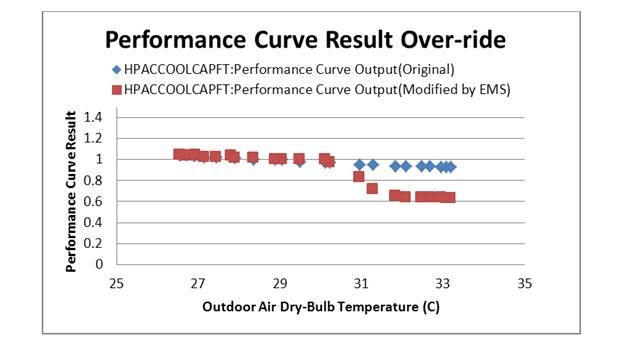
\includegraphics[width=0.9\textwidth, height=0.9\textheight, keepaspectratio=true]{media/image011.jpg}
\caption{Results of Performance Curve Override \protect \label{fig:results-of-performance-curve-override}}
\end{figure}


\section{Example 12. Variable Refrigerant Flow System Override}\label{example-12.-variable-refrigerant-flow-system-override}

\subsection{Problem Statement}\label{problem-statement-002}

The variable refrigerant flow heat pump air conditioner has several available thermostat control options. These operation control schemes may not provide the type of control desired. How can we use a simple EMS addition to an input file that can override the specified thermostat control logic and set an alternate mode of operation?

\subsection{EMS Design Discussion}\label{ems-design-discussion-002}

Depending on the type of thermostat control logic, the EnergyPlus program will review the loads in each zone, the number of zones in cooling or heating, the deviation from set point temperature, etc. to determine the mode of operation for the heat pump condenser. Alternate control logic may be developed to more accurately reflect the operation of a specific manufacturers product, or investigate other control techniques. This control logic may be added to an input file and used as the operating control logic of the heat pump.

This simple example shows how to use EMS actuators to SET the operating mode and cause a specific terminal unit to operate at a specified part-load ratio (PLR). When setting the terminal unit PLR, the terminal unit will turn on only if the condenser is allowed to operate according to the minimum and maximum outdoor temperature limits.

\subsection{EMS Input Objects}\label{ems-input-objects-002}

The main input objects that implement this example are the variable refrigerant flow actuators that control the VRF system and specific terminal unit. Note that the terminal unit PLR can be controlled without controlling the mode of the VRF condenser, however, the specific terminal unit will operate in whatever mode the existing operation control scheme chooses. This example program simply ``sets'' the operating mode and PLR, other more complex control algorithms can be developed by the user as needed.

\begin{lstlisting}

  Output:EnergyManagementSystem,
      Verbose,                 !- Actuator Availability Dictionary Reporting
      Verbose,                 !- Internal Variable Availability Dictionary Reporting
      Verbose;                 !- EMS Runtime Language Debug Output Level


    EnergyManagementSystem:ProgramCallingManager,
      VRF OnOff Management,     !- Name
      InsideHVACSystemIterationLoop,  !- EnergyPlus Model Calling Point
      VRFControl;               !- Program Name 1


    EnergyManagementSystem:Program,
      VRFControl,               !- Name
      SET VRF_Actuator_OnOff = VRF_Status_Heating, !- Program Line 2
      SET VRF_TerminalUnit1_PLR = 0.5;


    EnergyManagementSystem:Actuator,
      VRF_Actuator_OnOff,       !- Name
      VRF Heat Pump,            !- Actuated Component Unique Name
      Variable Refrigerant Flow Heat Pump,      !- Actuated Component Type
      Operating Mode;           !- Actuated Component Control Type


    EnergyManagementSystem:Actuator,
      VRF_TerminalUnit1_PLR,    !- Name
      TU1,                      !- Actuated Component Unique Name
      Variable Refrigerant Flow Terminal Unit,  !- Actuated Component Type
      Part Load Ratio;          !- Actuated Component Control Type


    EnergyManagementSystem:OutputVariable,
      Erl VRF Control Status,   !- Name
      VRF_Actuator_OnOff,       !- EMS Variable Name
      Averaged,                 !- Type of Data in Variable
      SystemTimeStep;           !- Update Frequency


    Output:Variable,*,Erl VRF Control Status, detailed;
    Output:Variable,*,VRF Heat Pump Operating Mode, detailed;
    Output:Variable,*,Cooling Coil Runtime Fraction, detailed;
    Output:Variable,*,Heating Coil Runtime Fraction, detailed;


    EnergyManagementSystem:ProgramCallingManager,
      Init VRF Control Mode Constants,  !- Name
      BeginNewEnvironment,           !- EnergyPlus Model Calling Point
      InitializeVRFControlModes;     !- Program Name 1


    EnergyManagementSystem:Program,
      InitializeVRFControlModes,     !- Name
      Set VRF_Status_Off = 0.0,      !- Program Line 1
      Set VRF_Status_Cooling = 1.0,  !- Program Line 2
      Set VRF_Status_Heating = 2.0;  !- Program Line 3


    EnergyManagementSystem:GlobalVariable,
      VRF_Status_Off,                !- Erl Variable 1 Name
      VRF_Status_Cooling,            !- Erl Variable 2 Name
      VRF_Status_Heating;            !- Erl Variable 3 Name
\end{lstlisting}


\section{Example 13. Surface Construction Actuator for Thermochromic Window}\label{example-13.-surface-construction-actuator-for-thermochromic-window}

\subsection{Problem Statement}\label{problem-statement-003}

There are a variety of novel new technologies for dynamic thermal envelopes that are the subject of research and development. Can we use EMS to investigate dynamic envelope technologies?

\subsection{EMS Design Discussion}\label{ems-design-discussion-003}

As an example, we will show how to use the EMS to replicate a thermochromic window.~ EnergyPlus already has a dedicated model for thermochromic windows (see the input object WindowMaterial:GlazingGroup:Thermochromic) that is demonstrated in the example file called ThermochromicWindow.idf.~ For this EMS example we will start with that file, remove the WindowMaterial:GlazingGroup:Thermochromic and emulate the thermochromic window using the EMS actuator called ``Surface'' with the control type ``Construction State.''

The first step is to create the individual Construction objects that will represent the individual states.~ The original thermochromic example file already includes a series of WindowMaterial:Glazing input objects that correspond to the properties of the thermochromic glazing at different temperatures.~ These glazing layers are then used in a series of Construction objects that represent the entire glazing system description at each temperature ``state.''~ Separate EnergyManagementSystem:ConstructionIndexVariable objects are then added for each Construction to setup Erl variables that point to each construction.

The control algorithm is very simple.~ The temperature of the glazing is used in a long IF-ELSEIF-ELSE-ENDIF block to select the appropriate construction to assign the surface.~ In this case the native thermochromic model has an important advantage in that the dedicated model can access the temperature of the middle pane in a triple glazed window whereas the EMS model can only access the temperature of the outside pane or the inside pane.~ Here we use the temperature of the outside face of the surface because it is closer to the temperature of the middle pane (which can be much higher when in direct sun).

\subsection{EMS Input Objects}\label{ems-input-objects-003}

The main input objects that implement this example of EMS-based thermochromic glazing system are listed below.~ The surface called ``Perimeter\_ZN\_1\_wall\_south\_Window\_1'' is the one being actuated by EMS and we can observe the outcomes of the override by reporting the output variable called Surface Construction Index.~ See the example file called EMSThermochromicWindow.idf.

\begin{lstlisting}

  Construction,
      TCwindow_25,                !- Name
      Clear3PPG,               !- Outside Layer
      AIR 3MM,                 !- Layer 2
      WO18RT25,              !- Layer 3
      AIR 8MM,                 !- Layer 4
      SB60Clear3PPG;           !- Layer 5


    EnergyManagementSystem:ConstructionIndexVariable,
      TCwindow_25,
      TCwindow_25;


    Construction,
      TCwindow_27,                !- Name
      Clear3PPG,               !- Outside Layer
      AIR 3MM,                 !- Layer 2
      WO18RT27,              !- Layer 3
      AIR 8MM,                 !- Layer 4
      SB60Clear3PPG;           !- Layer 5


    EnergyManagementSystem:ConstructionIndexVariable,
      TCwindow_27,
      TCwindow_27;
  <<SNIPPED states between 27C and 80C>>


    Construction,
      TCwindow_80,                !- Name
      Clear3PPG,               !- Outside Layer
      AIR 3MM,                 !- Layer 2
      WO18RT80,              !- Layer 3
      AIR 8MM,                 !- Layer 4
      SB60Clear3PPG;           !- Layer 5


    EnergyManagementSystem:ConstructionIndexVariable,
      TCwindow_80,
      TCwindow_80;


    Construction,
      TCwindow_85,                !- Name
      Clear3PPG,               !- Outside Layer
      AIR 3MM,                 !- Layer 2
      WO18RT85,              !- Layer 3
      AIR 8MM,                 !- Layer 4
      SB60Clear3PPG;           !- Layer 5


    EnergyManagementSystem:ConstructionIndexVariable,
      TCwindow_85,
      TCwindow_85;


    EnergyManagementSystem:Sensor,
      Win1_Tout,
      Perimeter_ZN_1_wall_south_Window_1,
      Surface Outside Face Temperature;


    EnergyManagementSystem:Actuator,
      Win1_Construct,
      Perimeter_ZN_1_wall_south_Window_1,
      Surface,
      Construction State;


    EnergyManagementSystem:ProgramCallingManager,
      My thermochromic window emulator,
      BeginTimestepBeforePredictor,
      ZN_1_wall_south_Window_1_Control;


    EnergyManagementSystem:Program,
      ZN_1_wall_south_Window_1_Control,
      IF Win1_Tout < = 26.0 ,
        Set Win1_Construct = TCwindow_25,
      ELSEIF Win1_Tout < = 28.0 ,
        SEt Win1_Construct = TCwindow_27,
      ELSEIF Win1_Tout < = 30.0 ,
        SET Win1_Construct = TCwindow_29,
      ELSEIF Win1_Tout < = 32.0 ,
        SET Win1_Construct = TCwindow_31,
      ELSEIF Win1_Tout < = 34.0 ,
        SET Win1_Construct = TCwindow_33,
      ELSEIF Win1_Tout < = 36.0 ,
        SET Win1_Construct = TCwindow_35,
      ELSEIF Win1_Tout < = 38.0 ,
        SET Win1_Construct = TCwindow_37,
      ELSEIF Win1_Tout < = 40.0 ,
        SET Win1_Construct = TCwindow_39,
      ELSEIF Win1_Tout < = 42.0 ,
        SET Win1_Construct = TCwindow_41,
      ELSEIF Win1_Tout < = 44.0 ,
        SET Win1_Construct = TCwindow_43,
      ELSEIF Win1_Tout < = 47.5 ,
        SET Win1_Construct = TCwindow_45,
      ELSEIF Win1_Tout < = 52.5 ,
        SET Win1_Construct = TCwindow_50,
      ELSEIF Win1_Tout < = 57.5 ,
        SET Win1_Construct = TCwindow_55,
      ELSEIF Win1_Tout < = 62.5 ,
        SET Win1_Construct = TCwindow_60,
      ELSEIF Win1_Tout < = 67.5 ,
        SET Win1_Construct = TCwindow_65,
      ELSEIF Win1_Tout < = 72.5 ,
        SET Win1_Construct = TCwindow_70,
      ELSEIF Win1_Tout < = 77.5 ,
        SET Win1_Construct = TCwindow_75,
      ELSEIF Win1_Tout < = 82.5 ,
        SET Win1_Construct = TCwindow_80,
      ELSE ,
        SET Win1_Construct = TCwindow_85,
      ENDIF;


  Output:Variable, Perimeter_ZN_1_wall_south_Window_1, Surface Construction Index, timestep;
\end{lstlisting}


\chapter{Debugging EMS Programs}\label{debugging-ems-programs}

This section discusses approaches to debugging Erl programs. As you develop your own programs, you will need to identify and correct coding problems. The task of debugging an Erl program is challenging. Compared to most programming, with integrated development environments and sophisticated debugging interfaces, the Erl programmer has only rudimentary tools available for debugging. If you have some type of developer license and EnergyPlus source code, you could debug Erl programs inside a full-featured debugging environment (such as IVF integrated into VS9). But this is only for extremely advanced users and developers implementing EMS related code inside EnergyPlus. Most users' EMS should have little need to deal with compilers and development environments, because enough information is produced by EnergyPlus when it runs their Erl programs. This section examines output related to EMS in an effort to help you debug your Erl programs.


\section{ERR File}\label{err-file}

A key output file to review is the ERR file (eplusout.err), the one with the ``.err'' file extension. This is the common error file for all of EnergyPlus, and many EMS-related errors will appear there. The file might contain critical problems that arose while the Erl programs were being read in and processed. Although the EDD file will likely be the focus of most debugging, remember the ERR file. Also, sometimes no EDD file is produced from a run. This occurs when problems are captured early during input processing and the program fatals out before an Erl program is run. Depending on the run manager you use to execute EnergyPlus, the EDD file may be from a previous run, so check the file creation times for ERR and EDD.

An especially important error revealed in the ERR file is truncation from too long input. Each program line in Erl is limited to 100 characters. (It becomes useful to keep variable names shorter in Erl because the line length limit can be onerous.)~ If there are more than 100 characters, the program truncates the line to the first 100. This will often throw a severe error that halts because the truncated line is not a valid statement. But an unlucky truncation may form a viable line of code and the program will run. Truncation of any Erl program line is surely a bad thing, so it is important to check the ERR file.


\section{EDD File}\label{edd-file}

If the Erl programs are processed and start running, the EDD becomes a primary source of information for debugging. The EDD file is the output file associated only with the EMS. When a line of Erl code is executed, and full trace is selected, the program will output records that are useful for debugging.

It is very important to be careful with the EDD file. There are options to control how verbose the EDD file becomes with modes such as only the errors or a full trace. The full trace option should be used with care because a full line-by-line trace of EMS program execution for an annual run can easily create an enormous file that is too large for most computer systems.


\section{Line Trace}\label{line-trace}

You can use the EDD file to examine the execution of every line of code. If you request a verbose level of debugging output in the Output:EnergyManagementSystem input object, the EDD file will contain a series of text records that trace the execution of each line of Erl code. Traces contain the name of the program, the program line number, the text of the line, the result returned by executing the line (if any), and a timestamp that indicates when it was executed during the environment period. Note that the EDD file is only produced if you have EMS/Erl programs in your input file.

An example of a single trace follows. This is one record, or single line of text from one of the traces in an EDD file.

\begin{lstlisting}
VAV1MIXEDAIRMANAGERS,Line 1,SET VAV_1_COOLC_SETPOINT = SEASONAL_RESET_SAT_SCHED - ( T_VAV1FANOUT - T_VAV1FANIN),13.0000000000000, During Warmup, Occurrence info = CHICAGO IL USA TMY2-94846 WMO\# = 725300, 01/01 18:30 - 18:45
\end{lstlisting}

Each block of text is separated by comma, so the trace information could be read into a spreadsheet and formatted to columns using comma separation.

``VAV1MIXEDAIRMANAGERS'' is the name of a user-defined Erl Program.

``Line 1'' indicates that this trace is from the first line of the Erl program called VAV1MIXEDAIRMANAGERS.

The next block of text, ``SET VAV\_1\_COOLC\_SETPOINT = SEASONAL\_RESET\_SAT\_SCHED - ( T\_VAV1FANOUT - T\_VAV1FANIN)'' is the Erl program statement contained at Line 1 in the Erl program called VAV1MIXEDAIRMANAGERS.

The value ``13.0000000000000'' is the result of this particular SET statement. The value of 13.0 has been assigned to the variable called VAV\_1\_COOLC\_SETPOINT.

The next block of text ``During Warmup'' indicates that the line was executed while the simulation was in a warm up phase. (Warmup happens during the beginning of each environment period to precondition the model's transients with the conditions of the first day.)

The next block of text ``Occurrence info = CHICAGO IL USA TMY2-94846 WMO\# = 725300'' indicates the environment period being simulated. This is a weather-file-based RunPeriod for Chicago using TMY2 data source associated with weather station number 725300.

The last block of text ``01/01 18:30 - 18:45'' is the date and time of day for the simulation timestep when the Erl program line was executed.


\section{Debugging Strategies}\label{debugging-strategies}

This section attempts to provide some debugging tips.

There is no debugging environment, so the main way to obtain information is to use verbose mode and trace each line.

Say, for example, we are trying to debug the following line:

\begin{lstlisting}
 ELSEIF (Hour > = 5) && (Hour < 19)  && (DayOfWeek > = 2) && (DayOfWeek < = 6) ,
\end{lstlisting}

The line trace, shown next, shows only the result of the logical condition, i.e., 0.0 (highlighted) if overall it is false or 1.0 if overall it is true.

\begin{lstlisting}
MYCOMPUTEDHEATINGSETPOINTPROG,Line 10,ELSEIF (HOUR > = 5) && (HOUR < 19)  && (DAYOFWEEK > = 2) && (DAYOFWEEK < = 6),0.0, Occurrence info = CHICAGO IL USA TMY2-94846 WMO\# = 725300, 09/23 10:20 - 10:30
\end{lstlisting}

To debug what is going on with the individual terms in the logical expression, we can add some otherwise useless statements so line traces contain an echo of the current values of the HOUR and DAYOFWEEK built-in variables. So if we add the following lines before the start of the IF block,

\begin{lstlisting}
    Set locHour = Hour, ! echo out for debug
    Set locDay = DayOfWeek, ! echo out for debug
\end{lstlisting}

We will see the values that Hour and DayOfWeek contain in the debug output. The local variables Erl variables locHour and locDay do not need to be used for anything, but by adding these Erl statements we can glean debugging insights.

The line of Erl code is switched to all uppercase on input, so the line trace differs from the input file in that all characters are capitalized. If the input file was developed using a CamelCase convention, it may be much more difficult to read in the line trace output. Thus, the underscore character ``\_'' may be a more useful convention for inputting Erl code because it will be more readable in the debugging traces.


\end{document}
